% =========================================================================
% SciPost LaTeX template
% Version 2024-07
%
% Submissions to SciPost Journals should make use of this template.
%
% INSTRUCTIONS: simply look for the `TODO:' tokens and adapt your file.
% ========================================================================

\documentclass{SciPost_better_arXiv}

% Prevent all line breaks in inline equations.
\binoppenalty=10000
\relpenalty=10000
\emergencystretch=3em % Give LaTeX a bit more slack with breaking lines
\hypersetup{
    colorlinks,
    linkcolor={red!50!black},
    citecolor={blue!50!black},
    urlcolor={blue!80!black}
}

\usepackage[bitstream-charter]{mathdesign}
\urlstyle{same}

% Fix \cal and \mathcal characters look (so it's not the same as \mathscr)
\DeclareSymbolFont{usualmathcal}{OMS}{cmsy}{m}{n}
\DeclareSymbolFontAlphabet{\mathcal}{usualmathcal}

\usepackage{hyperref}
\usepackage{cleveref}
\usepackage{booktabs}
\usepackage{xcolor}
\usepackage{multirow}
\usepackage{pdflscape}
\usepackage{placeins}
\usepackage{graphicx}

\newcommand{\HRule}{\rule{\linewidth}{0.5mm}}
\renewcommand*{\thefootnote}{\fnsymbol{footnote}}
\newcommand{\MH}{M_\mathrm{H}}
\newcommand{\VBF}{\mathrm{VBF}}
\newcommand{\DIS}{\mathrm{DIS}}
\newcommand{\QCD}{\mathrm{QCD}}
\newcommand{\ELWK}{\mathrm{EW}}
\newcommand{\NNLO}{\mathrm{NNLO}}
\newcommand{\NNNLO}{\mathrm{N3LO}}
\newcommand{\alphas}{\alpha_{\mathrm{s}}}
\newcommand{\GeV}{~\mathrm{GeV}}
\newcommand{\OS}{\mathrm{OS}}

\newcommand{\gencomment}[3]{\textcolor{#2}{[#1]$_\text{#3}$}}
\newcommand{\ak}[1]{\gencomment{#1}{blue}{AK}}
\newcommand{\comment}[1]{\gencomment{#1}{orange}{all}}


\fancypagestyle{SPstyle}{
\fancyhf{}
\lhead{\colorbox{scipostblue}{\bf \color{white} ~SciPost Physics Community Reports }}
\rhead{{\bf \color{scipostdeepblue} ~Submission }}
\renewcommand{\headrulewidth}{1pt}
\fancyfoot[C]{\textbf{\thepage}}
}

\begin{document}

\pagestyle{SPstyle}
\begin{flushright}
LHCHWG-2026-005, FR-PHENO-2026-012, MPP-2026-150, OUTP-26-05P, TIF-UNIMI-2025-29, TTK-26-35, TTP26-035
\end{flushright}
\begin{center}{\Large \textbf{\color{scipostdeepblue}{
%%%%%%%%%% TODO: Write your article's title here
Predictions for Inclusive Production Cross Sections of the Higgs~Boson at the LHC and HL-LHC\\
%%%%%%%%%% END TODO: TITLE
}}}\end{center}

\begin{center}\textbf{
%%%%%%%%%% TODO: AUTHORS
% Write the author list here. 
% Use (full) first name (+ middle name initials) + surname format.
% Separate subsequent authors by a comma, omit comma and use "and" for the last author.
% Mark the corresponding author(s) with a superscript symbol in this order
    % \star, \dagger, \ddagger, \circ, \S, \P, \parallel, ...
    {\it Editors$^\star$:} Robin~Hayes$^{1\dagger}$, Alexander~Karlberg$^{2\ddagger}$, Bernhard~Mistlberger$^{3\circ}$,
    Dermot~Moran$^{4\S}$\\[0.3cm]
%
    {\it Contributors:}
    Hannah~Arnold$^{5}$,
    Gaetano~Barone$^{6}$,
    Christian~Biello$^{7}$,
    Valeria~Botta\textcolor{red}{$^{?}$},
    Christian~Br{\o}nnum-Hansen$^{8}$,
    Alessandro~Calandri$^{9}$,
    Alessandra~Cappati\textcolor{red}{$^{?}$},
    Andrea~Cardini$^{10}$,
    Suman~Chatterjee$^{11}$,
    Jiayi~Chen$^{12}$,
    Valerio~Dao$^{5}$,
    Silvia~Ferrario~Ravasio$^{13}$,
    Giancarlo~Ferrera$^{14}$,
    Alessandro~Gavardi$^{13}$,
    Yanping~Huang$^{15}$,
    Alexander~Huss$^{16}$,
    Stephen~Jones$^{17}$,
    Judith~Katzy$^{11}$,
    Matthew~Lim$^{18,19}$,
    Josh~McFayden$^{18}$,
    Alexander~M\"uck$^{20}$,
    Mathieu~Pellen$^{21}$,
    Christian~T.~Preuss$^{20}$,
    Michael~Spira$^{22}$,
    Lourdes~Urda~G\'omez$^{23}$,
    Marco~Vitti$^{8}$,
    Marius~Wiesemann$^{24}$,
    Malgorzata~Worek$^{20}$,
    Silvia~Zanoli$^{25}$,
    Marco~Zaro$^{26}$ and
    Licheng~Zhang$^{27}$
%%%%%%%%%% END TODO: AUTHORS
}\end{center}

\begin{center}
%%%%%%%%%% TODO: AFFILIATIONS
% Write all affiliations here.
% Format: institute, city, country
  {\bf 1} Nikhef, Science Park 105, 1098 XG Amsterdam, The Netherlands \\
  {\bf 2} Max Planck Institute for Physics, Boltzmannstr. 8, 85748 Garching, Germany \\
  {\bf 3} SLAC National Accelerator Laboratory, Stanford University, Stanford, CA 94039, USA  \\
  {\bf 4} CIEMAT, Av. Complutense, 40, 28040 Madrid, Spain \\
  {\bf 5} Departments of Physics and Astronomy, Stony Brook University, Stony Brook, NY, United States of America\\
  {\bf 6} Department of Physics, Brown University, 182 Hope Street, Providence, RI 02912, USA\\
  {\bf 7} Institute for Theoretical Physics, ETH Zurich, 8093 Z\"urich, Switzerland\\
  {\bf 8} Institute for Theoretical Particle Physics, Karlsruhe Institute of Technology (KIT), Wolfgang-Gaede-Stra\ss{}e 1, 76131 Karlsruhe, Germany\\
  {\bf 9} Universit\`{a} degli Studi di Firenze \& INFN, Sezione di Firenze, Via Sansone 1, 50019 Sesto Fiorentino, Italy\\
  {\bf 10} Universidad de Oviedo, Instituto Universitario de Ciencias y Tecnolog\'{\i}as Espaciales de Asturias (ICTEA), Oviedo, Spain\\
  {\bf 11} Deutsches Elektronen-Synchrotron DESY, Notkestrasse 85, 22607 Hamburg, Germany\\
  {\bf 12} Department of Physics, 8888 University Dr W, Burnaby, BC V5A1S6, Canada\\
  {\bf 13} Universit\`{a} degli Studi di Torino \& INFN, Sezione di Torino, Via Giuria 1, 10125 Torino, Italy\\
  {\bf 14} Dipartimento di Fisica, Universit\`{a} di Milano \& INFN, Sezione di Milano, I-20133 Milan, Italy\\
  {\bf 15} Institute of High Energy Physics, Chinese Academy of Sciences, Beijing, China\\
  {\bf 16} Theoretical Physics Department, CERN, 1211 Geneva 23, Switzerland\\
  {\bf 17} Institute for Particle Physics Phenomenology, Durham University, South Road, Durham DH1 3LE, UK\\
  {\bf 18} Department of Physics and Astronomy, School of Mathematical and Physical Sciences, University of Sussex, Brighton, BN1 9RH, UK\\
  {\bf 19} Universit\`{a} degli Studi di Milano-Bicocca \& INFN Sezione di Milano-Bicocca, Piazza della Scienza 3, Milano 20126, Italy\\
  {\bf 20} Institut f\"ur Theoretische Teilchenphysik und Kosmologie, RWTH Aachen University, 52056 Aachen, Germany\\
  {\bf 21} Physikalisches Institut, Albert-Ludwigs-Universit\"at Freiburg, D-79104 Freiburg, Germany\\
  {\bf 22} PSI Center for Neutron and Muon Sciences, CH-5232 Villigen PSI, Switzerland\\
  {\bf 23} The Institute of Modern Physics (IMP) of the Chinese Academy of Sciences, Fudan University, Shanghai (China)\\
  {\bf 24} Department of Physics, TU Dortmund University, 44227 Dortmund, Germany\\
  {\bf 25} Rudolf Peierls Centre for Theoretical Physics, Clarendon Laboratory, Parks Road, Oxford OX1 3PU, UK\\
  {\bf 26} TIFLab, Universit\`{a} degli Studi di Milano \& INFN, Sezione di Milano, Via Celoria 16, 20133 Milano, Italy\\
  {\bf 27} Department of Physics, University of Maryland, College Park (UMD), 20742 College Park, USA\\
  {\bf \textcolor{red}{?}} \textcolor{red}{Affiliation missing}
 %%%%%%%%%% END TODO: AFFILIATIONS
%%%%%%%%%% TODO: EMAIL
% Provide email address of corresponding author(s)
\\[\baselineskip]
$\star$~\href{mailto:lhc-higgs-xsbr-convener@cern.ch}{\small lhc-higgs-xsbr-convener@cern.ch}\,,\quad
$\dagger$~\href{mailto:robin.hayes@cern.ch}{\small robin.hayes@cern.ch}\,,\quad
$\ddagger$~\href{mailto:alexander.karlberg@cern.ch}{\small alexander.karlberg@cern.ch}\,,\quad
$\circ$~\href{mailto:bernhard@slac.stanford.edu}{\small bernhard@slac.stanford.edu}\,,\quad
$\S$~\href{mailto:dermot.anthony.moran@cern.ch}{\small dermot.anthony.moran@cern.ch}
%%%%%%%%%% END TODO: EMAIL
\end{center}

\section*{\color{scipostdeepblue}{Abstract}}
\textbf{\boldmath{%
We present updated recommendations of the LHC Higgs Working Group (LHCHWG) for
the inclusive production cross sections of a Standard Model Higgs boson in
proton--proton collisions at centre-of-mass energies between $7$ and $14$~TeV,
including the Run-3 energy of $13.6$~TeV, and for Higgs-boson masses between
$120$ and $130$~GeV. Gluon fusion, vector-boson fusion, associated production
with a vector boson, associated production with a top-quark pair or a single top quark, and associated production with
bottom quarks are covered. The central values remain consistent with those of
Yellow Report~4 (YR4)~\cite{LHCHiggsCrossSectionWorkingGroup:2016ypw} within
the uncertainties quoted there, while the theoretical uncertainties are reduced
for most production modes. For gluon fusion we examine in detail the impact of
approximate N$^3$LO parton distribution functions (PDFs) and of QED corrections
to the DGLAP evolution; the tension between NNLO and approximate N$^3$LO sets
leads us to double the uncertainty assigned to the mismatch between the
N$^3$LO matrix element and NNLO PDFs. PDFs are now the leading source of
uncertainty for the most precisely predicted modes, while residual
perturbative uncertainties dominate for the remainder. These results supersede the
inclusive cross sections of YR4 and the ad interim recommendations of
Ref.~\cite{Karlberg:2024zxx}, and form part of Report~5 of the LHCHWG.
}}
\vspace{\baselineskip}

%%%%%%%%%% BLOCK: Copyright information
% This block will be filled during the proof stage, and finilized just before publication.
% It exists here only as a placeholder, and should not be modified by authors.
\noindent\textcolor{white!90!black}{%
\fbox{\parbox{0.975\linewidth}{%
\textcolor{white!40!black}{\begin{tabular}{lr}%
  \begin{minipage}{0.6\textwidth}%
    {\small Copyright attribution to authors. \newline
    This work is a submission to SciPost Phys. Comm. Rep. \newline
    License information to appear upon publication. \newline
    Publication information to appear upon publication.}
  \end{minipage} & \begin{minipage}{0.4\textwidth}
    {\small Received Date \newline Accepted Date \newline Published Date}%
  \end{minipage}
\end{tabular}}
}}
}
%%%%%%%%%% BLOCK: Copyright information


%%%%%%%%%% TODO: LINENO
% For convenience during refereeing we turn on line numbers:
\linenumbers
% You should run LaTeX twice in order for the line numbers to appear.
%%%%%%%%%% END TODO: LINENO
\clearpage
%%%%%%%%%% TODO: TOC 
% Guideline: if your paper is longer that 6 pages, include a TOC
% To remove the TOC, simply cut the following block
\vspace{10pt}
\noindent\rule{\textwidth}{1pt}
\tableofcontents
\noindent\rule{\textwidth}{1pt}
\vspace{10pt}
%%%%%%%%%% END TODO: TOC


%%%%%%%%% TODO: CONTENTS 
% Write your article contents here, starting from first \section.
% An example structure is given below.

%%%%%%%%%%%%%%%%%%%%%%%%%%%%%%%%%%%%%%%%%  Intro
%\clearpage
\section{Introduction}
\label{sec:intro}
\renewcommand*{\thefootnote}{\arabic{footnote}}
\setcounter{footnote}{0} \setcounter{page}{1}
The discovery of a scalar particle compatible with the Standard Model
(SM) Higgs boson by the ATLAS and CMS collaborations in
2012~\cite{ATLAS:2012yve,CMS:2012qbp} completed the particle content
of the SM and inaugurated a systematic and ever more precise
experimental study of the Higgs sector. In the years since, the LHC
experiments have measured the mass, spin, parity, and couplings of the
Higgs boson in ever finer detail. Combined analyses of the full LHC
Run-2 dataset by ATLAS and CMS~\cite{ATLAS:2022vkf,CMS:2022dwd},
together with more recent updates based on the complete Run-2
sample~\cite{ATLAS:2026comb,CMS:2026nce}, have established the
couplings of the Higgs boson to third-generation fermions and to the
electroweak gauge bosons at the level of a few to ten percent,
found evidence for its decay to muons, and set increasingly stringent limits on
its couplings to light quarks, its total width, possible CP-violating
admixtures, and on Higgs boson pair production, which probes the
trilinear self-coupling directly.  The LHC is now operating in Run 3
at a centre-of-mass energy of $\sqrt{s}=13.6$~TeV, and the
High-Luminosity LHC (HL-LHC) is expected to ultimately deliver up to
$3$--$4\,\mathrm{ab}^{-1}$ per experiment, which will reduce
the statistical uncertainties on many Higgs-boson observables to the
percent level or below~\cite{Cepeda:2019klc}.

This remarkable experimental progress, and the even higher precision
anticipated at the HL-LHC, places correspondingly stringent demands on
the accuracy of the theoretical predictions used to interpret the
data. For several production and decay channels, the precision of
current measurements is already comparable to, or in some cases better
than, the theoretical uncertainties quoted in the most recent
comprehensive reference for Higgs production cross sections, the CERN
Yellow Report~4 (YR4)~\cite{LHCHiggsCrossSectionWorkingGroup:2016ypw},
compiled by the LHC Higgs Cross Section Working Group (LHCHWG) in
2016. Moreover, YR4 does not provide predictions at
$\sqrt{s}=13.6$~TeV, the current LHC operating energy; an interim
interpolation was subsequently provided by the working
group~\cite{Karlberg:2024zxx} as a stop-gap measure pending a full
update. Both of these facts make clear that a systematic update of the
SM predictions for all Higgs-boson production modes, incorporating the
theoretical progress of the past decade, is both timely and necessary
if the LHC and HL-LHC precision programmes are to be fully exploited.

Since the publication of YR4, the theoretical description of every
production mode considered here has advanced. For gluon fusion, the
dominant mode, the inclusive cross section in the heavy-top limit is
now known exactly at N$^3$LO in
QCD~\cite{Anastasiou:2015vya,Anastasiou:2016cez,Mistlberger:2018etf},
rather than through a threshold expansion. It has been supplemented by
exact finite-quark-mass corrections at NNLO, both for the top-only
contribution~\cite{Czakon:2020vql,Czakon:2021yub,Czakon:2024ywb} and
for the top--bottom interference~\cite{Czakon:2023kqm,Czakon:2024ywb},
by mixed QCD--electroweak corrections to the gluon-induced channel
retaining the full dependence on the electroweak boson
masses~\cite{Bonetti:2016brm,Bonetti:2017ovy,Bonetti:2018ukf,Becchetti:2020wof},
and by an approximate N$^4$LO result obtained in the soft-virtual
approximation~\cite{Das:2020adl}. Vector-boson fusion is available at
N$^3$LO in the structure-function approximation~\cite{Dreyer:2016oyx},
and the non-factorisable corrections neglected in that approximation
have since been computed~\cite{Liu:2019tuy,Dreyer:2020urf,Asteriadis:2023nyl}.
Associated production with a $W$ or $Z$ boson has reached N$^3$LO QCD
accuracy for the Drell--Yan-like
contribution~\cite{Baglio:2022wzu}, and the NLO QCD corrections to the
loop-induced $gg\to ZH$ channel have been completed with full
top-quark mass
dependence~\cite{Altenkamp:2012sx,Hasselhuhn:2016rqt,Davies:2020drs,Chen:2020gae,Wang:2021rxu,Alasfar:2021ppe,Chen:2022rua,Degrassi:2022mro,Davies:2025out},
with first NNLO results in the large-$m_t$ limit appearing
recently~\cite{Davies:2025otz}. For $t\bar{t}H$, the NNLO QCD
corrections~\cite{Catani:2022mfv,Devoto:2024nhl} have been matched to
NNLL soft-gluon resummation and combined with the complete NLO
electroweak corrections~\cite{Balsach:2025jcw}. Single-top associated
production remains known at NLO QCD~\cite{Demartin:2015uha,Demartin:2016axk};
NLO electroweak corrections are also available, but only for the three
production channels taken together, since the separation into channels
is no longer well defined once they are
included~\cite{Pagani:2020mov}. Production in association with bottom
quarks has reached N$^3$LO accuracy in the five-flavour
scheme~\cite{Duhr:2019kwi} and has been matched to the four-flavour
scheme at that order using the FONLL method~\cite{Duhr:2020kzd}; the
recommendation presented below is instead based on the
NLO+NNLL\textsubscript{part} matching of
Refs.~\cite{Bonvini:2015pxa,Bonvini:2016fgf}, which allows an explicit
resummation-scale uncertainty to be assigned.

The parton distribution functions (PDFs) entering all of these
predictions have been refined in parallel. The PDF4LHC21
combination~\cite{PDF4LHCWorkingGroup:2022cjn} is the recommended NNLO
baseline and is used throughout this report. Beyond NNLO, approximate
N$^3$LO sets have been produced by the MSHT and NNPDF
collaborations~\cite{McGowan:2022nag,NNPDF:2024nan}, benchmarked
against one another~\cite{Cooper-Sarkar:2024crx} and subsequently
combined~\cite{Cridge:2024icl}. Separately, the effect of QED
corrections to the DGLAP evolution has been quantified for Higgs
production for the first time~\cite{Manohar:2016nzj,Cooper-Sarkar:2025sqw}.
Both developments bear on gluon fusion more than on any other mode,
since the hard-scattering cross section is known one order beyond the
PDFs and since sub-percent changes in the gluon luminosity are no
longer negligible at the precision now reached. They are introduced in
Section~\ref{sec:setup} and their consequences for the recommendation
are worked out in Section~\ref{sec:ggF}.

The LHCHWG is currently preparing a set of updates which will
collectively replace YR4, published as a series of reports in SciPost
Physics Community Reports and referred to in the following as Report~5
(R5). Where numerical predictions are compared, R5 denotes the recommendations
of the present report and YR4 those of its predecessor. Several of these have already appeared, among them dedicated
studies of vector-boson fusion~\cite{Barone:2025jey}, of
$t\bar{t}H$~\cite{Balsach:2025jcw}, of the $gg\to ZH$
channel~\cite{CampilloAveleira:2025rbh}, and of the modelling of
$b\bar{b}H$ production~\cite{10.21468/SciPostPhysCommRep.18}. The
present report is the contribution to R5 concerned with inclusive
production cross sections. It collects the developments listed above
into an updated set of LHCHWG recommendations at
$\sqrt{s}=7,\,8,\,13,\,13.6$, and $14$~TeV and for Higgs-boson masses
between $120$ and $130$~GeV, covering gluon fusion (ggF), vector-boson
fusion (VBF), associated production with a $W$ or $Z$ boson (VH),
associated production with a top-quark pair ($t\bar{t}H$) or a single
top quark ($tH$), and associated production with bottom quarks
($b\bar{b}H$). For $t\bar{t}H$ and $tH$, predictions are provided at
$13$, $13.6$ and $14$~TeV only. For each production mode we document
the ingredients entering the recommendation, define the procedure by
which they are combined, and state the residual theoretical and
parametric uncertainties. We further place the resulting precision in
the context of the most precise current LHC measurements and of
projected HL-LHC
sensitivities~\cite{Cepeda:2019klc,ATLAS:2022hsp}, in order to assess
to what extent the present theoretical uncertainties will remain
sufficient, or become a limiting factor, over the coming decade of LHC
running. Within this scope the report supersedes
YR4~\cite{LHCHiggsCrossSectionWorkingGroup:2016ypw} and the ad interim
recommendations of Ref.~\cite{Karlberg:2024zxx}; branching ratios,
differential distributions and off-shell effects are not addressed
here.

The chapters that follow differ considerably in length, for two
reasons. For most production modes, the calculations entering the
recommendation and the reasoning behind the choices made in combining
them are discussed at length elsewhere in R5 and in the literature it
builds on. Those chapters therefore concentrate on the ingredients
that define the present prediction, on the combination formula and on
the uncertainty prescription, and point the reader onwards for the
supporting material. Gluon fusion is the exception. No such account
exists elsewhere, and the number of separate decisions that had to be
taken is in any case larger. The renormalisation scheme of the
top-quark mass, the finite quark-mass corrections now available at
NNLO, the mismatch between an N$^3$LO matrix element and NNLO PDFs,
and the inclusion of QED evolution each shift either the central value
or the uncertainty at the percent level, and they do not all act in
the same direction. Section~\ref{sec:ggF} consequently treats each
ingredient and its uncertainty in turn, in the manner of YR4, and is
correspondingly longer than the others. This unevenness reflects where
the work was needed rather than the relative importance of the
production modes.

The remainder of this report is organised as
follows. Section~\ref{sec:setup} defines the common input parameters
and conventions used throughout. Sections~\ref{sec:ggF}--\ref{sec:bbH}
present the state of the art and the resulting recommendations for
ggF, VBF, VH, $t\bar t H$/$tH$, and $b\bar b H$ production,
respectively. Section~\ref{sec:Outlook} discusses the resulting
uncertainties in comparison with YR4 and with current and projected
experimental precision, and Section~\ref{sec:conclusions}
concludes. Numerical tables for all production modes, collision
energies and Higgs-boson masses considered are collected in
Appendix~\ref{app:tables}; for gluon fusion these also contain the
information required to convert the recommendation to approximate
N$^3$LO PDFs. The numbers are additionally available at
\url{https://gitlab.cern.ch/LHCHIGGSXS/LHCHXSWG1/crosssections}.


%%%%%%%%%%%%%%%%%%%%%%%%%%%%%%%%%%%%%%%%% ggF
\section{Common setup}
\label{sec:setup}
\input{Chapters/setup.tex}

%%%%%%%%%%%%%%%%%%%%%%%%%%%%%%%%%%%%%%%%% ggF
\section{ggF}
\label{sec:ggF}
\input{Chapters/ggF.tex}

%%%%%%%%%%%%%%%%%%%%%%%%%%%%%%%%%%%%%%%%% VBF
\section{VBF}
\label{sec:VBF}
\input{Chapters/VBF.tex}

%%%%%%%%%%%%%%%%%%%%%%%%%%%%%%%%%%%%%%%%% VH
\section{VH}
\label{sec:VH}
\subsection{Summary of Theory Developments} 
In this section, we shortly collect results available for the theoretical description of the associated production of a Higgs boson and a weak vector boson (VH) at the LHC, and we outline recent developments in theory predictions. We recall that the dominant partonic contribution to the process comes from the $q\bar{q}$-initiated, Drell-Yan-like channel, while a subleading contribution due to a loop-induced $gg$-initiated channel arises at NNLO QCD for the $ZH$ final state.

Concerning fixed-order predictions, the QCD corrections for the $q \bar{q}$-initiated process have been known at NNLO~\cite{HAN1991167, Brein:2003wg}. For the Drell-Yan-like contribution, N$^3$LO QCD corrections have become available~\cite{Baglio:2022wzu}. Electroweak (EW) NLO corrections have been computed in Refs.~\cite{Ciccolini:2003jy, Denner:2011id} and are available in the \texttt{HAWK} code~\cite{Denner:2011id,Denner:2014cla}, including the leptonic decays of the weak bosons. Differential predictions are available in Refs.~\cite{Ferrera:2011bk, Ferrera:2013yga,Ferrera:2014lca,Campbell:2016jau,Gauld:2021ule}, including NNLO QCD and NLO EW effects.
In recent years, considerable interest has been devoted to the QCD corrections to the subdominant process $gg \to ZH$~\cite{Dicus:1988yh,Kniehl:1990iva}, with the aim of reducing the non-negligible impact of the associated scale uncertainties. The NLO QCD corrections have been obtained using multiple approaches~\cite{Altenkamp:2012sx,Hasselhuhn:2016rqt,Davies:2020drs,Chen:2020gae,Wang:2021rxu,Alasfar:2021ppe,Chen:2022rua,Degrassi:2022mro,Davies:2025out}. The Refs.~\cite{Chen:2022rua,Degrassi:2022mro} discuss an additional source of theoretical uncertainty due to the choice of renormalization scheme for the top-quark mass ($m_t$). More recently, QCD corrections at NNLO have been computed~\cite{Davies:2025otz} in the large-$m_t$ limit. 

Given the relevance of VH production as an experimental probe of the Higgs coupling to bottom quarks, several works have discussed the effects of supplementing VH predictions with the Higgs decay to a $b \bar{b}$ pair~\cite{Caola:2017xuq,Gauld:2019yng,Behring:2020uzq}.

The resummation of threshold logarithms for the Drell-Yan (DY) component of VH production has been carried out at N$^3$LL accuracy~\cite{Kumar:2014uwa, Das:2022zie}. Soft-gluon resummation in the $gg$-initiated channel has been studied in Refs.~\cite{Harlander:2014wda,Das:2025wbj,Das:2025qym}. The matching of fixed-order corrections to the parton shower (PS) has been obtained for VH production at NLO QCD~\cite{Luisoni:2013cuh,Granata:2017iod} and at NLO EW~\cite{Granata:2017iod} accuracy. Considering NNLO QCD corrections, merged predictions including one jet for $gg \to ZH$ have been presented~\cite{Hespel:2015zea, Goncalves:2015mfa}, while NNLO+PS predictions for the full VH process have been achieved in Refs.~\cite{Astill:2016hpa,Astill:2018ivh, Alioli:2019qzz}. Matched predictions including the $H\to b \bar{b}$ decay at full NNLO+PS accuracy have been obtained in Ref.~\cite{Zanoli:2021iyp}.

\subsection{Inclusive Cross Section Predictions}
\label{sec:vh_inclxs_breakdown}

The results compiled in Tables~\ref{tab:w+h_xs_7tev}-\ref{tab:zh_xs_14tev} are obtained from the following combination of the different contributions to the cross section
\begin{align}
    \sigma^{VH} &= \sigma_\mathrm{DY}^{VH}(1+ \delta_\mathrm{EW})+ \sigma_\text{top} + \delta_{\tiny VZ}~\sigma^\mathrm{NLO}_{ggZH},
    \label{eq:sigma_vh_breakdown}
\end{align}
where $\sigma_\mathrm{DY}^{VH}$ is the Drell-Yan-like contribution at NNLO QCD, $\delta_\mathrm{EW}$ is a multiplicative factor that accounts for the relative EW corrections at NLO, $\delta_{\tiny VZ}$ equals 1 when $V=Z$ and 0 otherwise, and $\sigma^\mathrm{NLO}_{ggZH}$ is the NLO QCD cross section for the $gg$-initiated channel. The term $\sigma_\text{top}$ is defined as
\begin{align}
     \sigma_\text{top} &= \sigma_\mathrm{I}^{VH} + \delta_{VZ}~\sigma_\mathrm{II}^{ZH},
\end{align}
where $\sigma_\mathrm{I}^{VH}$ and $\sigma_\mathrm{II}^{ZH}$ are contributions mediated by top-quark loops in the $q\bar{q}$-initiated channel.
The terms $\sigma^\mathrm{NLO}_{ggZH}$ and $\sigma_\mathrm{II}^{ZH}$  are present only in the $ZH$ final state. In the Tables~\ref{tab:w+h_xs_7tev}-\ref{tab:zh_xs_14tev} we provide results for on-shell bosons.

The results for all the contributions in Eq.~\eqref{eq:sigma_vh_breakdown} except $\sigma^\mathrm{NLO}_{ggZH}$ were always obtained using \texttt{vh@nnlo}~\cite{Harlander:2018yio}. The results for $\sigma^\mathrm{NLO}_{ggZH}$ at centre-of-mass (CM) energies $\sqrt{s}=\{13, 13.6, 14\}$~TeV are taken from Ref.~\cite{CampilloAveleira:2025rbh}, which includes NLO QCD corrections with top-quark mass effects at $\mathcal{O}(\%)$ accuracy. This reference provides a comparison of the virtual corrections reported in Refs.~\cite{Chen:2022rua,Degrassi:2022mro} and supplements the latter with the new results for the real corrections using \texttt{GoSam}~\cite{Braun:2025afl}. Results for values of the Higgs mass not present in Ref.~\cite{CampilloAveleira:2025rbh} have been obtained with a linear interpolation, which is accurate at $\mathcal{O}(10^{-4})$, given the mild dependence of the cross section on this parameter. For $\sqrt{s}=\{7, 8\}$~TeV, also the values of $\sigma^\mathrm{NLO}_{ggZH}$ are computed using \texttt{vh@nnlo}. 

The uncertainties due to the factorization and renormalization scale variation are denoted as $\Delta_\text{scale}$ and computed from a 7-point scale variation in the interval
\begin{align}
    M_{VH}/3 \leq \mu_F ,\mu_R \leq 3 M_{VH},
\end{align}
with $M_{VH}$ the invariant mass of the $VH$ system. Only in the case in which $\sigma^\mathrm{NLO}_{ggZH}$ is taken from Ref.~\cite{CampilloAveleira:2025rbh}, the scale uncertainties for the latter are obtained from a 7-point scale variation in the interval
\begin{align}
    M_{ZH}/4 \leq \mu_F ,\mu_R \leq M_{ZH}
\end{align}
and effects due to the different choice of scales are neglected. The PDF and $\alpha_s$ uncertainties (denoted as $\Delta_\text{PDF}$ ad $\Delta_{\alpha_s}$, respectively) are calculated following the recommendations in \url{https://twiki.cern.ch/twiki/bin/view/LHCPhysics/LHCHWG136TeVxsec}.





%%%%%%%%%%%%%%%%%%%%%%%%%%%%%%%%%%%%%%%%% ttH
\section{\texorpdfstring{$\boldsymbol{t\bar{t}H}$}{ttH} and \texorpdfstring{$\boldsymbol{tH}$}{tH}}
\label{sec:ttH}
\input{Chapters/ttH.tex}

%%%%%%%%%%%%%%%%%%%%%%%%%%%%%%%%%%%%%%%%%  bbH
\section{\texorpdfstring{$\boldsymbol{b\bar{b}H}$}{bbH}}
\label{sec:bbH}
\input{Chapters/bbH.tex}
%\clearpage
%%%%%%%%%%%%%%%%%%%%%%%%%%%%%%%%%%%%%%%%%  Summary
\FloatBarrier
\section{Discussion and Outlook}
\label{sec:Outlook}
The R5 update of Higgs boson cross-section predictions brings together many
theoretical advances made since YR4. The update modifies both the central
values and the uncertainties of the predictions with respect to the YR4.
Figure~\ref{fig:central_values} shows that the central values of the R5
predictions are consistent with those of YR4, within the YR4 uncertainties. Figure~\ref{fig:R5_uncertainties_breakdown} shows
the contributions of the various sources of theoretical uncertainty to the
total relative uncertainty for each production mode. The dominant
uncertainties generally arise from PDF-related sources
(PDF+$\alpha_s$, and PDF$-$TH for ggF) or from QCD scale variation.
Figure~\ref{fig:YR5_ggfsummary_uncertainties} illustrates the change in the
individual uncertainties on ggF since the YR4. Several sources of uncertainty
have been eliminated completely or reduced, while others, namely PDF$-$TH
and QCD scale, have increased for the reasons described in
Section~\ref{sec:ggf_yr4}.

\begin{figure}[!htbp]
    \centering
    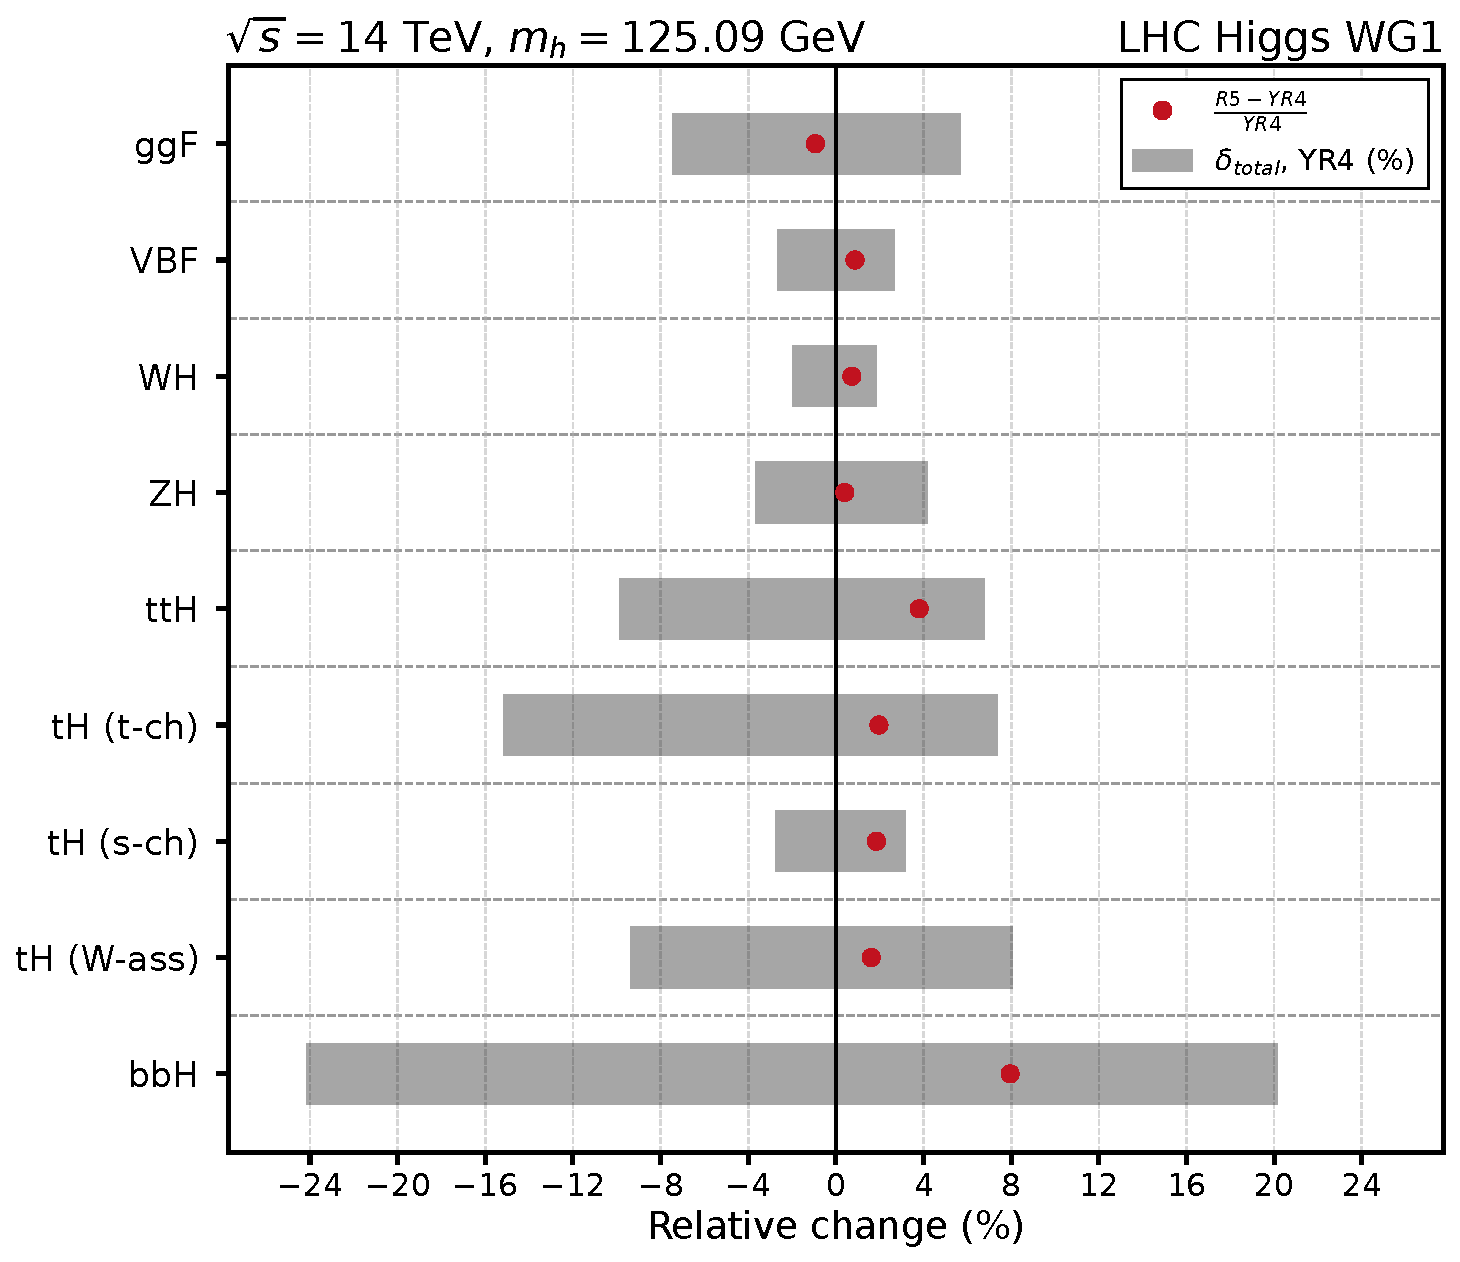
\includegraphics[width=0.95\textwidth]{plots/central_value_comparison.pdf}
    \caption{Change in the central value of the predictions of Higgs boson production cross-sections between the YR4 and R5, relative to the YR4 prediction, for collider energy $\sqrt{s} = 14$ TeV and Higgs boson mass $m_h = 125.09$ GeV. The relative uncertainty on the YR4 prediction is also shown. YR4 predictions for W-associated $tH$ production only exist for $m_h = 125.0$ GeV, so that Higgs mass is used instead.}
    \label{fig:central_values}
\end{figure}

\begin{figure}[!htbp]
    \centering
    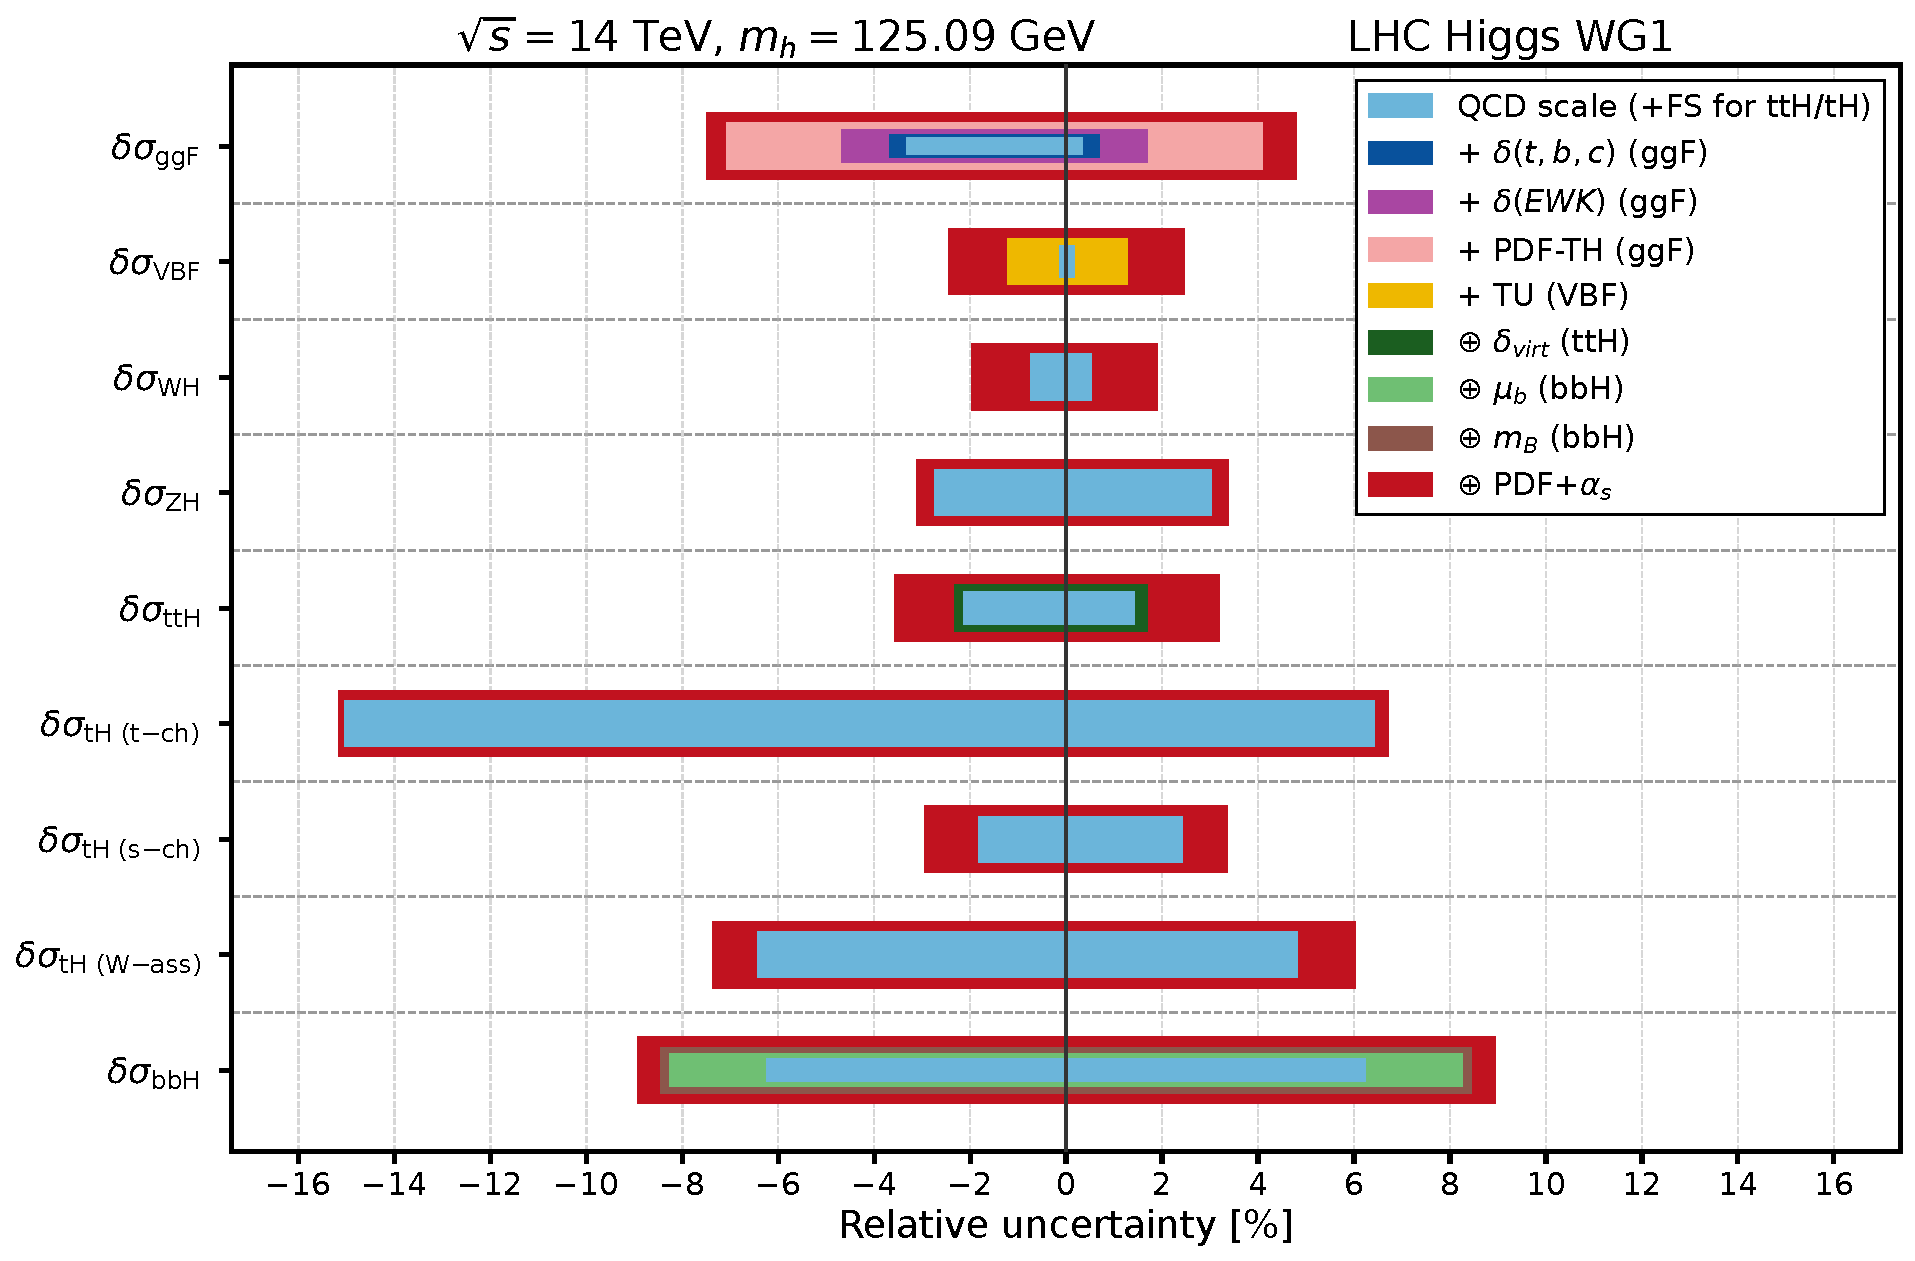
\includegraphics[width=0.95\textwidth]{plots/uncertainty_breakdown_all.pdf}
    \caption{Contribution of various theoretical uncertainties on the Higgs boson production cross sections recommended in this report to the total relative uncertainty. The uncertainties are added one-at-a-time, and the various bars show the total uncertainty after adding each contribution. The symbols in the legend indicate where the source of uncertainty is added linearly ($+$) or in quadrature ($\oplus$).}
    \label{fig:R5_uncertainties_breakdown}
\end{figure}

\begin{figure}[!htbp]
    \centering
    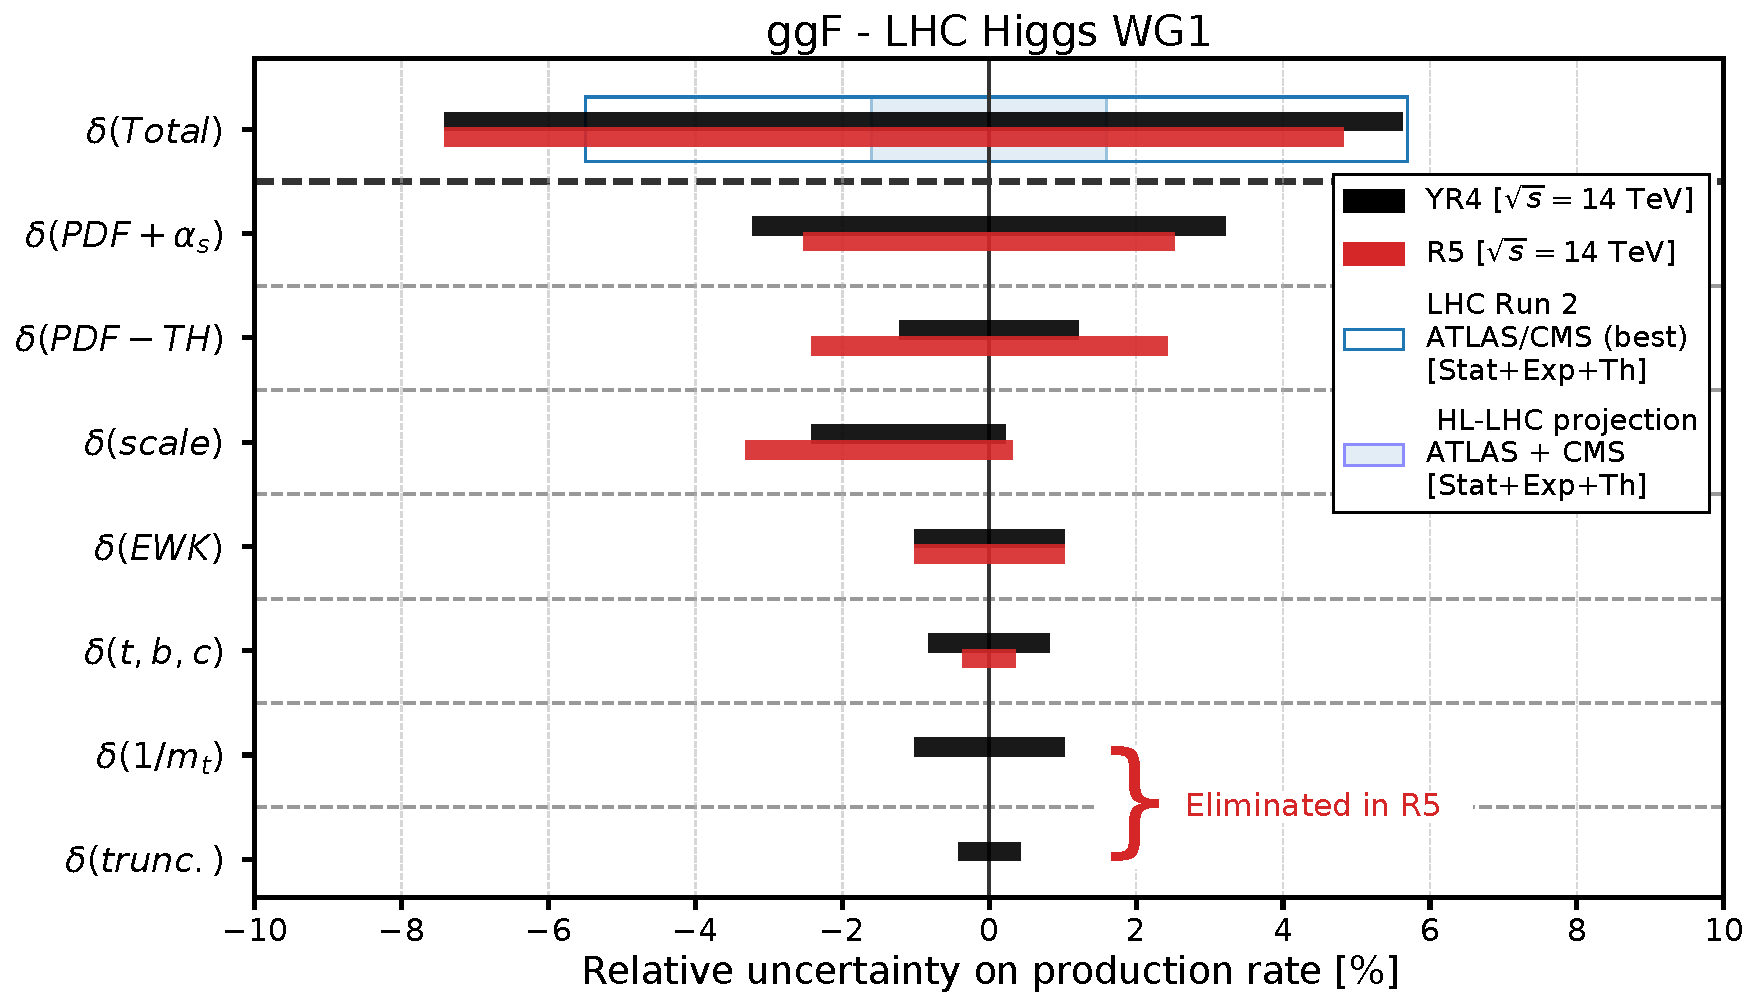
\includegraphics[width=0.95\textwidth]{plots/ggF_uncertainties.pdf}
    \caption{Comparison of the individual contributions to the total theoretical uncertainty on the ggF Higgs boson production cross section recommended in YR4 (black) and in R5 (red). This is compared with the most precise LHC Run 2 Higgs boson signal strength measurement (blue outlined box), whose total uncertainty includes statistical, experimental, and theoretical components, and with the projected HL-LHC ATLAS+CMS combined precision (filled blue box).}
    \label{fig:YR5_ggfsummary_uncertainties}
\end{figure}

Figure~\ref{fig:YR5_summary_uncertainties} expands this comparison by
illustrating the evolution of the theoretical uncertainties on the Higgs
boson production cross-sections between the YR4 and R5 for all production
modes, and compares these results to the precision of measurements of the
Higgs boson production cross-sections at the LHC in Run 2
\cite{ATLAS:2025qxq,CMS:2026nce} and the projected precision of these
measurements at the HL-LHC~\cite{ATLAS:2022hsp}. The corresponding numerical
values are summarised in Table~\ref{tab:prod_uncertainties}. For the ggF,
VBF, ZH and $t\bar t H$ production modes, the anticipated precision of the
measurement at the HL-LHC approaches or exceeds the YR4 theory
precision, illustrating the need for the R5 cross-section update. With the
improved precision of the R5 cross-section predictions, only for ggF does the
projected HL-LHC measurement precision exceed that of the inclusive theory
prediction. Were the optional PDF-theory uncertainty discussed in
Section~\ref{sec:vbf_an3lo} to be included for VBF, bringing its total to
approximately $\pm3.3\%$, the same would become true of VBF. Overall, this
comparison makes clear that the theoretical
advancements brought together in the R5 cross-section predictions are
important for fully exploiting the potential of the HL-LHC. It should also
be noted that the HL-LHC projections themselves assume a reduction by a
factor of two, relative to the YR4, of the theory uncertainties entering the
measurement uncertainty.

Figure~\ref{fig:YR5_summary_uncertainties} also makes clear that the
predictions for most production modes have seen an improvement in theory
precision. For several production modes, the relative uncertainty is reduced
by multiple percentage points; for others, the improvement is more moderate.
It should be noted that for \bbH{}, where the figure shows the largest change
in relative uncertainty, the comparison is made to the YR4 numbers that use
Santander matching, rather than to the updated numbers using
\nlonnllpart{} matching that were released very shortly after the YR4 and
have substantially smaller uncertainties. For all production modes, the
improved precision reflects advances in higher-order calculations,
improvements in PDFs, and refined treatments of theoretical and parametric
uncertainties. To illustrate the potential impact of further improvements in
PDFs, the theory precision without PDF-related uncertainties is also shown
in the figure. For several of the most precisely predicted production modes,
this results in a substantial reduction of the total uncertainty,
demonstrating that PDF-related uncertainties are an important limitation and
that further progress in this area will be crucial ahead of the HL-LHC.

\begin{figure}[!htbp]
    \centering
    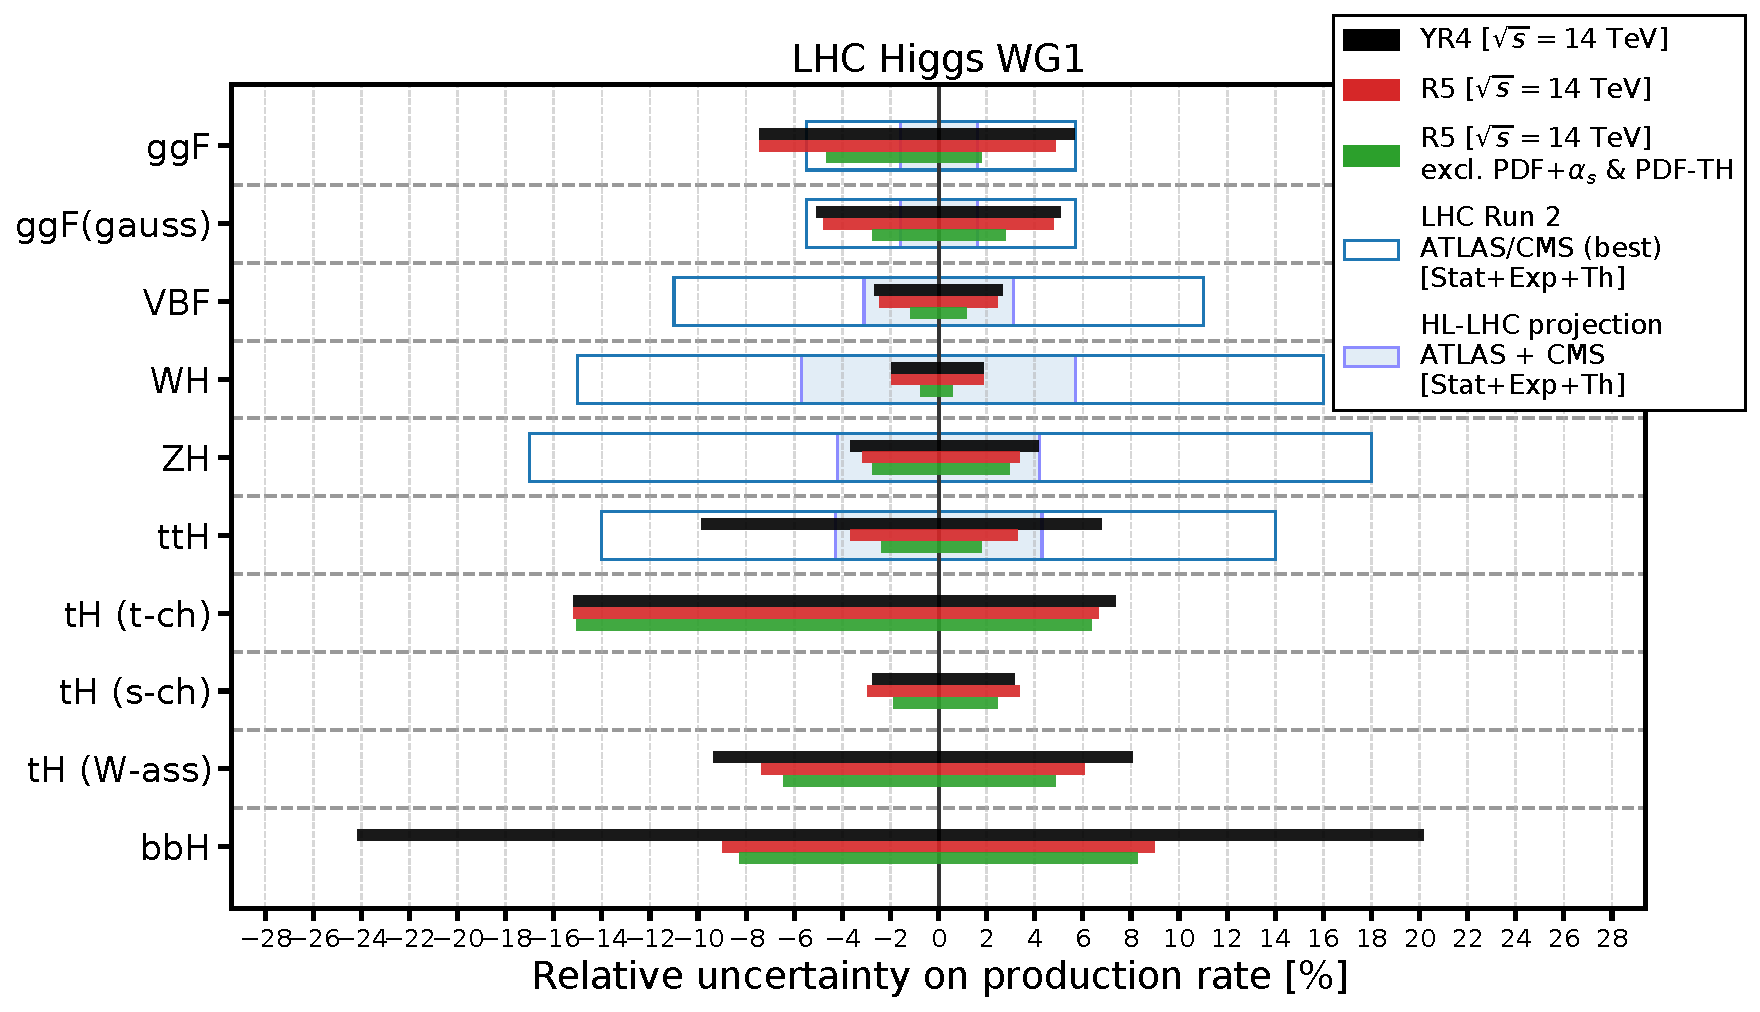
\includegraphics[width=0.95\textwidth]{plots/production_mode_uncertainties.pdf}
    \caption{Comparison of the theoretical uncertainties on the Higgs boson production cross sections recommended in YR4 (black) and in R5 (red) for collider energy $\sqrt{s} = 14$ TeV and Higgs boson mass $m_h = 125.09$ GeV. The current recommendations excluding the PDF$+\alpha_{s}$ and PDF$-$TH contributions are also shown (green). These are compared with the most precise LHC Run 2 Higgs boson signal strength measurements (blue outlined boxes), whose total uncertainties include statistical, experimental, and theoretical components, and with the projected HL-LHC ATLAS+CMS combined precision (filled blue box).}
    \label{fig:YR5_summary_uncertainties}
\end{figure}

\begin{table}[htbp]
\renewcommand{\arraystretch}{1.3}
\setlength{\belowcaptionskip}{10pt}
\centering
\caption{Relative uncertainties (\%) on Higgs boson production cross sections from YR4 and R5, including the R5 uncertainties excluding PDF$+\alpha_{s}$ and PDF$-$TH contributions. These are compared with the most precise LHC Run~2 Higgs boson measurements from ATLAS and CMS, whose total uncertainties include statistical, experimental, and theoretical components, and with the projected HL-LHC ATLAS+CMS combined precision. For the Run~2 measurements and HL-LHC projections, \bbH{} is grouped with ggF and the $tH$ channels are not considered separately, so they are not shown.}
\label{tab:prod_uncertainties}
\begin{tabular}{lccccc}
\toprule
Production mode &
YR4 &
R5 &
R5 (no PDF) &
Run 2 &
HL-LHC \\
\midrule
ggF          & ${}^{+5.6}_{-7.4}$  & ${}^{+4.8}_{-7.4}$  & ${}^{+1.7}_{-4.6}$  & $\pm5.8$           & $\pm1.6$ \\
VBF          & $\pm2.6$            & $\pm2.4$            & $\pm1.1$            & ${}^{+11.7}_{-10.7}$& $\pm3.1$ \\
WH           & ${}^{+1.8}_{-1.9}$  & ${}^{+1.8}_{-1.9}$  & ${}^{+0.5}_{-0.7}$  & $\pm15.6$           & $\pm5.7$ \\
ZH           & ${}^{+4.1}_{-3.6}$  & ${}^{+3.3}_{-3.1}$  & ${}^{+2.9}_{-2.7}$  & ${}^{+17.0}_{-15.6}$& $\pm4.2$ \\
ttH          & ${}^{+6.7}_{-9.8}$  & ${}^{+3.2}_{-3.6}$  & ${}^{+1.7}_{-2.3}$  & ${}^{+23.4}_{-19.4}$& $\pm4.3$ \\
tH ($t$-ch.) & ${}^{+7.3}_{-15.1}$ & ${}^{+6.6}_{-15.1}$ & ${}^{+6.3}_{-15.0}$ & --                  & -- \\
tH ($s$-ch.) & ${}^{+3.1}_{-2.7}$  & ${}^{+3.3}_{-2.9}$  & ${}^{+2.4}_{-1.8}$  & --                  & -- \\
tH ($W$-as)  & ${}^{+8.0}_{-9.3}$  & ${}^{+6.0}_{-7.3}$  & ${}^{+4.8}_{-6.4}$  & --                  & -- \\
bbH          & ${}^{+20.1}_{-24.1}$& ${}^{+8.9}_{-8.9}$  & ${}^{+8.2}_{-8.2}$  & --                  & -- \\
\bottomrule
\end{tabular}
\end{table}

Looking beyond the present recommendations, continued progress in PDF
determinations will be particularly important. Approximate N$^3$LO PDF sets
are already available, and the perturbative ingredients entering N$^3$LO
evolution and matching continue to improve, as discussed in
Section~\ref{sec:an3lo-pdfs}. Establishing a robust common prescription for
PDFs at this accuracy will be important for processes whose hard-scattering
cross sections are already known at N$^3$LO. At the same time, as
percent-level precision becomes increasingly relevant, a more uniform
treatment of QED evolution and photon-initiated contributions will become
desirable. Further progress in higher-order perturbative calculations and
in the assessment of process-specific residual theoretical uncertainties
will remain important for production modes where these effects continue to
limit the prediction.

The recommendations presented in this report represent the current state of
the art. Continued progress in higher-order perturbative calculations, PDF
determinations, and the assessment of residual theoretical uncertainties
will be essential to match the experimental precision expected from the
HL-LHC programme.


\clearpage
%%%%%%%%%%%%%%%%%%%%%%%%%%%%%%%%%%%%%%%%%  Conclusions
\section{Conclusions}
\label{sec:conclusions}
We have presented updated LHC Higgs Working Group recommendations for the
inclusive production cross sections of a Standard Model Higgs boson at
$\sqrt{s}=7,\,8,\,13,\,13.6$ and $14$~TeV and for Higgs-boson masses between
$120$ and $130$~GeV, covering gluon fusion, vector-boson fusion, associated
production with a vector boson, associated production with a top-quark pair or
a single top quark, and associated production with bottom quarks. Within this
scope the report supersedes Yellow Report~4
(YR4)~\cite{LHCHiggsCrossSectionWorkingGroup:2016ypw} and the ad interim
recommendations of Ref.~\cite{Karlberg:2024zxx}, and constitutes the inclusive
cross-section contribution to Report~5 of the working group.

For every production mode the central prediction remains consistent with YR4
within the uncertainties quoted there, while the precision has improved for
most channels. The improvements rest on specific calculations rather than on a
uniform advance: for gluon fusion, the complete N$^3$LO result in the heavy-top
limit~\cite{Mistlberger:2018etf} together with exact NNLO corrections for the
top-only contribution and the top--bottom
interference~\cite{Czakon:2024ywb}; for vector-boson fusion, the N$^3$LO
structure-function result~\cite{Dreyer:2016oyx} supplemented by explicit
calculations of the non-factorisable corrections; for $VH$, the completion of
the NLO QCD corrections to the loop-induced $gg\to ZH$
channel~\cite{CampilloAveleira:2025rbh}; for $t\bar tH$, NNLO QCD matched to
NNLL soft-gluon resummation and combined with the complete NLO electroweak
corrections~\cite{Balsach:2025jcw}; and for $b\bar bH$, the matched
\nlonnllpart{} prediction~\cite{Bonvini:2016fgf}, which carries an explicit
resummation-scale uncertainty. As a consequence the total theoretical
uncertainty, once parton-distribution uncertainties are set aside, is now
smaller than the precision projected for Higgs-boson signal-strength
measurements at the HL-LHC in every channel considered except gluon fusion,
where the projected measurement remains the more precise of the two.

Parton distributions are the binding constraint on further improvement. They
are the leading source of uncertainty in the four most precisely predicted
channels -- gluon fusion, vector-boson fusion, $WH$ and $t\bar tH$ -- where
they account for between roughly a third and three quarters of the total; for
$ZH$, $b\bar bH$ and single-top associated production the residual
perturbative uncertainties dominate instead. The baseline of this
report is PDF4LHC21 at NNLO~\cite{PDF4LHCWorkingGroup:2022cjn}, in line with
the working group's practice of following the PDF4LHC recommendations. Since no
such recommendation exists beyond NNLO, the mismatch between an N$^3$LO matrix
element and NNLO distributions cannot be removed and has instead to be carried
as an uncertainty. How best to estimate that uncertainty proved to depend on
the process. The two independent approximate N$^3$LO determinations agree well
for vector-boson fusion, where they differ by $0.3\%$, but not for gluon
fusion, where they differ by around $3\%$ on an effect of comparable
size~\cite{Cridge:2024icl}. For gluon fusion we have accordingly doubled the
PDF-theory uncertainty relative to YR4, and even that does not fully bracket
the shift; for vector-boson fusion the shift is well determined and comparable
to the uncertainty already assigned, and is quantified but not applied to the
central prediction. Establishing a common prescription for parton distributions
at this accuracy is the single development that would most improve the
predictions collected here.

We have also quantified the effect of QED corrections to the DGLAP evolution,
which shifts the gluon-fusion cross section by up to about $1.7\%$ depending on
the parton distributions and the collider energy, and the vector-boson-fusion
cross section by about $0.6\%$~\cite{Cooper-Sarkar:2025sqw}. The treatment of
QED evolution and of photon-initiated production is not uniform across the
production modes considered here, for reasons of timing set out in
Section~\ref{sec:pdf}, and a uniform treatment is desirable in a future update.

The numerical predictions, together with a full breakdown of the associated
theoretical and parametric uncertainties, are tabulated in
Appendix~\ref{app:tables} for all production modes, collider energies and
Higgs-boson masses considered. The numbers are also available at
\url{https://gitlab.cern.ch/LHCHIGGSXS/LHCHXSWG1/crosssections} together with a set of \texttt{bibtex} citation records of all papers that should be be cited when the cross section predictions from this report are used.\footnote{The numbers in that repository will be updated whenever new results are available for the various production modes. This includes, but is not limited to, updates when a PDF4LHC set becomes available at (a)N$^3$LO. The numbers presented in this report correspond to \texttt{v1.0.1} of the spreadsheet contained in the repository.} We hope that
this report will serve, as YR4 did before it, as the standard reference for
Higgs-boson production cross sections at the LHC and HL-LHC, and we anticipate
that further updates will be required as exact N$^3$LO ingredients, consistent
N$^3$LO parton distributions and refined uncertainty estimates become
available.


%%%%%%%%%%%%%%%%%%%%%%%%%%%%%%%%%%%%%%%%%  Acknowledgments
\section*{Acknowledgments}
This work was done on behalf of the LHCHWG.

G.B. acknowledges partial support from the U.S. Department of Energy, Office of
Science, under Award Number DE-SC0010010.
C.~Biello acknowledges support from the Swiss National Science Foundation under
grant 10001706.
J.C. acknowledges support from the Natural Sciences and Engineering Research
Council of Canada (NSERC).
S.F.R. acknowledges support from the Italian Ministry of Universities and
Research (MUR) under the FIS grant (CUP: D53C24005480001, FLAME).
R.H. acknowledges support from the Dutch Research Council (NWO) under grant
\href{https://doi.org/10.61686/PGEJL69189}{10.61686/PGEJL69189}.
S.J. acknowledges support from the Royal Society under grant URF{\textbackslash}R1{\textbackslash}201268
and from the UK Science and Technology Facilities Council (STFC) under contracts
ST/X000745/1 and ST/X003167/1.
J.M. acknowledges support from the Royal Society under grant
URF{\textbackslash}R1{\textbackslash}201519 and from the STFC under grant ST/W000512/1.
D.M. acknowledges support from MICIU/AEI/10.13039/501100011033/ and ERDF/EU
under grant PID2023-147706NB-I00.
A.M., C.T.P., M.V. and M.~Worek acknowledge support from the Deutsche Forschungsgemeinschaft
(DFG) under grant 396021762 -- TRR 257 ``Particle Physics Phenomenology after the
Higgs Discovery''.
S.Z. acknowledges support from the STFC under grant ST/X000761/1.
M.Z. acknowledges financial support from the Italian Ministry of University and
Research (MUR) through the PRIN2022 grant 2022EZ3S3F, funded by the European
Union -- NextGenerationEU.
L.Z. acknowledges partial support from the U.S. Department of Energy, Office of
Science, under Award Number DE-SC0010072.
\newpage
\appendix
%%%%%%%%%%%%%%%%%%%%%%%%%%%%%%%%%%%%%%%%%  All the tables
\section{Reference tables}
\label{app:tables}
\subsection{ggF}
\begin{landscape}
\begin{table}[ht!]
\caption{Total ggH cross sections in the SM for a LHC CM energy of $\sqrt{s}=7$\,TeV.}
\label{tab:ggH7}
\centering
\scriptsize
{\renewcommand{\arraystretch}{1.4}
\begin{tabular}{| cc | cccc | ccc | c |@{}c@{\;}| cc |@{}c@{\;}| ccc |}
\cline{1-10} \cline{12-13} \cline{15-17}
\multicolumn{2}{|c|}{\(\sqrt{s} = 7\,\mathrm{TeV}\)} &
\multicolumn{4}{l|}{} &
\multicolumn{4}{c|}{NNLO PDF} &
&
\multicolumn{2}{|c|}{aN${}^\text{3}$LO PDF} && \multicolumn{3}{l|}{} \\
%\cline{1-10} \cline{12-13} \cline{15-17}
\(M_\mathrm{H}\,[\mathrm{GeV}]\) & \(\sigma\,[\mathrm{pb}]\) &
\(\delta(\mathrm{theory})\) &
{\color{black!55}\(\delta(\mathrm{scale})\)} & {\color{black!55}\(\delta(\mathrm{EWK})\)} & {\color{black!55}\(\delta(\mathrm{t,b,c})\)} &
\(\delta(\mathrm{PDF}+\alpha_s)\) &
{\color{black!55}\(\delta(\mathrm{PDF})\)} & {\color{black!55}\(\delta(\alpha_s)\)} &
\(\delta(\mathrm{PDF\text{--}TH})\) &
&
\(\Delta\,[\mathrm{pb}]\) & \(\delta(\mathrm{PDF}+\alpha_s)\) & &\(\delta(\mathrm{Gauss})\) & \(\delta(\mathrm{Total})\) & \(\delta(\mathrm{Total(Gauss)})\)
\\
\cline{1-10} \cline{12-13} \cline{15-17}
120.00 & 18.05 & \({}^{ +1.45}_{ -5.05}\%\) & {\color{black!55}\({}^{ +0.11}_{ -3.71}\%\)} & {\color{black!55}\(\pm{  1.00}\%\)} & {\color{black!55}\(\pm{  0.34}\%\)} & \(\pm 2.56\%\) & {\color{black!55}\({}^{ +1.70}_{ -1.70}\%\)} & {\color{black!55}\(\pm 1.92\%\)} & \(\pm{  1.84}\%\) &  & \(-0.97\) & \({}^{ +1.83}_{ -1.83}\%\) &  & \(\pm 3.98\%\) & \({}^{ +4.17}_{ -7.35}\%\) & \(\pm 4.73\%\)\\
122.00 & 17.45 & \({}^{ +1.45}_{ -5.05}\%\) & {\color{black!55}\({}^{ +0.11}_{ -3.71}\%\)} & {\color{black!55}\(\pm{  1.00}\%\)} & {\color{black!55}\(\pm{  0.34}\%\)} & \(\pm 2.57\%\) & {\color{black!55}\({}^{ +1.70}_{ -1.70}\%\)} & {\color{black!55}\(\pm 1.93\%\)} & \(\pm{  1.82}\%\) &  & \(-0.94\) & \({}^{ +1.82}_{ -1.82}\%\) &  & \(\pm 3.97\%\) & \({}^{ +4.16}_{ -7.33}\%\) & \(\pm 4.73\%\)\\
124.00 & 16.88 & \({}^{ +1.45}_{ -5.04}\%\) & {\color{black!55}\({}^{ +0.11}_{ -3.70}\%\)} & {\color{black!55}\(\pm{  1.00}\%\)} & {\color{black!55}\(\pm{  0.34}\%\)} & \(\pm 2.56\%\) & {\color{black!55}\({}^{ +1.70}_{ -1.70}\%\)} & {\color{black!55}\(\pm 1.92\%\)} & \(\pm{  1.80}\%\) &  & \(-0.91\) & \({}^{ +1.81}_{ -1.81}\%\) &  & \(\pm 3.95\%\) & \({}^{ +4.14}_{ -7.30}\%\) & \(\pm 4.71\%\)\\
124.60 & 16.72 & \({}^{ +1.45}_{ -5.03}\%\) & {\color{black!55}\({}^{ +0.11}_{ -3.69}\%\)} & {\color{black!55}\(\pm{  1.00}\%\)} & {\color{black!55}\(\pm{  0.34}\%\)} & \(\pm 2.57\%\) & {\color{black!55}\({}^{ +1.70}_{ -1.70}\%\)} & {\color{black!55}\(\pm 1.93\%\)} & \(\pm{  1.79}\%\) &  & \(-0.90\) & \({}^{ +1.81}_{ -1.81}\%\) &  & \(\pm 3.94\%\) & \({}^{ +4.13}_{ -7.29}\%\) & \(\pm 4.70\%\)\\
124.80 & 16.66 & \({}^{ +1.45}_{ -5.03}\%\) & {\color{black!55}\({}^{ +0.11}_{ -3.69}\%\)} & {\color{black!55}\(\pm{  1.00}\%\)} & {\color{black!55}\(\pm{  0.34}\%\)} & \(\pm 2.57\%\) & {\color{black!55}\({}^{ +1.70}_{ -1.70}\%\)} & {\color{black!55}\(\pm 1.93\%\)} & \(\pm{  1.79}\%\) &  & \(-0.90\) & \({}^{ +1.81}_{ -1.81}\%\) &  & \(\pm 3.94\%\) & \({}^{ +4.13}_{ -7.29}\%\) & \(\pm 4.70\%\)\\
125.00 & 16.61 & \({}^{ +1.45}_{ -5.03}\%\) & {\color{black!55}\({}^{ +0.11}_{ -3.69}\%\)} & {\color{black!55}\(\pm{  1.00}\%\)} & {\color{black!55}\(\pm{  0.34}\%\)} & \(\pm 2.57\%\) & {\color{black!55}\({}^{ +1.70}_{ -1.70}\%\)} & {\color{black!55}\(\pm 1.93\%\)} & \(\pm{  1.79}\%\) &  & \(-0.90\) & \({}^{ +1.81}_{ -1.81}\%\) &  & \(\pm 3.94\%\) & \({}^{ +4.13}_{ -7.29}\%\) & \(\pm 4.70\%\)\\
125.09 & 16.58 & \({}^{ +1.45}_{ -5.03}\%\) & {\color{black!55}\({}^{ +0.11}_{ -3.69}\%\)} & {\color{black!55}\(\pm{  1.00}\%\)} & {\color{black!55}\(\pm{  0.34}\%\)} & \(\pm 2.57\%\) & {\color{black!55}\({}^{ +1.70}_{ -1.70}\%\)} & {\color{black!55}\(\pm 1.93\%\)} & \(\pm{  1.79}\%\) &  & \(-0.89\) & \({}^{ +1.81}_{ -1.81}\%\) &  & \(\pm 3.94\%\) & \({}^{ +4.13}_{ -7.29}\%\) & \(\pm 4.70\%\)\\
125.20 & 16.55 & \({}^{ +1.45}_{ -5.03}\%\) & {\color{black!55}\({}^{ +0.11}_{ -3.69}\%\)} & {\color{black!55}\(\pm{  1.00}\%\)} & {\color{black!55}\(\pm{  0.34}\%\)} & \(\pm 2.57\%\) & {\color{black!55}\({}^{ +1.70}_{ -1.70}\%\)} & {\color{black!55}\(\pm 1.93\%\)} & \(\pm{  1.79}\%\) &  & \(-0.89\) & \({}^{ +1.81}_{ -1.81}\%\) &  & \(\pm 3.94\%\) & \({}^{ +4.13}_{ -7.29}\%\) & \(\pm 4.70\%\)\\
125.30 & 16.53 & \({}^{ +1.45}_{ -5.03}\%\) & {\color{black!55}\({}^{ +0.11}_{ -3.69}\%\)} & {\color{black!55}\(\pm{  1.00}\%\)} & {\color{black!55}\(\pm{  0.34}\%\)} & \(\pm 2.56\%\) & {\color{black!55}\({}^{ +1.70}_{ -1.70}\%\)} & {\color{black!55}\(\pm 1.92\%\)} & \(\pm{  1.79}\%\) &  & \(-0.89\) & \({}^{ +1.81}_{ -1.81}\%\) &  & \(\pm 3.94\%\) & \({}^{ +4.13}_{ -7.29}\%\) & \(\pm 4.70\%\)\\
125.38 & 16.50 & \({}^{ +1.45}_{ -5.03}\%\) & {\color{black!55}\({}^{ +0.11}_{ -3.69}\%\)} & {\color{black!55}\(\pm{  1.00}\%\)} & {\color{black!55}\(\pm{  0.34}\%\)} & \(\pm 2.56\%\) & {\color{black!55}\({}^{ +1.70}_{ -1.70}\%\)} & {\color{black!55}\(\pm 1.92\%\)} & \(\pm{  1.78}\%\) &  & \(-0.89\) & \({}^{ +1.81}_{ -1.81}\%\) &  & \(\pm 3.93\%\) & \({}^{ +4.12}_{ -7.28}\%\) & \(\pm 4.69\%\)\\
125.60 & 16.45 & \({}^{ +1.45}_{ -5.03}\%\) & {\color{black!55}\({}^{ +0.11}_{ -3.69}\%\)} & {\color{black!55}\(\pm{  1.00}\%\)} & {\color{black!55}\(\pm{  0.34}\%\)} & \(\pm 2.56\%\) & {\color{black!55}\({}^{ +1.70}_{ -1.70}\%\)} & {\color{black!55}\(\pm 1.92\%\)} & \(\pm{  1.78}\%\) &  & \(-0.89\) & \({}^{ +1.81}_{ -1.81}\%\) &  & \(\pm 3.93\%\) & \({}^{ +4.12}_{ -7.28}\%\) & \(\pm 4.69\%\)\\
126.00 & 16.34 & \({}^{ +1.45}_{ -5.03}\%\) & {\color{black!55}\({}^{ +0.11}_{ -3.69}\%\)} & {\color{black!55}\(\pm{  1.00}\%\)} & {\color{black!55}\(\pm{  0.34}\%\)} & \(\pm 2.56\%\) & {\color{black!55}\({}^{ +1.70}_{ -1.70}\%\)} & {\color{black!55}\(\pm 1.92\%\)} & \(\pm{  1.78}\%\) &  & \(-0.88\) & \({}^{ +1.81}_{ -1.81}\%\) &  & \(\pm 3.93\%\) & \({}^{ +4.12}_{ -7.28}\%\) & \(\pm 4.69\%\)\\
128.00 & 15.82 & \({}^{ +1.45}_{ -5.03}\%\) & {\color{black!55}\({}^{ +0.11}_{ -3.69}\%\)} & {\color{black!55}\(\pm{  1.00}\%\)} & {\color{black!55}\(\pm{  0.34}\%\)} & \(\pm 2.56\%\) & {\color{black!55}\({}^{ +1.70}_{ -1.70}\%\)} & {\color{black!55}\(\pm 1.92\%\)} & \(\pm{  1.76}\%\) &  & \(-0.85\) & \({}^{ +1.80}_{ -1.80}\%\) &  & \(\pm 3.92\%\) & \({}^{ +4.11}_{ -7.26}\%\) & \(\pm 4.68\%\)\\
130.00 & 15.32 & \({}^{ +1.46}_{ -5.02}\%\) & {\color{black!55}\({}^{ +0.12}_{ -3.68}\%\)} & {\color{black!55}\(\pm{  1.00}\%\)} & {\color{black!55}\(\pm{  0.34}\%\)} & \(\pm 2.56\%\) & {\color{black!55}\({}^{ +1.70}_{ -1.70}\%\)} & {\color{black!55}\(\pm 1.92\%\)} & \(\pm{  1.74}\%\) &  & \(-0.83\) & \({}^{ +1.79}_{ -1.79}\%\) &  & \(\pm 3.90\%\) & \({}^{ +4.10}_{ -7.23}\%\) & \(\pm 4.67\%\)\\
\cline{1-10} \cline{12-13} \cline{15-17}
\end{tabular}
}
\end{table}

\begin{table}[ht!]
\caption{Total ggH cross sections in the SM for a LHC CM energy of $\sqrt{s}=8$\,TeV.}
\label{tab:ggH8}
\centering
\scriptsize
{\renewcommand{\arraystretch}{1.4}
\begin{tabular}{| cc | cccc | ccc | c |@{}c@{\;}| cc |@{}c@{\;}| ccc |}
\cline{1-10} \cline{12-13} \cline{15-17}
\multicolumn{2}{|c|}{\(\sqrt{s} = 8\,\mathrm{TeV}\)} &
\multicolumn{4}{l|}{} &
\multicolumn{4}{c|}{NNLO PDF} &
&
\multicolumn{2}{|c|}{aN${}^\text{3}$LO PDF} && \multicolumn{3}{l|}{} \\
%\cline{1-10} \cline{12-13} \cline{15-17}
\(M_\mathrm{H}\,[\mathrm{GeV}]\) & \(\sigma\,[\mathrm{pb}]\) &
\(\delta(\mathrm{theory})\) &
{\color{black!55}\(\delta(\mathrm{scale})\)} & {\color{black!55}\(\delta(\mathrm{EWK})\)} & {\color{black!55}\(\delta(\mathrm{t,b,c})\)} &
\(\delta(\mathrm{PDF}+\alpha_s)\) &
{\color{black!55}\(\delta(\mathrm{PDF})\)} & {\color{black!55}\(\delta(\alpha_s)\)} &
\(\delta(\mathrm{PDF\text{--}TH})\) &
&
\(\Delta\,[\mathrm{pb}]\) & \(\delta(\mathrm{PDF}+\alpha_s)\) & &\(\delta(\mathrm{Gauss})\) & \(\delta(\mathrm{Total})\) & \(\delta(\mathrm{Total(Gauss)})\)
\\
\cline{1-10} \cline{12-13} \cline{15-17}
120.00 & 22.91 & \({}^{ +1.48}_{ -4.97}\%\) & {\color{black!55}\({}^{ +0.14}_{ -3.63}\%\)} & {\color{black!55}\(\pm{  1.00}\%\)} & {\color{black!55}\(\pm{  0.34}\%\)} & \(\pm 2.54\%\) & {\color{black!55}\({}^{ +1.69}_{ -1.69}\%\)} & {\color{black!55}\(\pm 1.90\%\)} & \(\pm{  1.95}\%\) &  & \(-1.21\) & \({}^{ +1.83}_{ -1.83}\%\) &  & \(\pm 4.00\%\) & \({}^{ +4.27}_{ -7.37}\%\) & \(\pm 4.74\%\)\\
122.00 & 22.18 & \({}^{ +1.49}_{ -4.96}\%\) & {\color{black!55}\({}^{ +0.15}_{ -3.62}\%\)} & {\color{black!55}\(\pm{  1.00}\%\)} & {\color{black!55}\(\pm{  0.34}\%\)} & \(\pm 2.53\%\) & {\color{black!55}\({}^{ +1.68}_{ -1.68}\%\)} & {\color{black!55}\(\pm 1.90\%\)} & \(\pm{  1.93}\%\) &  & \(-1.17\) & \({}^{ +1.83}_{ -1.83}\%\) &  & \(\pm 3.98\%\) & \({}^{ +4.26}_{ -7.34}\%\) & \(\pm 4.72\%\)\\
124.00 & 21.47 & \({}^{ +1.49}_{ -4.95}\%\) & {\color{black!55}\({}^{ +0.15}_{ -3.61}\%\)} & {\color{black!55}\(\pm{  1.00}\%\)} & {\color{black!55}\(\pm{  0.34}\%\)} & \(\pm 2.53\%\) & {\color{black!55}\({}^{ +1.68}_{ -1.68}\%\)} & {\color{black!55}\(\pm 1.90\%\)} & \(\pm{  1.91}\%\) &  & \(-1.13\) & \({}^{ +1.82}_{ -1.82}\%\) &  & \(\pm 3.96\%\) & \({}^{ +4.24}_{ -7.31}\%\) & \(\pm 4.70\%\)\\
124.60 & 21.27 & \({}^{ +1.49}_{ -4.95}\%\) & {\color{black!55}\({}^{ +0.15}_{ -3.61}\%\)} & {\color{black!55}\(\pm{  1.00}\%\)} & {\color{black!55}\(\pm{  0.34}\%\)} & \(\pm 2.53\%\) & {\color{black!55}\({}^{ +1.68}_{ -1.68}\%\)} & {\color{black!55}\(\pm 1.90\%\)} & \(\pm{  1.90}\%\) &  & \(-1.12\) & \({}^{ +1.82}_{ -1.82}\%\) &  & \(\pm 3.95\%\) & \({}^{ +4.23}_{ -7.30}\%\) & \(\pm 4.70\%\)\\
124.80 & 21.20 & \({}^{ +1.49}_{ -4.95}\%\) & {\color{black!55}\({}^{ +0.15}_{ -3.61}\%\)} & {\color{black!55}\(\pm{  1.00}\%\)} & {\color{black!55}\(\pm{  0.34}\%\)} & \(\pm 2.53\%\) & {\color{black!55}\({}^{ +1.68}_{ -1.68}\%\)} & {\color{black!55}\(\pm 1.90\%\)} & \(\pm{  1.90}\%\) &  & \(-1.12\) & \({}^{ +1.82}_{ -1.82}\%\) &  & \(\pm 3.95\%\) & \({}^{ +4.23}_{ -7.30}\%\) & \(\pm 4.70\%\)\\
125.00 & 21.14 & \({}^{ +1.49}_{ -4.95}\%\) & {\color{black!55}\({}^{ +0.15}_{ -3.61}\%\)} & {\color{black!55}\(\pm{  1.00}\%\)} & {\color{black!55}\(\pm{  0.34}\%\)} & \(\pm 2.53\%\) & {\color{black!55}\({}^{ +1.68}_{ -1.68}\%\)} & {\color{black!55}\(\pm 1.90\%\)} & \(\pm{  1.89}\%\) &  & \(-1.11\) & \({}^{ +1.82}_{ -1.82}\%\) &  & \(\pm 3.95\%\) & \({}^{ +4.22}_{ -7.29}\%\) & \(\pm 4.69\%\)\\
125.09 & 21.11 & \({}^{ +1.49}_{ -4.95}\%\) & {\color{black!55}\({}^{ +0.15}_{ -3.61}\%\)} & {\color{black!55}\(\pm{  1.00}\%\)} & {\color{black!55}\(\pm{  0.34}\%\)} & \(\pm 2.53\%\) & {\color{black!55}\({}^{ +1.68}_{ -1.68}\%\)} & {\color{black!55}\(\pm 1.90\%\)} & \(\pm{  1.89}\%\) &  & \(-1.11\) & \({}^{ +1.82}_{ -1.82}\%\) &  & \(\pm 3.95\%\) & \({}^{ +4.22}_{ -7.29}\%\) & \(\pm 4.69\%\)\\
125.20 & 21.07 & \({}^{ +1.49}_{ -4.95}\%\) & {\color{black!55}\({}^{ +0.15}_{ -3.61}\%\)} & {\color{black!55}\(\pm{  1.00}\%\)} & {\color{black!55}\(\pm{  0.34}\%\)} & \(\pm 2.53\%\) & {\color{black!55}\({}^{ +1.68}_{ -1.68}\%\)} & {\color{black!55}\(\pm 1.90\%\)} & \(\pm{  1.89}\%\) &  & \(-1.11\) & \({}^{ +1.82}_{ -1.82}\%\) &  & \(\pm 3.95\%\) & \({}^{ +4.22}_{ -7.29}\%\) & \(\pm 4.69\%\)\\
125.30 & 21.04 & \({}^{ +1.49}_{ -4.95}\%\) & {\color{black!55}\({}^{ +0.15}_{ -3.61}\%\)} & {\color{black!55}\(\pm{  1.00}\%\)} & {\color{black!55}\(\pm{  0.34}\%\)} & \(\pm 2.53\%\) & {\color{black!55}\({}^{ +1.68}_{ -1.68}\%\)} & {\color{black!55}\(\pm 1.90\%\)} & \(\pm{  1.89}\%\) &  & \(-1.11\) & \({}^{ +1.82}_{ -1.82}\%\) &  & \(\pm 3.95\%\) & \({}^{ +4.22}_{ -7.29}\%\) & \(\pm 4.69\%\)\\
125.38 & 21.01 & \({}^{ +1.49}_{ -4.95}\%\) & {\color{black!55}\({}^{ +0.15}_{ -3.61}\%\)} & {\color{black!55}\(\pm{  1.00}\%\)} & {\color{black!55}\(\pm{  0.34}\%\)} & \(\pm 2.53\%\) & {\color{black!55}\({}^{ +1.68}_{ -1.68}\%\)} & {\color{black!55}\(\pm 1.90\%\)} & \(\pm{  1.89}\%\) &  & \(-1.11\) & \({}^{ +1.82}_{ -1.82}\%\) &  & \(\pm 3.95\%\) & \({}^{ +4.22}_{ -7.29}\%\) & \(\pm 4.69\%\)\\
125.60 & 20.94 & \({}^{ +1.49}_{ -4.95}\%\) & {\color{black!55}\({}^{ +0.15}_{ -3.61}\%\)} & {\color{black!55}\(\pm{  1.00}\%\)} & {\color{black!55}\(\pm{  0.34}\%\)} & \(\pm 2.53\%\) & {\color{black!55}\({}^{ +1.68}_{ -1.68}\%\)} & {\color{black!55}\(\pm 1.90\%\)} & \(\pm{  1.89}\%\) &  & \(-1.10\) & \({}^{ +1.82}_{ -1.82}\%\) &  & \(\pm 3.95\%\) & \({}^{ +4.22}_{ -7.29}\%\) & \(\pm 4.69\%\)\\
126.00 & 20.81 & \({}^{ +1.49}_{ -4.95}\%\) & {\color{black!55}\({}^{ +0.15}_{ -3.61}\%\)} & {\color{black!55}\(\pm{  1.00}\%\)} & {\color{black!55}\(\pm{  0.34}\%\)} & \(\pm 2.53\%\) & {\color{black!55}\({}^{ +1.68}_{ -1.68}\%\)} & {\color{black!55}\(\pm 1.89\%\)} & \(\pm{  1.88}\%\) &  & \(-1.10\) & \({}^{ +1.82}_{ -1.82}\%\) &  & \(\pm 3.94\%\) & \({}^{ +4.21}_{ -7.28}\%\) & \(\pm 4.68\%\)\\
128.00 & 20.17 & \({}^{ +1.49}_{ -4.94}\%\) & {\color{black!55}\({}^{ +0.15}_{ -3.60}\%\)} & {\color{black!55}\(\pm{  1.00}\%\)} & {\color{black!55}\(\pm{  0.34}\%\)} & \(\pm 2.53\%\) & {\color{black!55}\({}^{ +1.68}_{ -1.68}\%\)} & {\color{black!55}\(\pm 1.89\%\)} & \(\pm{  1.86}\%\) &  & \(-1.06\) & \({}^{ +1.81}_{ -1.81}\%\) &  & \(\pm 3.93\%\) & \({}^{ +4.20}_{ -7.25}\%\) & \(\pm 4.67\%\)\\
130.00 & 19.56 & \({}^{ +1.48}_{ -4.94}\%\) & {\color{black!55}\({}^{ +0.14}_{ -3.60}\%\)} & {\color{black!55}\(\pm{  1.00}\%\)} & {\color{black!55}\(\pm{  0.34}\%\)} & \(\pm 2.53\%\) & {\color{black!55}\({}^{ +1.68}_{ -1.68}\%\)} & {\color{black!55}\(\pm 1.89\%\)} & \(\pm{  1.84}\%\) &  & \(-1.03\) & \({}^{ +1.81}_{ -1.81}\%\) &  & \(\pm 3.91\%\) & \({}^{ +4.17}_{ -7.24}\%\) & \(\pm 4.66\%\)\\
\cline{1-10} \cline{12-13} \cline{15-17}
\end{tabular}
}
\end{table}

\begin{table}[ht!]
\caption{Total ggH cross sections in the SM for a LHC CM energy of $\sqrt{s}=13$\,TeV.}
\label{tab:ggH13}
\centering
\scriptsize
{\renewcommand{\arraystretch}{1.4}
\begin{tabular}{| cc | cccc | ccc | c |@{}c@{\;}| cc |@{}c@{\;}| ccc |}
\cline{1-10} \cline{12-13} \cline{15-17}
\multicolumn{2}{|c|}{\(\sqrt{s} = 13\,\mathrm{TeV}\)} &
\multicolumn{4}{l|}{} &
\multicolumn{4}{c|}{NNLO PDF} &
&
\multicolumn{2}{|c|}{aN${}^\text{3}$LO PDF} && \multicolumn{3}{l|}{} \\
%\cline{1-10} \cline{12-13} \cline{15-17}
\(M_\mathrm{H}\,[\mathrm{GeV}]\) & \(\sigma\,[\mathrm{pb}]\) &
\(\delta(\mathrm{theory})\) &
{\color{black!55}\(\delta(\mathrm{scale})\)} & {\color{black!55}\(\delta(\mathrm{EWK})\)} & {\color{black!55}\(\delta(\mathrm{t,b,c})\)} &
\(\delta(\mathrm{PDF}+\alpha_s)\) &
{\color{black!55}\(\delta(\mathrm{PDF})\)} & {\color{black!55}\(\delta(\alpha_s)\)} &
\(\delta(\mathrm{PDF\text{--}TH})\) &
&
\(\Delta\,[\mathrm{pb}]\) & \(\delta(\mathrm{PDF}+\alpha_s)\) & &\(\delta(\mathrm{Gauss})\) & \(\delta(\mathrm{Total})\) & \(\delta(\mathrm{Total(Gauss)})\)
\\
\cline{1-10} \cline{12-13} \cline{15-17}
120.00 & 51.67 & \({}^{ +1.64}_{ -4.69}\%\) & {\color{black!55}\({}^{ +0.30}_{ -3.35}\%\)} & {\color{black!55}\(\pm{  1.00}\%\)} & {\color{black!55}\(\pm{  0.34}\%\)} & \(\pm 2.48\%\) & {\color{black!55}\({}^{ +1.65}_{ -1.65}\%\)} & {\color{black!55}\(\pm 1.85\%\)} & \(\pm{  2.38}\%\) &  & \(-2.42\) & \({}^{ +1.75}_{ -1.75}\%\) &  & \(\pm 4.08\%\) & \({}^{ +4.72}_{ -7.49}\%\) & \(\pm 4.77\%\)\\
122.00 & 50.20 & \({}^{ +1.63}_{ -4.68}\%\) & {\color{black!55}\({}^{ +0.29}_{ -3.34}\%\)} & {\color{black!55}\(\pm{  1.00}\%\)} & {\color{black!55}\(\pm{  0.34}\%\)} & \(\pm 2.47\%\) & {\color{black!55}\({}^{ +1.65}_{ -1.65}\%\)} & {\color{black!55}\(\pm 1.84\%\)} & \(\pm{  2.35}\%\) &  & \(-2.35\) & \({}^{ +1.75}_{ -1.75}\%\) &  & \(\pm 4.06\%\) & \({}^{ +4.68}_{ -7.45}\%\) & \(\pm 4.75\%\)\\
124.00 & 48.78 & \({}^{ +1.63}_{ -4.67}\%\) & {\color{black!55}\({}^{ +0.29}_{ -3.33}\%\)} & {\color{black!55}\(\pm{  1.00}\%\)} & {\color{black!55}\(\pm{  0.34}\%\)} & \(\pm 2.47\%\) & {\color{black!55}\({}^{ +1.65}_{ -1.65}\%\)} & {\color{black!55}\(\pm 1.84\%\)} & \(\pm{  2.33}\%\) &  & \(-2.29\) & \({}^{ +1.75}_{ -1.75}\%\) &  & \(\pm 4.04\%\) & \({}^{ +4.67}_{ -7.42}\%\) & \(\pm 4.74\%\)\\
124.60 & 48.37 & \({}^{ +1.63}_{ -4.67}\%\) & {\color{black!55}\({}^{ +0.29}_{ -3.33}\%\)} & {\color{black!55}\(\pm{  1.00}\%\)} & {\color{black!55}\(\pm{  0.34}\%\)} & \(\pm 2.47\%\) & {\color{black!55}\({}^{ +1.65}_{ -1.65}\%\)} & {\color{black!55}\(\pm 1.84\%\)} & \(\pm{  2.32}\%\) &  & \(-2.27\) & \({}^{ +1.75}_{ -1.75}\%\) &  & \(\pm 4.04\%\) & \({}^{ +4.66}_{ -7.41}\%\) & \(\pm 4.73\%\)\\
124.80 & 48.23 & \({}^{ +1.63}_{ -4.67}\%\) & {\color{black!55}\({}^{ +0.29}_{ -3.33}\%\)} & {\color{black!55}\(\pm{  1.00}\%\)} & {\color{black!55}\(\pm{  0.34}\%\)} & \(\pm 2.46\%\) & {\color{black!55}\({}^{ +1.65}_{ -1.65}\%\)} & {\color{black!55}\(\pm 1.83\%\)} & \(\pm{  2.32}\%\) &  & \(-2.27\) & \({}^{ +1.75}_{ -1.75}\%\) &  & \(\pm 4.04\%\) & \({}^{ +4.66}_{ -7.41}\%\) & \(\pm 4.73\%\)\\
125.00 & 48.09 & \({}^{ +1.63}_{ -4.67}\%\) & {\color{black!55}\({}^{ +0.29}_{ -3.33}\%\)} & {\color{black!55}\(\pm{  1.00}\%\)} & {\color{black!55}\(\pm{  0.34}\%\)} & \(\pm 2.46\%\) & {\color{black!55}\({}^{ +1.65}_{ -1.65}\%\)} & {\color{black!55}\(\pm 1.83\%\)} & \(\pm{  2.31}\%\) &  & \(-2.26\) & \({}^{ +1.75}_{ -1.75}\%\) &  & \(\pm 4.03\%\) & \({}^{ +4.65}_{ -7.40}\%\) & \(\pm 4.72\%\)\\
125.09 & 48.03 & \({}^{ +1.63}_{ -4.67}\%\) & {\color{black!55}\({}^{ +0.29}_{ -3.33}\%\)} & {\color{black!55}\(\pm{  1.00}\%\)} & {\color{black!55}\(\pm{  0.34}\%\)} & \(\pm 2.46\%\) & {\color{black!55}\({}^{ +1.65}_{ -1.65}\%\)} & {\color{black!55}\(\pm 1.83\%\)} & \(\pm{  2.31}\%\) &  & \(-2.26\) & \({}^{ +1.75}_{ -1.75}\%\) &  & \(\pm 4.03\%\) & \({}^{ +4.65}_{ -7.40}\%\) & \(\pm 4.72\%\)\\
125.20 & 47.96 & \({}^{ +1.63}_{ -4.67}\%\) & {\color{black!55}\({}^{ +0.29}_{ -3.33}\%\)} & {\color{black!55}\(\pm{  1.00}\%\)} & {\color{black!55}\(\pm{  0.34}\%\)} & \(\pm 2.46\%\) & {\color{black!55}\({}^{ +1.65}_{ -1.65}\%\)} & {\color{black!55}\(\pm 1.83\%\)} & \(\pm{  2.31}\%\) &  & \(-2.25\) & \({}^{ +1.75}_{ -1.75}\%\) &  & \(\pm 4.03\%\) & \({}^{ +4.65}_{ -7.40}\%\) & \(\pm 4.72\%\)\\
125.30 & 47.89 & \({}^{ +1.63}_{ -4.66}\%\) & {\color{black!55}\({}^{ +0.29}_{ -3.32}\%\)} & {\color{black!55}\(\pm{  1.00}\%\)} & {\color{black!55}\(\pm{  0.34}\%\)} & \(\pm 2.46\%\) & {\color{black!55}\({}^{ +1.65}_{ -1.65}\%\)} & {\color{black!55}\(\pm 1.83\%\)} & \(\pm{  2.31}\%\) &  & \(-2.25\) & \({}^{ +1.75}_{ -1.75}\%\) &  & \(\pm 4.02\%\) & \({}^{ +4.65}_{ -7.39}\%\) & \(\pm 4.72\%\)\\
125.38 & 47.84 & \({}^{ +1.63}_{ -4.67}\%\) & {\color{black!55}\({}^{ +0.29}_{ -3.33}\%\)} & {\color{black!55}\(\pm{  1.00}\%\)} & {\color{black!55}\(\pm{  0.34}\%\)} & \(\pm 2.46\%\) & {\color{black!55}\({}^{ +1.65}_{ -1.65}\%\)} & {\color{black!55}\(\pm 1.83\%\)} & \(\pm{  2.31}\%\) &  & \(-2.25\) & \({}^{ +1.75}_{ -1.75}\%\) &  & \(\pm 4.03\%\) & \({}^{ +4.65}_{ -7.40}\%\) & \(\pm 4.72\%\)\\
125.60 & 47.69 & \({}^{ +1.63}_{ -4.66}\%\) & {\color{black!55}\({}^{ +0.29}_{ -3.32}\%\)} & {\color{black!55}\(\pm{  1.00}\%\)} & {\color{black!55}\(\pm{  0.34}\%\)} & \(\pm 2.46\%\) & {\color{black!55}\({}^{ +1.65}_{ -1.65}\%\)} & {\color{black!55}\(\pm 1.83\%\)} & \(\pm{  2.31}\%\) &  & \(-2.24\) & \({}^{ +1.75}_{ -1.75}\%\) &  & \(\pm 4.02\%\) & \({}^{ +4.65}_{ -7.39}\%\) & \(\pm 4.72\%\)\\
126.00 & 47.42 & \({}^{ +1.63}_{ -4.66}\%\) & {\color{black!55}\({}^{ +0.29}_{ -3.32}\%\)} & {\color{black!55}\(\pm{  1.00}\%\)} & {\color{black!55}\(\pm{  0.34}\%\)} & \(\pm 2.46\%\) & {\color{black!55}\({}^{ +1.65}_{ -1.65}\%\)} & {\color{black!55}\(\pm 1.83\%\)} & \(\pm{  2.30}\%\) &  & \(-2.23\) & \({}^{ +1.75}_{ -1.75}\%\) &  & \(\pm 4.02\%\) & \({}^{ +4.64}_{ -7.38}\%\) & \(\pm 4.71\%\)\\
128.00 & 46.12 & \({}^{ +1.62}_{ -4.65}\%\) & {\color{black!55}\({}^{ +0.28}_{ -3.31}\%\)} & {\color{black!55}\(\pm{  1.00}\%\)} & {\color{black!55}\(\pm{  0.34}\%\)} & \(\pm 2.46\%\) & {\color{black!55}\({}^{ +1.64}_{ -1.64}\%\)} & {\color{black!55}\(\pm 1.83\%\)} & \(\pm{  2.28}\%\) &  & \(-2.17\) & \({}^{ +1.75}_{ -1.75}\%\) &  & \(\pm 4.00\%\) & \({}^{ +4.61}_{ -7.35}\%\) & \(\pm 4.70\%\)\\
130.00 & 44.87 & \({}^{ +1.62}_{ -4.65}\%\) & {\color{black!55}\({}^{ +0.28}_{ -3.31}\%\)} & {\color{black!55}\(\pm{  1.00}\%\)} & {\color{black!55}\(\pm{  0.34}\%\)} & \(\pm 2.45\%\) & {\color{black!55}\({}^{ +1.64}_{ -1.64}\%\)} & {\color{black!55}\(\pm 1.82\%\)} & \(\pm{  2.25}\%\) &  & \(-2.12\) & \({}^{ +1.76}_{ -1.76}\%\) &  & \(\pm 3.98\%\) & \({}^{ +4.58}_{ -7.32}\%\) & \(\pm 4.68\%\)\\
\cline{1-10} \cline{12-13} \cline{15-17}
\end{tabular}
}
\end{table}

\begin{table}[ht!]
\caption{Total ggH cross sections in the SM for a LHC CM energy of $\sqrt{s}=13.6$\,TeV.}
\label{tab:ggH136}
\centering
\scriptsize
{\renewcommand{\arraystretch}{1.4}
\begin{tabular}{| cc | cccc | ccc | c |@{}c@{\;}| cc |@{}c@{\;}| ccc |}
\cline{1-10} \cline{12-13} \cline{15-17}
\multicolumn{2}{|c|}{\(\sqrt{s} = 13.6\,\mathrm{TeV}\)} &
\multicolumn{4}{l|}{} &
\multicolumn{4}{c|}{NNLO PDF} &
&
\multicolumn{2}{|c|}{aN${}^\text{3}$LO PDF} && \multicolumn{3}{l|}{} \\
%\cline{1-10} \cline{12-13} \cline{15-17}
\(M_\mathrm{H}\,[\mathrm{GeV}]\) & \(\sigma\,[\mathrm{pb}]\) &
\(\delta(\mathrm{theory})\) &
{\color{black!55}\(\delta(\mathrm{scale})\)} & {\color{black!55}\(\delta(\mathrm{EWK})\)} & {\color{black!55}\(\delta(\mathrm{t,b,c})\)} &
\(\delta(\mathrm{PDF}+\alpha_s)\) &
{\color{black!55}\(\delta(\mathrm{PDF})\)} & {\color{black!55}\(\delta(\alpha_s)\)} &
\(\delta(\mathrm{PDF\text{--}TH})\) &
&
\(\Delta\,[\mathrm{pb}]\) & \(\delta(\mathrm{PDF}+\alpha_s)\) & &\(\delta(\mathrm{Gauss})\) & \(\delta(\mathrm{Total})\) & \(\delta(\mathrm{Total(Gauss)})\)
\\
\cline{1-10} \cline{12-13} \cline{15-17}
120.00 & 55.54 & \({}^{ +1.65}_{ -4.66}\%\) & {\color{black!55}\({}^{ +0.31}_{ -3.32}\%\)} & {\color{black!55}\(\pm{  1.00}\%\)} & {\color{black!55}\(\pm{  0.34}\%\)} & \(\pm 2.48\%\) & {\color{black!55}\({}^{ +1.65}_{ -1.65}\%\)} & {\color{black!55}\(\pm 1.85\%\)} & \(\pm{  2.42}\%\) &  & \(-2.56\) & \({}^{ +1.73}_{ -1.73}\%\) &  & \(\pm 4.09\%\) & \({}^{ +4.76}_{ -7.50}\%\) & \(\pm 4.78\%\)\\
122.00 & 53.97 & \({}^{ +1.66}_{ -4.65}\%\) & {\color{black!55}\({}^{ +0.32}_{ -3.31}\%\)} & {\color{black!55}\(\pm{  1.00}\%\)} & {\color{black!55}\(\pm{  0.34}\%\)} & \(\pm 2.47\%\) & {\color{black!55}\({}^{ +1.65}_{ -1.65}\%\)} & {\color{black!55}\(\pm 1.84\%\)} & \(\pm{  2.40}\%\) &  & \(-2.49\) & \({}^{ +1.73}_{ -1.73}\%\) &  & \(\pm 4.07\%\) & \({}^{ +4.75}_{ -7.47}\%\) & \(\pm 4.76\%\)\\
124.00 & 52.46 & \({}^{ +1.65}_{ -4.65}\%\) & {\color{black!55}\({}^{ +0.31}_{ -3.31}\%\)} & {\color{black!55}\(\pm{  1.00}\%\)} & {\color{black!55}\(\pm{  0.34}\%\)} & \(\pm 2.46\%\) & {\color{black!55}\({}^{ +1.64}_{ -1.64}\%\)} & {\color{black!55}\(\pm 1.84\%\)} & \(\pm{  2.37}\%\) &  & \(-2.43\) & \({}^{ +1.74}_{ -1.74}\%\) &  & \(\pm 4.05\%\) & \({}^{ +4.71}_{ -7.44}\%\) & \(\pm 4.74\%\)\\
124.60 & 52.02 & \({}^{ +1.65}_{ -4.65}\%\) & {\color{black!55}\({}^{ +0.31}_{ -3.31}\%\)} & {\color{black!55}\(\pm{  1.00}\%\)} & {\color{black!55}\(\pm{  0.34}\%\)} & \(\pm 2.46\%\) & {\color{black!55}\({}^{ +1.64}_{ -1.64}\%\)} & {\color{black!55}\(\pm 1.84\%\)} & \(\pm{  2.36}\%\) &  & \(-2.41\) & \({}^{ +1.74}_{ -1.74}\%\) &  & \(\pm 4.05\%\) & \({}^{ +4.70}_{ -7.43}\%\) & \(\pm 4.74\%\)\\
124.80 & 51.87 & \({}^{ +1.65}_{ -4.65}\%\) & {\color{black!55}\({}^{ +0.31}_{ -3.31}\%\)} & {\color{black!55}\(\pm{  1.00}\%\)} & {\color{black!55}\(\pm{  0.34}\%\)} & \(\pm 2.46\%\) & {\color{black!55}\({}^{ +1.64}_{ -1.64}\%\)} & {\color{black!55}\(\pm 1.83\%\)} & \(\pm{  2.36}\%\) &  & \(-2.41\) & \({}^{ +1.74}_{ -1.74}\%\) &  & \(\pm 4.05\%\) & \({}^{ +4.70}_{ -7.43}\%\) & \(\pm 4.73\%\)\\
125.00 & 51.72 & \({}^{ +1.65}_{ -4.65}\%\) & {\color{black!55}\({}^{ +0.31}_{ -3.31}\%\)} & {\color{black!55}\(\pm{  1.00}\%\)} & {\color{black!55}\(\pm{  0.34}\%\)} & \(\pm 2.46\%\) & {\color{black!55}\({}^{ +1.64}_{ -1.64}\%\)} & {\color{black!55}\(\pm 1.83\%\)} & \(\pm{  2.36}\%\) &  & \(-2.40\) & \({}^{ +1.74}_{ -1.74}\%\) &  & \(\pm 4.05\%\) & \({}^{ +4.70}_{ -7.43}\%\) & \(\pm 4.73\%\)\\
125.09 & 51.66 & \({}^{ +1.65}_{ -4.65}\%\) & {\color{black!55}\({}^{ +0.31}_{ -3.31}\%\)} & {\color{black!55}\(\pm{  1.00}\%\)} & {\color{black!55}\(\pm{  0.34}\%\)} & \(\pm 2.46\%\) & {\color{black!55}\({}^{ +1.64}_{ -1.64}\%\)} & {\color{black!55}\(\pm 1.83\%\)} & \(\pm{  2.36}\%\) &  & \(-2.40\) & \({}^{ +1.74}_{ -1.74}\%\) &  & \(\pm 4.05\%\) & \({}^{ +4.70}_{ -7.43}\%\) & \(\pm 4.73\%\)\\
125.20 & 51.58 & \({}^{ +1.65}_{ -4.65}\%\) & {\color{black!55}\({}^{ +0.31}_{ -3.31}\%\)} & {\color{black!55}\(\pm{  1.00}\%\)} & {\color{black!55}\(\pm{  0.34}\%\)} & \(\pm 2.46\%\) & {\color{black!55}\({}^{ +1.64}_{ -1.64}\%\)} & {\color{black!55}\(\pm 1.83\%\)} & \(\pm{  2.35}\%\) &  & \(-2.39\) & \({}^{ +1.74}_{ -1.74}\%\) &  & \(\pm 4.04\%\) & \({}^{ +4.69}_{ -7.42}\%\) & \(\pm 4.73\%\)\\
125.30 & 51.51 & \({}^{ +1.65}_{ -4.64}\%\) & {\color{black!55}\({}^{ +0.31}_{ -3.30}\%\)} & {\color{black!55}\(\pm{  1.00}\%\)} & {\color{black!55}\(\pm{  0.34}\%\)} & \(\pm 2.46\%\) & {\color{black!55}\({}^{ +1.64}_{ -1.64}\%\)} & {\color{black!55}\(\pm 1.83\%\)} & \(\pm{  2.35}\%\) &  & \(-2.39\) & \({}^{ +1.74}_{ -1.74}\%\) &  & \(\pm 4.04\%\) & \({}^{ +4.69}_{ -7.41}\%\) & \(\pm 4.72\%\)\\
125.38 & 51.45 & \({}^{ +1.65}_{ -4.64}\%\) & {\color{black!55}\({}^{ +0.31}_{ -3.30}\%\)} & {\color{black!55}\(\pm{  1.00}\%\)} & {\color{black!55}\(\pm{  0.34}\%\)} & \(\pm 2.46\%\) & {\color{black!55}\({}^{ +1.64}_{ -1.64}\%\)} & {\color{black!55}\(\pm 1.83\%\)} & \(\pm{  2.35}\%\) &  & \(-2.39\) & \({}^{ +1.74}_{ -1.74}\%\) &  & \(\pm 4.04\%\) & \({}^{ +4.69}_{ -7.41}\%\) & \(\pm 4.72\%\)\\
125.60 & 51.29 & \({}^{ +1.65}_{ -4.64}\%\) & {\color{black!55}\({}^{ +0.31}_{ -3.30}\%\)} & {\color{black!55}\(\pm{  1.00}\%\)} & {\color{black!55}\(\pm{  0.34}\%\)} & \(\pm 2.46\%\) & {\color{black!55}\({}^{ +1.64}_{ -1.64}\%\)} & {\color{black!55}\(\pm 1.83\%\)} & \(\pm{  2.35}\%\) &  & \(-2.38\) & \({}^{ +1.74}_{ -1.74}\%\) &  & \(\pm 4.04\%\) & \({}^{ +4.69}_{ -7.41}\%\) & \(\pm 4.72\%\)\\
126.00 & 51.01 & \({}^{ +1.65}_{ -4.64}\%\) & {\color{black!55}\({}^{ +0.31}_{ -3.30}\%\)} & {\color{black!55}\(\pm{  1.00}\%\)} & {\color{black!55}\(\pm{  0.34}\%\)} & \(\pm 2.46\%\) & {\color{black!55}\({}^{ +1.64}_{ -1.64}\%\)} & {\color{black!55}\(\pm 1.83\%\)} & \(\pm{  2.34}\%\) &  & \(-2.37\) & \({}^{ +1.74}_{ -1.74}\%\) &  & \(\pm 4.03\%\) & \({}^{ +4.69}_{ -7.40}\%\) & \(\pm 4.72\%\)\\
128.00 & 49.62 & \({}^{ +1.64}_{ -4.63}\%\) & {\color{black!55}\({}^{ +0.30}_{ -3.29}\%\)} & {\color{black!55}\(\pm{  1.00}\%\)} & {\color{black!55}\(\pm{  0.34}\%\)} & \(\pm 2.45\%\) & {\color{black!55}\({}^{ +1.64}_{ -1.64}\%\)} & {\color{black!55}\(\pm 1.83\%\)} & \(\pm{  2.32}\%\) &  & \(-2.31\) & \({}^{ +1.74}_{ -1.74}\%\) &  & \(\pm 4.01\%\) & \({}^{ +4.66}_{ -7.37}\%\) & \(\pm 4.70\%\)\\
130.00 & 48.28 & \({}^{ +1.64}_{ -4.62}\%\) & {\color{black!55}\({}^{ +0.30}_{ -3.28}\%\)} & {\color{black!55}\(\pm{  1.00}\%\)} & {\color{black!55}\(\pm{  0.34}\%\)} & \(\pm 2.45\%\) & {\color{black!55}\({}^{ +1.64}_{ -1.64}\%\)} & {\color{black!55}\(\pm 1.82\%\)} & \(\pm{  2.30}\%\) &  & \(-2.25\) & \({}^{ +1.74}_{ -1.74}\%\) &  & \(\pm 4.00\%\) & \({}^{ +4.64}_{ -7.34}\%\) & \(\pm 4.69\%\)\\
\cline{1-10} \cline{12-13} \cline{15-17}
\end{tabular}
}
\end{table}

\begin{table}[ht!]
\caption{Total ggH cross sections in the SM for a LHC CM energy of $\sqrt{s}=14$\,TeV.}
\label{tab:ggH14}
\centering
\scriptsize
{\renewcommand{\arraystretch}{1.4}
\begin{tabular}{| cc | cccc | ccc | c |@{}c@{\;}| cc |@{}c@{\;}| ccc |}
\cline{1-10} \cline{12-13} \cline{15-17}
\multicolumn{2}{|c|}{\(\sqrt{s} = 14\,\mathrm{TeV}\)} &
\multicolumn{4}{l|}{} &
\multicolumn{4}{c|}{NNLO PDF} &
&
\multicolumn{2}{|c|}{aN${}^\text{3}$LO PDF} && \multicolumn{3}{l|}{} \\
%\cline{1-10} \cline{12-13} \cline{15-17}
\(M_\mathrm{H}\,[\mathrm{GeV}]\) & \(\sigma\,[\mathrm{pb}]\) &
\(\delta(\mathrm{theory})\) &
{\color{black!55}\(\delta(\mathrm{scale})\)} & {\color{black!55}\(\delta(\mathrm{EWK})\)} & {\color{black!55}\(\delta(\mathrm{t,b,c})\)} &
\(\delta(\mathrm{PDF}+\alpha_s)\) &
{\color{black!55}\(\delta(\mathrm{PDF})\)} & {\color{black!55}\(\delta(\alpha_s)\)} &
\(\delta(\mathrm{PDF\text{--}TH})\) &
&
\(\Delta\,[\mathrm{pb}]\) & \(\delta(\mathrm{PDF}+\alpha_s)\) & &\(\delta(\mathrm{Gauss})\) & \(\delta(\mathrm{Total})\) & \(\delta(\mathrm{Total(Gauss)})\)
\\
\cline{1-10} \cline{12-13} \cline{15-17}
120.00 & 58.13 & \({}^{ +1.66}_{ -4.65}\%\) & {\color{black!55}\({}^{ +0.32}_{ -3.31}\%\)} & {\color{black!55}\(\pm{  1.00}\%\)} & {\color{black!55}\(\pm{  0.34}\%\)} & \(\pm 2.47\%\) & {\color{black!55}\({}^{ +1.65}_{ -1.65}\%\)} & {\color{black!55}\(\pm 1.84\%\)} & \(\pm{  2.45}\%\) &  & \(-2.66\) & \({}^{ +1.72}_{ -1.72}\%\) &  & \(\pm 4.10\%\) & \({}^{ +4.80}_{ -7.52}\%\) & \(\pm 4.79\%\)\\
122.00 & 56.50 & \({}^{ +1.66}_{ -4.64}\%\) & {\color{black!55}\({}^{ +0.32}_{ -3.30}\%\)} & {\color{black!55}\(\pm{  1.00}\%\)} & {\color{black!55}\(\pm{  0.34}\%\)} & \(\pm 2.47\%\) & {\color{black!55}\({}^{ +1.65}_{ -1.65}\%\)} & {\color{black!55}\(\pm 1.84\%\)} & \(\pm{  2.42}\%\) &  & \(-2.59\) & \({}^{ +1.72}_{ -1.72}\%\) &  & \(\pm 4.08\%\) & \({}^{ +4.77}_{ -7.48}\%\) & \(\pm 4.76\%\)\\
124.00 & 54.92 & \({}^{ +1.66}_{ -4.63}\%\) & {\color{black!55}\({}^{ +0.32}_{ -3.29}\%\)} & {\color{black!55}\(\pm{  1.00}\%\)} & {\color{black!55}\(\pm{  0.34}\%\)} & \(\pm 2.46\%\) & {\color{black!55}\({}^{ +1.64}_{ -1.64}\%\)} & {\color{black!55}\(\pm 1.84\%\)} & \(\pm{  2.40}\%\) &  & \(-2.52\) & \({}^{ +1.73}_{ -1.73}\%\) &  & \(\pm 4.06\%\) & \({}^{ +4.75}_{ -7.45}\%\) & \(\pm 4.75\%\)\\
124.60 & 54.46 & \({}^{ +1.66}_{ -4.63}\%\) & {\color{black!55}\({}^{ +0.32}_{ -3.29}\%\)} & {\color{black!55}\(\pm{  1.00}\%\)} & {\color{black!55}\(\pm{  0.34}\%\)} & \(\pm 2.46\%\) & {\color{black!55}\({}^{ +1.64}_{ -1.64}\%\)} & {\color{black!55}\(\pm 1.84\%\)} & \(\pm{  2.39}\%\) &  & \(-2.51\) & \({}^{ +1.73}_{ -1.73}\%\) &  & \(\pm 4.05\%\) & \({}^{ +4.74}_{ -7.44}\%\) & \(\pm 4.74\%\)\\
124.80 & 54.31 & \({}^{ +1.66}_{ -4.63}\%\) & {\color{black!55}\({}^{ +0.32}_{ -3.29}\%\)} & {\color{black!55}\(\pm{  1.00}\%\)} & {\color{black!55}\(\pm{  0.34}\%\)} & \(\pm 2.46\%\) & {\color{black!55}\({}^{ +1.64}_{ -1.64}\%\)} & {\color{black!55}\(\pm 1.84\%\)} & \(\pm{  2.39}\%\) &  & \(-2.50\) & \({}^{ +1.73}_{ -1.73}\%\) &  & \(\pm 4.05\%\) & \({}^{ +4.74}_{ -7.44}\%\) & \(\pm 4.74\%\)\\
125.00 & 54.16 & \({}^{ +1.66}_{ -4.63}\%\) & {\color{black!55}\({}^{ +0.32}_{ -3.29}\%\)} & {\color{black!55}\(\pm{  1.00}\%\)} & {\color{black!55}\(\pm{  0.34}\%\)} & \(\pm 2.46\%\) & {\color{black!55}\({}^{ +1.64}_{ -1.64}\%\)} & {\color{black!55}\(\pm 1.83\%\)} & \(\pm{  2.39}\%\) &  & \(-2.49\) & \({}^{ +1.73}_{ -1.73}\%\) &  & \(\pm 4.05\%\) & \({}^{ +4.74}_{ -7.44}\%\) & \(\pm 4.74\%\)\\
125.09 & 54.09 & \({}^{ +1.66}_{ -4.63}\%\) & {\color{black!55}\({}^{ +0.32}_{ -3.29}\%\)} & {\color{black!55}\(\pm{  1.00}\%\)} & {\color{black!55}\(\pm{  0.34}\%\)} & \(\pm 2.46\%\) & {\color{black!55}\({}^{ +1.64}_{ -1.64}\%\)} & {\color{black!55}\(\pm 1.83\%\)} & \(\pm{  2.38}\%\) &  & \(-2.49\) & \({}^{ +1.73}_{ -1.73}\%\) &  & \(\pm 4.05\%\) & \({}^{ +4.73}_{ -7.43}\%\) & \(\pm 4.73\%\)\\
125.20 & 54.01 & \({}^{ +1.66}_{ -4.63}\%\) & {\color{black!55}\({}^{ +0.32}_{ -3.29}\%\)} & {\color{black!55}\(\pm{  1.00}\%\)} & {\color{black!55}\(\pm{  0.34}\%\)} & \(\pm 2.46\%\) & {\color{black!55}\({}^{ +1.64}_{ -1.64}\%\)} & {\color{black!55}\(\pm 1.83\%\)} & \(\pm{  2.38}\%\) &  & \(-2.49\) & \({}^{ +1.73}_{ -1.73}\%\) &  & \(\pm 4.05\%\) & \({}^{ +4.73}_{ -7.43}\%\) & \(\pm 4.73\%\)\\
125.30 & 53.93 & \({}^{ +1.66}_{ -4.63}\%\) & {\color{black!55}\({}^{ +0.32}_{ -3.29}\%\)} & {\color{black!55}\(\pm{  1.00}\%\)} & {\color{black!55}\(\pm{  0.34}\%\)} & \(\pm 2.46\%\) & {\color{black!55}\({}^{ +1.64}_{ -1.64}\%\)} & {\color{black!55}\(\pm 1.83\%\)} & \(\pm{  2.38}\%\) &  & \(-2.48\) & \({}^{ +1.73}_{ -1.73}\%\) &  & \(\pm 4.05\%\) & \({}^{ +4.73}_{ -7.43}\%\) & \(\pm 4.73\%\)\\
125.38 & 53.87 & \({}^{ +1.66}_{ -4.62}\%\) & {\color{black!55}\({}^{ +0.32}_{ -3.28}\%\)} & {\color{black!55}\(\pm{  1.00}\%\)} & {\color{black!55}\(\pm{  0.34}\%\)} & \(\pm 2.46\%\) & {\color{black!55}\({}^{ +1.64}_{ -1.64}\%\)} & {\color{black!55}\(\pm 1.83\%\)} & \(\pm{  2.38}\%\) &  & \(-2.48\) & \({}^{ +1.73}_{ -1.73}\%\) &  & \(\pm 4.04\%\) & \({}^{ +4.73}_{ -7.42}\%\) & \(\pm 4.73\%\)\\
125.60 & 53.71 & \({}^{ +1.66}_{ -4.62}\%\) & {\color{black!55}\({}^{ +0.32}_{ -3.28}\%\)} & {\color{black!55}\(\pm{  1.00}\%\)} & {\color{black!55}\(\pm{  0.34}\%\)} & \(\pm 2.46\%\) & {\color{black!55}\({}^{ +1.64}_{ -1.64}\%\)} & {\color{black!55}\(\pm 1.83\%\)} & \(\pm{  2.38}\%\) &  & \(-2.47\) & \({}^{ +1.73}_{ -1.73}\%\) &  & \(\pm 4.04\%\) & \({}^{ +4.73}_{ -7.42}\%\) & \(\pm 4.73\%\)\\
126.00 & 53.41 & \({}^{ +1.66}_{ -4.62}\%\) & {\color{black!55}\({}^{ +0.32}_{ -3.28}\%\)} & {\color{black!55}\(\pm{  1.00}\%\)} & {\color{black!55}\(\pm{  0.34}\%\)} & \(\pm 2.45\%\) & {\color{black!55}\({}^{ +1.64}_{ -1.64}\%\)} & {\color{black!55}\(\pm 1.83\%\)} & \(\pm{  2.37}\%\) &  & \(-2.46\) & \({}^{ +1.73}_{ -1.73}\%\) &  & \(\pm 4.04\%\) & \({}^{ +4.72}_{ -7.41}\%\) & \(\pm 4.72\%\)\\
128.00 & 51.96 & \({}^{ +1.65}_{ -4.62}\%\) & {\color{black!55}\({}^{ +0.31}_{ -3.28}\%\)} & {\color{black!55}\(\pm{  1.00}\%\)} & {\color{black!55}\(\pm{  0.34}\%\)} & \(\pm 2.45\%\) & {\color{black!55}\({}^{ +1.64}_{ -1.64}\%\)} & {\color{black!55}\(\pm 1.83\%\)} & \(\pm{  2.35}\%\) &  & \(-2.40\) & \({}^{ +1.73}_{ -1.73}\%\) &  & \(\pm 4.02\%\) & \({}^{ +4.69}_{ -7.39}\%\) & \(\pm 4.71\%\)\\
130.00 & 50.58 & \({}^{ +1.65}_{ -4.61}\%\) & {\color{black!55}\({}^{ +0.31}_{ -3.27}\%\)} & {\color{black!55}\(\pm{  1.00}\%\)} & {\color{black!55}\(\pm{  0.34}\%\)} & \(\pm 2.45\%\) & {\color{black!55}\({}^{ +1.64}_{ -1.64}\%\)} & {\color{black!55}\(\pm 1.82\%\)} & \(\pm{  2.32}\%\) &  & \(-2.34\) & \({}^{ +1.73}_{ -1.73}\%\) &  & \(\pm 4.00\%\) & \({}^{ +4.67}_{ -7.35}\%\) & \(\pm 4.69\%\)\\
\cline{1-10} \cline{12-13} \cline{15-17}
\end{tabular}
}
\end{table}

\end{landscape}

\subsection{VBF}
\begin{landscape}
\begin{table}[ht!]
\caption{Total VBF cross sections in the SM for a LHC CM energy of $\sqrt{s}=7$ TeV, including QCD and EW corrections
and their uncertainties for different Higgs-boson masses \texorpdfstring{$\MH$}\MH. 
The cross sections $\sigma_{\NNNLO}^{\DIS}$, $\sigma_{\gamma}$, $\sigma_{\mbox{\scriptsize nf}}$, $\sigma_{\mbox{\scriptsize s/t/u}}$ refer to the NNNLO QCD cross section in the DIS approximation, the photon-induced contributions, the non-factorisable corrections, and the interference between the $s$, $t$, and $u$ diagrams, respectively.
The corrections $\delta_{\ELWK}$ represent the EW corrections excluding the photon-induced contributions.
The uncertainties $\Delta_{\mathrm{PDF}/\alphas/\mathrm{PDF\oplus\alphas}}$ refer to the PDF uncertainty, uncertainty related to the strong coupling, and the quadratically combined uncertainty.
For more details see Section~\ref{sec:VBF}. The uncertainty $\Delta_{\mathrm{theory}}$ is the linear sum of the scale and $\Delta_{\mathrm{TU}}$ uncertainties, separately in the up and down directions.}
\label{tab:vbf_XStot_7}
\centering
\scriptsize
{\renewcommand{\arraystretch}{1.4}
\begin{tabular}{| cc | ccc | ccc | ccc | cc | c |}
\cline{1-14}
\multicolumn{2}{|c|}{\(\sqrt{s} = 7\,\mathrm{TeV}\)} &
\multicolumn{3}{|c|}{Theory uncertainty} &
\multicolumn{3}{|c|}{Parametric uncertainty} &
\multicolumn{5}{|c|}{Cross-section decomposition} &
\multicolumn{1}{c|}{Total uncertainty} \\
\(\MH\,[\mathrm{GeV}]\) & \(\sigma^{\VBF}\,[\mathrm{fb}]\) &
\(\Delta_{\rm theory}\) &
{\color{black!55}\(\Delta_{\rm scale}\)} & {\color{black!55}\(\Delta_{\rm TU}\)} &
\(\Delta_{\rm PDF\oplus\alphas}\) &
{\color{black!55}\(\Delta_{\rm PDF}\)} & {\color{black!55}\(\Delta_{\alphas}\)} &
\(\sigma_{\NNNLO}^{\DIS}\,[\mathrm{fb}]\) & \(\delta_{\ELWK}\,[\%]\) & \(\sigma_\gamma\,[\mathrm{fb}]\) & \(\sigma_{\mathrm{nf}}\,[\mathrm{fb}]\) & \(\sigma_{s/t/u}\,[\mathrm{fb}]\) &
\(\Delta_{\rm total}\)
\\
\cline{1-14}
$120.00$ & $1310$ & $^{+1.1}_{-1.1}\%$ & {\color{black!55}$^{+0.067}_{-0.050}\%$} & {\color{black!55}$\pm 1.0\%$} & $\pm 2.3\%$ & {\color{black!55}$\pm 2.3\%$} & {\color{black!55}$\pm 0.3\%$} & $1360$ & $-4.4\%$ & $9.7$ & $-$ & $-5.3$ & $^{+2.6}_{-2.6}\%$ \\
$122.00$ & $1285$ & $^{+1.1}_{-1.1}\%$ & {\color{black!55}$^{+0.065}_{-0.051}\%$} & {\color{black!55}$\pm 1.0\%$} & $\pm 2.3\%$ & {\color{black!55}$\pm 2.3\%$} & {\color{black!55}$\pm 0.3\%$} & $1333$ & $-4.4\%$ & $9.6$ & $-$ & $-5.0$ & $^{+2.6}_{-2.6}\%$ \\
$124.00$ & $1261$ & $^{+1.1}_{-1.1}\%$ & {\color{black!55}$^{+0.064}_{-0.051}\%$} & {\color{black!55}$\pm 1.0\%$} & $\pm 2.4\%$ & {\color{black!55}$\pm 2.3\%$} & {\color{black!55}$\pm 0.3\%$} & $1309$ & $-4.4\%$ & $9.5$ & $-$ & $-4.7$ & $^{+2.6}_{-2.6}\%$ \\
$124.60$ & $1254$ & $^{+1.1}_{-1.1}\%$ & {\color{black!55}$^{+0.064}_{-0.051}\%$} & {\color{black!55}$\pm 1.0\%$} & $\pm 2.4\%$ & {\color{black!55}$\pm 2.3\%$} & {\color{black!55}$\pm 0.3\%$} & $1301$ & $-4.3\%$ & $9.5$ & $-$ & $-4.6$ & $^{+2.6}_{-2.6}\%$ \\
$124.80$ & $1252$ & $^{+1.1}_{-1.1}\%$ & {\color{black!55}$^{+0.064}_{-0.051}\%$} & {\color{black!55}$\pm 1.0\%$} & $\pm 2.4\%$ & {\color{black!55}$\pm 2.3\%$} & {\color{black!55}$\pm 0.3\%$} & $1299$ & $-4.3\%$ & $9.4$ & $-$ & $-4.6$ & $^{+2.6}_{-2.6}\%$ \\
$125.00$ & $1249$ & $^{+1.1}_{-1.1}\%$ & {\color{black!55}$^{+0.064}_{-0.051}\%$} & {\color{black!55}$\pm 1.0\%$} & $\pm 2.4\%$ & {\color{black!55}$\pm 2.3\%$} & {\color{black!55}$\pm 0.3\%$} & $1296$ & $-4.3\%$ & $9.4$ & $-$ & $-4.5$ & $^{+2.6}_{-2.6}\%$ \\
$125.09$ & $1248$ & $^{+1.1}_{-1.1}\%$ & {\color{black!55}$^{+0.063}_{-0.051}\%$} & {\color{black!55}$\pm 1.0\%$} & $\pm 2.4\%$ & {\color{black!55}$\pm 2.3\%$} & {\color{black!55}$\pm 0.3\%$} & $1295$ & $-4.3\%$ & $9.4$ & $-$ & $-4.5$ & $^{+2.6}_{-2.6}\%$ \\
$125.20$ & $1247$ & $^{+1.1}_{-1.1}\%$ & {\color{black!55}$^{+0.063}_{-0.051}\%$} & {\color{black!55}$\pm 1.0\%$} & $\pm 2.4\%$ & {\color{black!55}$\pm 2.3\%$} & {\color{black!55}$\pm 0.3\%$} & $1294$ & $-4.3\%$ & $9.4$ & $-$ & $-4.5$ & $^{+2.6}_{-2.6}\%$ \\
$125.30$ & $1246$ & $^{+1.1}_{-1.1}\%$ & {\color{black!55}$^{+0.063}_{-0.051}\%$} & {\color{black!55}$\pm 1.0\%$} & $\pm 2.4\%$ & {\color{black!55}$\pm 2.3\%$} & {\color{black!55}$\pm 0.3\%$} & $1293$ & $-4.3\%$ & $9.4$ & $-$ & $-4.4$ & $^{+2.6}_{-2.6}\%$ \\
$125.38$ & $1245$ & $^{+1.1}_{-1.1}\%$ & {\color{black!55}$^{+0.063}_{-0.051}\%$} & {\color{black!55}$\pm 1.0\%$} & $\pm 2.4\%$ & {\color{black!55}$\pm 2.3\%$} & {\color{black!55}$\pm 0.3\%$} & $1292$ & $-4.3\%$ & $9.4$ & $-$ & $-4.4$ & $^{+2.6}_{-2.6}\%$ \\
$125.60$ & $1242$ & $^{+1.1}_{-1.1}\%$ & {\color{black!55}$^{+0.063}_{-0.051}\%$} & {\color{black!55}$\pm 1.0\%$} & $\pm 2.4\%$ & {\color{black!55}$\pm 2.3\%$} & {\color{black!55}$\pm 0.3\%$} & $1289$ & $-4.3\%$ & $9.4$ & $-$ & $-4.4$ & $^{+2.6}_{-2.6}\%$ \\
$126.00$ & $1238$ & $^{+1.1}_{-1.1}\%$ & {\color{black!55}$^{+0.063}_{-0.051}\%$} & {\color{black!55}$\pm 1.0\%$} & $\pm 2.4\%$ & {\color{black!55}$\pm 2.3\%$} & {\color{black!55}$\pm 0.3\%$} & $1284$ & $-4.3\%$ & $9.4$ & $-$ & $-4.4$ & $^{+2.6}_{-2.6}\%$ \\
$128.00$ & $1215$ & $^{+1.1}_{-1.1}\%$ & {\color{black!55}$^{+0.061}_{-0.051}\%$} & {\color{black!55}$\pm 1.0\%$} & $\pm 2.4\%$ & {\color{black!55}$\pm 2.3\%$} & {\color{black!55}$\pm 0.3\%$} & $1260$ & $-4.3\%$ & $9.2$ & $-$ & $-4.1$ & $^{+2.6}_{-2.6}\%$ \\
$130.00$ & $1192$ & $^{+1.1}_{-1.1}\%$ & {\color{black!55}$^{+0.060}_{-0.051}\%$} & {\color{black!55}$\pm 1.0\%$} & $\pm 2.4\%$ & {\color{black!55}$\pm 2.3\%$} & {\color{black!55}$\pm 0.3\%$} & $1237$ & $-4.3\%$ & $9.1$ & $-$ & $-3.8$ & $^{+2.6}_{-2.6}\%$ \\
\cline{1-14}
\end{tabular}
}
\end{table}

\begin{table}[ht!]
\caption{Total VBF cross sections in the SM for a LHC CM energy of $\sqrt{s}=8$ TeV, including QCD and EW corrections
and their uncertainties for different Higgs-boson masses \texorpdfstring{$\MH$}\MH. 
The cross sections $\sigma_{\NNNLO}^{\DIS}$, $\sigma_{\gamma}$, $\sigma_{\mbox{\scriptsize nf}}$, $\sigma_{\mbox{\scriptsize s/t/u}}$ refer to the NNNLO QCD cross section in the DIS approximation, the photon-induced contributions, the non-factorisable corrections, and the interference between the $s$, $t$, and $u$ diagrams, respectively.
The corrections $\delta_{\ELWK}$ represent the EW corrections excluding the photon-induced contributions.
The uncertainties $\Delta_{\mathrm{PDF}/\alphas/\mathrm{PDF\oplus\alphas}}$ refer to the PDF uncertainty, uncertainty related to the strong coupling, and the quadratically combined uncertainty.
For more details see Section~\ref{sec:VBF}. The uncertainty $\Delta_{\mathrm{theory}}$ is the linear sum of the scale and $\Delta_{\mathrm{TU}}$ uncertainties, separately in the up and down directions.}
\label{tab:vbf_XStot_8}
\centering
\scriptsize
{\renewcommand{\arraystretch}{1.4}
\begin{tabular}{| cc | ccc | ccc | ccc | cc | c |}
\cline{1-14}
\multicolumn{2}{|c|}{\(\sqrt{s} = 8\,\mathrm{TeV}\)} &
\multicolumn{3}{|c|}{Theory uncertainty} &
\multicolumn{3}{|c|}{Parametric uncertainty} &
\multicolumn{5}{|c|}{Cross-section decomposition} &
\multicolumn{1}{c|}{Total uncertainty} \\
\(\MH\,[\mathrm{GeV}]\) & \(\sigma^{\VBF}\,[\mathrm{fb}]\) &
\(\Delta_{\rm theory}\) &
{\color{black!55}\(\Delta_{\rm scale}\)} & {\color{black!55}\(\Delta_{\rm TU}\)} &
\(\Delta_{\rm PDF\oplus\alphas}\) &
{\color{black!55}\(\Delta_{\rm PDF}\)} & {\color{black!55}\(\Delta_{\alphas}\)} &
\(\sigma_{\NNNLO}^{\DIS}\,[\mathrm{fb}]\) & \(\delta_{\ELWK}\,[\%]\) & \(\sigma_\gamma\,[\mathrm{fb}]\) & \(\sigma_{\mathrm{nf}}\,[\mathrm{fb}]\) & \(\sigma_{s/t/u}\,[\mathrm{fb}]\) &
\(\Delta_{\rm total}\)
\\
\cline{1-14}
$120.00$ & $1687$ & $^{+1.1}_{-1.1}\%$ & {\color{black!55}$^{+0.082}_{-0.061}\%$} & {\color{black!55}$\pm 1.0\%$} & $\pm 2.3\%$ & {\color{black!55}$\pm 2.3\%$} & {\color{black!55}$\pm 0.3\%$} & $1754$ & $-4.6\%$ & $13.2$ & $-$ & $-6.2$ & $^{+2.5}_{-2.5}\%$ \\
$122.00$ & $1657$ & $^{+1.1}_{-1.1}\%$ & {\color{black!55}$^{+0.081}_{-0.061}\%$} & {\color{black!55}$\pm 1.0\%$} & $\pm 2.3\%$ & {\color{black!55}$\pm 2.3\%$} & {\color{black!55}$\pm 0.3\%$} & $1722$ & $-4.6\%$ & $13.0$ & $-$ & $-5.9$ & $^{+2.5}_{-2.5}\%$ \\
$124.00$ & $1627$ & $^{+1.1}_{-1.1}\%$ & {\color{black!55}$^{+0.081}_{-0.061}\%$} & {\color{black!55}$\pm 1.0\%$} & $\pm 2.3\%$ & {\color{black!55}$\pm 2.3\%$} & {\color{black!55}$\pm 0.3\%$} & $1691$ & $-4.5\%$ & $12.9$ & $-$ & $-5.5$ & $^{+2.5}_{-2.5}\%$ \\
$124.60$ & $1618$ & $^{+1.1}_{-1.1}\%$ & {\color{black!55}$^{+0.081}_{-0.061}\%$} & {\color{black!55}$\pm 1.0\%$} & $\pm 2.3\%$ & {\color{black!55}$\pm 2.3\%$} & {\color{black!55}$\pm 0.3\%$} & $1681$ & $-4.5\%$ & $12.8$ & $-$ & $-5.5$ & $^{+2.5}_{-2.5}\%$ \\
$124.80$ & $1615$ & $^{+1.1}_{-1.1}\%$ & {\color{black!55}$^{+0.081}_{-0.061}\%$} & {\color{black!55}$\pm 1.0\%$} & $\pm 2.3\%$ & {\color{black!55}$\pm 2.3\%$} & {\color{black!55}$\pm 0.3\%$} & $1678$ & $-4.5\%$ & $12.8$ & $-$ & $-5.5$ & $^{+2.5}_{-2.5}\%$ \\
$125.00$ & $1612$ & $^{+1.1}_{-1.1}\%$ & {\color{black!55}$^{+0.081}_{-0.061}\%$} & {\color{black!55}$\pm 1.0\%$} & $\pm 2.3\%$ & {\color{black!55}$\pm 2.3\%$} & {\color{black!55}$\pm 0.3\%$} & $1675$ & $-4.5\%$ & $12.8$ & $-$ & $-5.4$ & $^{+2.5}_{-2.5}\%$ \\
$125.09$ & $1611$ & $^{+1.1}_{-1.1}\%$ & {\color{black!55}$^{+0.081}_{-0.061}\%$} & {\color{black!55}$\pm 1.0\%$} & $\pm 2.3\%$ & {\color{black!55}$\pm 2.3\%$} & {\color{black!55}$\pm 0.3\%$} & $1674$ & $-4.5\%$ & $12.8$ & $-$ & $-5.4$ & $^{+2.5}_{-2.5}\%$ \\
$125.20$ & $1609$ & $^{+1.1}_{-1.1}\%$ & {\color{black!55}$^{+0.081}_{-0.061}\%$} & {\color{black!55}$\pm 1.0\%$} & $\pm 2.3\%$ & {\color{black!55}$\pm 2.3\%$} & {\color{black!55}$\pm 0.3\%$} & $1672$ & $-4.5\%$ & $12.8$ & $-$ & $-5.4$ & $^{+2.5}_{-2.5}\%$ \\
$125.30$ & $1608$ & $^{+1.1}_{-1.1}\%$ & {\color{black!55}$^{+0.081}_{-0.061}\%$} & {\color{black!55}$\pm 1.0\%$} & $\pm 2.3\%$ & {\color{black!55}$\pm 2.3\%$} & {\color{black!55}$\pm 0.3\%$} & $1671$ & $-4.5\%$ & $12.8$ & $-$ & $-5.4$ & $^{+2.6}_{-2.5}\%$ \\
$125.38$ & $1607$ & $^{+1.1}_{-1.1}\%$ & {\color{black!55}$^{+0.080}_{-0.061}\%$} & {\color{black!55}$\pm 1.0\%$} & $\pm 2.3\%$ & {\color{black!55}$\pm 2.3\%$} & {\color{black!55}$\pm 0.3\%$} & $1669$ & $-4.5\%$ & $12.8$ & $-$ & $-5.4$ & $^{+2.6}_{-2.5}\%$ \\
$125.60$ & $1604$ & $^{+1.1}_{-1.1}\%$ & {\color{black!55}$^{+0.080}_{-0.061}\%$} & {\color{black!55}$\pm 1.0\%$} & $\pm 2.3\%$ & {\color{black!55}$\pm 2.3\%$} & {\color{black!55}$\pm 0.3\%$} & $1666$ & $-4.5\%$ & $12.8$ & $-$ & $-5.3$ & $^{+2.6}_{-2.5}\%$ \\
$126.00$ & $1598$ & $^{+1.1}_{-1.1}\%$ & {\color{black!55}$^{+0.080}_{-0.061}\%$} & {\color{black!55}$\pm 1.0\%$} & $\pm 2.3\%$ & {\color{black!55}$\pm 2.3\%$} & {\color{black!55}$\pm 0.3\%$} & $1660$ & $-4.5\%$ & $12.7$ & $-$ & $-5.2$ & $^{+2.6}_{-2.5}\%$ \\
$128.00$ & $1569$ & $^{+1.1}_{-1.1}\%$ & {\color{black!55}$^{+0.079}_{-0.061}\%$} & {\color{black!55}$\pm 1.0\%$} & $\pm 2.3\%$ & {\color{black!55}$\pm 2.3\%$} & {\color{black!55}$\pm 0.3\%$} & $1630$ & $-4.5\%$ & $12.6$ & $-$ & $-4.9$ & $^{+2.6}_{-2.5}\%$ \\
$130.00$ & $1542$ & $^{+1.1}_{-1.1}\%$ & {\color{black!55}$^{+0.079}_{-0.061}\%$} & {\color{black!55}$\pm 1.0\%$} & $\pm 2.3\%$ & {\color{black!55}$\pm 2.3\%$} & {\color{black!55}$\pm 0.3\%$} & $1601$ & $-4.5\%$ & $12.4$ & $-$ & $-4.6$ & $^{+2.6}_{-2.5}\%$ \\
\cline{1-14}
\end{tabular}
}
\end{table}

\begin{table}[ht!]
\caption{Total VBF cross sections in the SM for a LHC CM energy of $\sqrt{s}=13$ TeV, including QCD and EW corrections
and their uncertainties for different Higgs-boson masses \texorpdfstring{$\MH$}\MH. 
The cross sections $\sigma_{\NNNLO}^{\DIS}$, $\sigma_{\gamma}$, $\sigma_{\mbox{\scriptsize nf}}$, $\sigma_{\mbox{\scriptsize s/t/u}}$ refer to the NNNLO QCD cross section in the DIS approximation, the photon-induced contributions, the non-factorisable corrections, and the interference between the $s$, $t$, and $u$ diagrams, respectively.
The corrections $\delta_{\ELWK}$ represent the EW corrections excluding the photon-induced contributions.
The uncertainties $\Delta_{\mathrm{PDF}/\alphas/\mathrm{PDF\oplus\alphas}}$ refer to the PDF uncertainty, uncertainty related to the strong coupling, and the quadratically combined uncertainty.
For more details see Section~\ref{sec:VBF}. The uncertainty $\Delta_{\mathrm{theory}}$ is the linear sum of the scale and $\Delta_{\mathrm{TU}}$ uncertainties, separately in the up and down directions.}
\label{tab:vbf_XStot_13}
\centering
\scriptsize
{\renewcommand{\arraystretch}{1.4}
\begin{tabular}{| cc | ccc | ccc | ccc | cc | c |}
\cline{1-14}
\multicolumn{2}{|c|}{\(\sqrt{s} = 13\,\mathrm{TeV}\)} &
\multicolumn{3}{|c|}{Theory uncertainty} &
\multicolumn{3}{|c|}{Parametric uncertainty} &
\multicolumn{5}{|c|}{Cross-section decomposition} &
\multicolumn{1}{c|}{Total uncertainty} \\
\(\MH\,[\mathrm{GeV}]\) & \(\sigma^{\VBF}\,[\mathrm{fb}]\) &
\(\Delta_{\rm theory}\) &
{\color{black!55}\(\Delta_{\rm scale}\)} & {\color{black!55}\(\Delta_{\rm TU}\)} &
\(\Delta_{\rm PDF\oplus\alphas}\) &
{\color{black!55}\(\Delta_{\rm PDF}\)} & {\color{black!55}\(\Delta_{\alphas}\)} &
\(\sigma_{\NNNLO}^{\DIS}\,[\mathrm{fb}]\) & \(\delta_{\ELWK}\,[\%]\) & \(\sigma_\gamma\,[\mathrm{fb}]\) & \(\sigma_{\mathrm{nf}}\,[\mathrm{fb}]\) & \(\sigma_{s/t/u}\,[\mathrm{fb}]\) &
\(\Delta_{\rm total}\)
\\
\cline{1-14}
$120.00$ & $3967$ & $^{+1.1}_{-1.1}\%$ & {\color{black!55}$^{+0.13}_{-0.091}\%$} & {\color{black!55}$\pm 1.0\%$} & $\pm 2.2\%$ & {\color{black!55}$\pm 2.1\%$} & {\color{black!55}$\pm 0.4\%$} & $4148$ & $-5.2\%$ & $36.1$ & $-8.9$ & $-11.5$ & $^{+2.5}_{-2.5}\%$ \\
$122.00$ & $3905$ & $^{+1.1}_{-1.1}\%$ & {\color{black!55}$^{+0.13}_{-0.092}\%$} & {\color{black!55}$\pm 1.0\%$} & $\pm 2.2\%$ & {\color{black!55}$\pm 2.1\%$} & {\color{black!55}$\pm 0.4\%$} & $4082$ & $-5.2\%$ & $35.8$ & $-8.5$ & $-10.6$ & $^{+2.5}_{-2.5}\%$ \\
$124.00$ & $3844$ & $^{+1.1}_{-1.1}\%$ & {\color{black!55}$^{+0.13}_{-0.092}\%$} & {\color{black!55}$\pm 1.0\%$} & $\pm 2.2\%$ & {\color{black!55}$\pm 2.1\%$} & {\color{black!55}$\pm 0.4\%$} & $4017$ & $-5.2\%$ & $35.4$ & $-8.2$ & $-10.2$ & $^{+2.5}_{-2.4}\%$ \\
$124.60$ & $3825$ & $^{+1.1}_{-1.1}\%$ & {\color{black!55}$^{+0.13}_{-0.093}\%$} & {\color{black!55}$\pm 1.0\%$} & $\pm 2.2\%$ & {\color{black!55}$\pm 2.1\%$} & {\color{black!55}$\pm 0.4\%$} & $3998$ & $-5.2\%$ & $35.3$ & $-8.1$ & $-10.0$ & $^{+2.5}_{-2.4}\%$ \\
$124.80$ & $3819$ & $^{+1.1}_{-1.1}\%$ & {\color{black!55}$^{+0.13}_{-0.093}\%$} & {\color{black!55}$\pm 1.0\%$} & $\pm 2.2\%$ & {\color{black!55}$\pm 2.1\%$} & {\color{black!55}$\pm 0.4\%$} & $3992$ & $-5.2\%$ & $35.3$ & $-8.1$ & $-10.0$ & $^{+2.5}_{-2.4}\%$ \\
$125.00$ & $3813$ & $^{+1.1}_{-1.1}\%$ & {\color{black!55}$^{+0.13}_{-0.093}\%$} & {\color{black!55}$\pm 1.0\%$} & $\pm 2.2\%$ & {\color{black!55}$\pm 2.1\%$} & {\color{black!55}$\pm 0.4\%$} & $3985$ & $-5.2\%$ & $35.2$ & $-8.0$ & $-10.0$ & $^{+2.5}_{-2.4}\%$ \\
$125.09$ & $3811$ & $^{+1.1}_{-1.1}\%$ & {\color{black!55}$^{+0.13}_{-0.093}\%$} & {\color{black!55}$\pm 1.0\%$} & $\pm 2.2\%$ & {\color{black!55}$\pm 2.1\%$} & {\color{black!55}$\pm 0.4\%$} & $3982$ & $-5.2\%$ & $35.2$ & $-8.0$ & $-10.0$ & $^{+2.5}_{-2.4}\%$ \\
$125.20$ & $3807$ & $^{+1.1}_{-1.1}\%$ & {\color{black!55}$^{+0.13}_{-0.093}\%$} & {\color{black!55}$\pm 1.0\%$} & $\pm 2.2\%$ & {\color{black!55}$\pm 2.1\%$} & {\color{black!55}$\pm 0.4\%$} & $3979$ & $-5.2\%$ & $35.2$ & $-8.0$ & $-10.0$ & $^{+2.5}_{-2.4}\%$ \\
$125.30$ & $3804$ & $^{+1.1}_{-1.1}\%$ & {\color{black!55}$^{+0.13}_{-0.093}\%$} & {\color{black!55}$\pm 1.0\%$} & $\pm 2.2\%$ & {\color{black!55}$\pm 2.1\%$} & {\color{black!55}$\pm 0.4\%$} & $3976$ & $-5.2\%$ & $35.2$ & $-8.0$ & $-9.9$ & $^{+2.5}_{-2.4}\%$ \\
$125.38$ & $3802$ & $^{+1.1}_{-1.1}\%$ & {\color{black!55}$^{+0.13}_{-0.093}\%$} & {\color{black!55}$\pm 1.0\%$} & $\pm 2.2\%$ & {\color{black!55}$\pm 2.1\%$} & {\color{black!55}$\pm 0.4\%$} & $3973$ & $-5.2\%$ & $35.2$ & $-8.0$ & $-9.8$ & $^{+2.5}_{-2.4}\%$ \\
$125.60$ & $3795$ & $^{+1.1}_{-1.1}\%$ & {\color{black!55}$^{+0.13}_{-0.093}\%$} & {\color{black!55}$\pm 1.0\%$} & $\pm 2.2\%$ & {\color{black!55}$\pm 2.1\%$} & {\color{black!55}$\pm 0.4\%$} & $3966$ & $-5.2\%$ & $35.1$ & $-8.0$ & $-9.7$ & $^{+2.5}_{-2.4}\%$ \\
$126.00$ & $3784$ & $^{+1.1}_{-1.1}\%$ & {\color{black!55}$^{+0.13}_{-0.093}\%$} & {\color{black!55}$\pm 1.0\%$} & $\pm 2.2\%$ & {\color{black!55}$\pm 2.1\%$} & {\color{black!55}$\pm 0.4\%$} & $3954$ & $-5.2\%$ & $35.1$ & $-7.9$ & $-9.6$ & $^{+2.5}_{-2.4}\%$ \\
$128.00$ & $3725$ & $^{+1.1}_{-1.0}\%$ & {\color{black!55}$^{+0.13}_{-0.093}\%$} & {\color{black!55}$\pm 1.0\%$} & $\pm 2.2\%$ & {\color{black!55}$\pm 2.2\%$} & {\color{black!55}$\pm 0.4\%$} & $3892$ & $-5.2\%$ & $34.7$ & $-7.7$ & $-9.2$ & $^{+2.5}_{-2.4}\%$ \\
$130.00$ & $3667$ & $^{+1.1}_{-1.0}\%$ & {\color{black!55}$^{+0.13}_{-0.094}\%$} & {\color{black!55}$\pm 0.9\%$} & $\pm 2.2\%$ & {\color{black!55}$\pm 2.2\%$} & {\color{black!55}$\pm 0.3\%$} & $3831$ & $-5.2\%$ & $34.3$ & $-7.5$ & $-8.6$ & $^{+2.5}_{-2.4}\%$ \\
\cline{1-14}
\end{tabular}
}
\end{table}

\begin{table}[ht!]
\caption{Total VBF cross sections in the SM for a LHC CM energy of $\sqrt{s}=13.6$ TeV, including QCD and EW corrections
and their uncertainties for different Higgs-boson masses \texorpdfstring{$\MH$}\MH. 
The cross sections $\sigma_{\NNNLO}^{\DIS}$, $\sigma_{\gamma}$, $\sigma_{\mbox{\scriptsize nf}}$, $\sigma_{\mbox{\scriptsize s/t/u}}$ refer to the NNNLO QCD cross section in the DIS approximation, the photon-induced contributions, the non-factorisable corrections, and the interference between the $s$, $t$, and $u$ diagrams, respectively.
The corrections $\delta_{\ELWK}$ represent the EW corrections excluding the photon-induced contributions.
The uncertainties $\Delta_{\mathrm{PDF}/\alphas/\mathrm{PDF\oplus\alphas}}$ refer to the PDF uncertainty, uncertainty related to the strong coupling, and the quadratically combined uncertainty.
For more details see Section~\ref{sec:VBF}. The uncertainty $\Delta_{\mathrm{theory}}$ is the linear sum of the scale and $\Delta_{\mathrm{TU}}$ uncertainties, separately in the up and down directions.}
\label{tab:vbf_XStot_136}
\centering
\scriptsize
{\renewcommand{\arraystretch}{1.4}
\begin{tabular}{| cc | ccc | ccc | ccc | cc | c |}
\cline{1-14}
\multicolumn{2}{|c|}{\(\sqrt{s} = 13.6\,\mathrm{TeV}\)} &
\multicolumn{3}{|c|}{Theory uncertainty} &
\multicolumn{3}{|c|}{Parametric uncertainty} &
\multicolumn{5}{|c|}{Cross-section decomposition} &
\multicolumn{1}{c|}{Total uncertainty} \\
\(\MH\,[\mathrm{GeV}]\) & \(\sigma^{\VBF}\,[\mathrm{fb}]\) &
\(\Delta_{\rm theory}\) &
{\color{black!55}\(\Delta_{\rm scale}\)} & {\color{black!55}\(\Delta_{\rm TU}\)} &
\(\Delta_{\rm PDF\oplus\alphas}\) &
{\color{black!55}\(\Delta_{\rm PDF}\)} & {\color{black!55}\(\Delta_{\alphas}\)} &
\(\sigma_{\NNNLO}^{\DIS}\,[\mathrm{fb}]\) & \(\delta_{\ELWK}\,[\%]\) & \(\sigma_\gamma\,[\mathrm{fb}]\) & \(\sigma_{\mathrm{nf}}\,[\mathrm{fb}]\) & \(\sigma_{s/t/u}\,[\mathrm{fb}]\) &
\(\Delta_{\rm total}\)
\\
\cline{1-14}
$120.00$ & $4276$ & $^{+1.1}_{-1.1}\%$ & {\color{black!55}$^{+0.13}_{-0.093}\%$} & {\color{black!55}$\pm 1.0\%$} & $\pm 2.2\%$ & {\color{black!55}$\pm 2.1\%$} & {\color{black!55}$\pm 0.4\%$} & $4473$ & $-5.3\%$ & $39.4$ & $-9.2$ & $-11.9$ & $^{+2.5}_{-2.4}\%$ \\
$122.00$ & $4210$ & $^{+1.1}_{-1.1}\%$ & {\color{black!55}$^{+0.13}_{-0.094}\%$} & {\color{black!55}$\pm 1.0\%$} & $\pm 2.2\%$ & {\color{black!55}$\pm 2.1\%$} & {\color{black!55}$\pm 0.4\%$} & $4403$ & $-5.3\%$ & $39.0$ & $-8.8$ & $-11.4$ & $^{+2.5}_{-2.4}\%$ \\
$124.00$ & $4144$ & $^{+1.1}_{-1.1}\%$ & {\color{black!55}$^{+0.13}_{-0.095}\%$} & {\color{black!55}$\pm 1.0\%$} & $\pm 2.2\%$ & {\color{black!55}$\pm 2.1\%$} & {\color{black!55}$\pm 0.4\%$} & $4334$ & $-5.3\%$ & $38.6$ & $-8.5$ & $-10.9$ & $^{+2.5}_{-2.4}\%$ \\
$124.60$ & $4125$ & $^{+1.1}_{-1.1}\%$ & {\color{black!55}$^{+0.13}_{-0.095}\%$} & {\color{black!55}$\pm 1.0\%$} & $\pm 2.2\%$ & {\color{black!55}$\pm 2.1\%$} & {\color{black!55}$\pm 0.4\%$} & $4313$ & $-5.3\%$ & $38.5$ & $-8.4$ & $-10.8$ & $^{+2.5}_{-2.4}\%$ \\
$124.80$ & $4118$ & $^{+1.1}_{-1.1}\%$ & {\color{black!55}$^{+0.13}_{-0.095}\%$} & {\color{black!55}$\pm 1.0\%$} & $\pm 2.2\%$ & {\color{black!55}$\pm 2.1\%$} & {\color{black!55}$\pm 0.4\%$} & $4307$ & $-5.3\%$ & $38.5$ & $-8.4$ & $-10.7$ & $^{+2.5}_{-2.4}\%$ \\
$125.00$ & $4112$ & $^{+1.1}_{-1.1}\%$ & {\color{black!55}$^{+0.13}_{-0.095}\%$} & {\color{black!55}$\pm 1.0\%$} & $\pm 2.2\%$ & {\color{black!55}$\pm 2.1\%$} & {\color{black!55}$\pm 0.4\%$} & $4300$ & $-5.3\%$ & $38.5$ & $-8.3$ & $-10.7$ & $^{+2.5}_{-2.4}\%$ \\
$125.09$ & $4109$ & $^{+1.1}_{-1.1}\%$ & {\color{black!55}$^{+0.13}_{-0.095}\%$} & {\color{black!55}$\pm 1.0\%$} & $\pm 2.2\%$ & {\color{black!55}$\pm 2.1\%$} & {\color{black!55}$\pm 0.4\%$} & $4297$ & $-5.3\%$ & $38.4$ & $-8.3$ & $-10.7$ & $^{+2.5}_{-2.4}\%$ \\
$125.20$ & $4106$ & $^{+1.1}_{-1.1}\%$ & {\color{black!55}$^{+0.13}_{-0.095}\%$} & {\color{black!55}$\pm 1.0\%$} & $\pm 2.2\%$ & {\color{black!55}$\pm 2.1\%$} & {\color{black!55}$\pm 0.4\%$} & $4293$ & $-5.3\%$ & $38.4$ & $-8.3$ & $-10.6$ & $^{+2.5}_{-2.4}\%$ \\
$125.30$ & $4102$ & $^{+1.1}_{-1.1}\%$ & {\color{black!55}$^{+0.13}_{-0.095}\%$} & {\color{black!55}$\pm 1.0\%$} & $\pm 2.2\%$ & {\color{black!55}$\pm 2.1\%$} & {\color{black!55}$\pm 0.4\%$} & $4290$ & $-5.3\%$ & $38.4$ & $-8.3$ & $-10.5$ & $^{+2.5}_{-2.4}\%$ \\
$125.38$ & $4100$ & $^{+1.1}_{-1.1}\%$ & {\color{black!55}$^{+0.13}_{-0.095}\%$} & {\color{black!55}$\pm 1.0\%$} & $\pm 2.2\%$ & {\color{black!55}$\pm 2.1\%$} & {\color{black!55}$\pm 0.4\%$} & $4287$ & $-5.3\%$ & $38.4$ & $-8.3$ & $-10.4$ & $^{+2.5}_{-2.4}\%$ \\
$125.60$ & $4093$ & $^{+1.1}_{-1.1}\%$ & {\color{black!55}$^{+0.13}_{-0.095}\%$} & {\color{black!55}$\pm 1.0\%$} & $\pm 2.2\%$ & {\color{black!55}$\pm 2.1\%$} & {\color{black!55}$\pm 0.4\%$} & $4280$ & $-5.3\%$ & $38.3$ & $-8.3$ & $-10.4$ & $^{+2.5}_{-2.4}\%$ \\
$126.00$ & $4080$ & $^{+1.1}_{-1.0}\%$ & {\color{black!55}$^{+0.13}_{-0.095}\%$} & {\color{black!55}$\pm 1.0\%$} & $\pm 2.2\%$ & {\color{black!55}$\pm 2.1\%$} & {\color{black!55}$\pm 0.4\%$} & $4266$ & $-5.3\%$ & $38.3$ & $-8.2$ & $-10.3$ & $^{+2.5}_{-2.4}\%$ \\
$128.00$ & $4018$ & $^{+1.1}_{-1.0}\%$ & {\color{black!55}$^{+0.13}_{-0.096}\%$} & {\color{black!55}$\pm 0.9\%$} & $\pm 2.2\%$ & {\color{black!55}$\pm 2.1\%$} & {\color{black!55}$\pm 0.4\%$} & $4200$ & $-5.2\%$ & $37.9$ & $-8.0$ & $-9.8$ & $^{+2.4}_{-2.4}\%$ \\
$130.00$ & $3956$ & $^{+1.1}_{-1.0}\%$ & {\color{black!55}$^{+0.13}_{-0.097}\%$} & {\color{black!55}$\pm 0.9\%$} & $\pm 2.2\%$ & {\color{black!55}$\pm 2.1\%$} & {\color{black!55}$\pm 0.4\%$} & $4135$ & $-5.2\%$ & $37.5$ & $-7.8$ & $-9.1$ & $^{+2.4}_{-2.4}\%$ \\
\cline{1-14}
\end{tabular}
}
\end{table}

\begin{table}[ht!]
\caption{Total VBF cross sections in the SM for a LHC CM energy of $\sqrt{s}=14$ TeV, including QCD and EW corrections
and their uncertainties for different Higgs-boson masses \texorpdfstring{$\MH$}\MH. 
The cross sections $\sigma_{\NNNLO}^{\DIS}$, $\sigma_{\gamma}$, $\sigma_{\mbox{\scriptsize nf}}$, $\sigma_{\mbox{\scriptsize s/t/u}}$ refer to the NNNLO QCD cross section in the DIS approximation, the photon-induced contributions, the non-factorisable corrections, and the interference between the $s$, $t$, and $u$ diagrams, respectively.
The corrections $\delta_{\ELWK}$ represent the EW corrections excluding the photon-induced contributions.
For more details see Section~\ref{sec:VBF}. The uncertainty $\Delta_{\mathrm{theory}}$ is the linear sum of the scale and $\Delta_{\mathrm{TU}}$ uncertainties, separately in the up and down directions.}
\label{tab:vbf_XStot_14}
\centering
\scriptsize
{\renewcommand{\arraystretch}{1.4}
\begin{tabular}{| cc | ccc | ccc | ccc | cc | c |}
\cline{1-14}
\multicolumn{2}{|c|}{\(\sqrt{s} = 14\,\mathrm{TeV}\)} &
\multicolumn{3}{|c|}{Theory uncertainty} &
\multicolumn{3}{|c|}{Parametric uncertainty} &
\multicolumn{5}{|c|}{Cross-section decomposition} &
\multicolumn{1}{c|}{Total uncertainty} \\
\(\MH\,[\mathrm{GeV}]\) & \(\sigma^{\VBF}\,[\mathrm{fb}]\) &
\(\Delta_{\rm theory}\) &
{\color{black!55}\(\Delta_{\rm scale}\)} & {\color{black!55}\(\Delta_{\rm TU}\)} &
\(\Delta_{\rm PDF\oplus\alphas}\) &
{\color{black!55}\(\Delta_{\rm PDF}\)} & {\color{black!55}\(\Delta_{\alphas}\)} &
\(\sigma_{\NNNLO}^{\DIS}\,[\mathrm{fb}]\) & \(\delta_{\ELWK}\,[\%]\) & \(\sigma_\gamma\,[\mathrm{fb}]\) & \(\sigma_{\mathrm{nf}}\,[\mathrm{fb}]\) & \(\sigma_{s/t/u}\,[\mathrm{fb}]\) &
\(\Delta_{\rm total}\)
\\
\cline{1-14}
$120.00$ & $4486$ & $^{+1.1}_{-1.1}\%$ & {\color{black!55}$^{+0.14}_{-0.094}\%$} & {\color{black!55}$\pm 1.0\%$} & $\pm 2.2\%$ & {\color{black!55}$\pm 2.1\%$} & {\color{black!55}$\pm 0.4\%$} & $4694$ & $-5.3\%$ & $41.7$ & $-9.9$ & $-12.4$ & $^{+2.5}_{-2.4}\%$ \\
$122.00$ & $4416$ & $^{+1.1}_{-1.1}\%$ & {\color{black!55}$^{+0.14}_{-0.095}\%$} & {\color{black!55}$\pm 1.0\%$} & $\pm 2.2\%$ & {\color{black!55}$\pm 2.1\%$} & {\color{black!55}$\pm 0.4\%$} & $4620$ & $-5.3\%$ & $41.3$ & $-9.5$ & $-11.9$ & $^{+2.5}_{-2.4}\%$ \\
$124.00$ & $4348$ & $^{+1.1}_{-1.1}\%$ & {\color{black!55}$^{+0.14}_{-0.096}\%$} & {\color{black!55}$\pm 1.0\%$} & $\pm 2.2\%$ & {\color{black!55}$\pm 2.1\%$} & {\color{black!55}$\pm 0.4\%$} & $4549$ & $-5.3\%$ & $40.8$ & $-9.1$ & $-11.2$ & $^{+2.5}_{-2.4}\%$ \\
$124.60$ & $4328$ & $^{+1.1}_{-1.1}\%$ & {\color{black!55}$^{+0.14}_{-0.097}\%$} & {\color{black!55}$\pm 1.0\%$} & $\pm 2.2\%$ & {\color{black!55}$\pm 2.1\%$} & {\color{black!55}$\pm 0.4\%$} & $4527$ & $-5.3\%$ & $40.7$ & $-9.0$ & $-11.0$ & $^{+2.5}_{-2.4}\%$ \\
$124.80$ & $4322$ & $^{+1.1}_{-1.1}\%$ & {\color{black!55}$^{+0.14}_{-0.097}\%$} & {\color{black!55}$\pm 1.0\%$} & $\pm 2.2\%$ & {\color{black!55}$\pm 2.1\%$} & {\color{black!55}$\pm 0.4\%$} & $4520$ & $-5.3\%$ & $40.7$ & $-9.0$ & $-11.0$ & $^{+2.5}_{-2.4}\%$ \\
$125.00$ & $4315$ & $^{+1.1}_{-1.1}\%$ & {\color{black!55}$^{+0.14}_{-0.097}\%$} & {\color{black!55}$\pm 1.0\%$} & $\pm 2.2\%$ & {\color{black!55}$\pm 2.1\%$} & {\color{black!55}$\pm 0.4\%$} & $4513$ & $-5.3\%$ & $40.7$ & $-8.9$ & $-10.9$ & $^{+2.4}_{-2.4}\%$ \\
$125.09$ & $4312$ & $^{+1.1}_{-1.1}\%$ & {\color{black!55}$^{+0.14}_{-0.097}\%$} & {\color{black!55}$\pm 1.0\%$} & $\pm 2.2\%$ & {\color{black!55}$\pm 2.1\%$} & {\color{black!55}$\pm 0.4\%$} & $4510$ & $-5.3\%$ & $40.6$ & $-8.9$ & $-10.9$ & $^{+2.4}_{-2.4}\%$ \\
$125.20$ & $4308$ & $^{+1.1}_{-1.1}\%$ & {\color{black!55}$^{+0.14}_{-0.097}\%$} & {\color{black!55}$\pm 1.0\%$} & $\pm 2.2\%$ & {\color{black!55}$\pm 2.1\%$} & {\color{black!55}$\pm 0.4\%$} & $4506$ & $-5.3\%$ & $40.6$ & $-8.9$ & $-10.9$ & $^{+2.4}_{-2.4}\%$ \\
$125.30$ & $4305$ & $^{+1.1}_{-1.1}\%$ & {\color{black!55}$^{+0.14}_{-0.097}\%$} & {\color{black!55}$\pm 1.0\%$} & $\pm 2.2\%$ & {\color{black!55}$\pm 2.1\%$} & {\color{black!55}$\pm 0.4\%$} & $4503$ & $-5.3\%$ & $40.6$ & $-8.9$ & $-10.8$ & $^{+2.4}_{-2.4}\%$ \\
$125.38$ & $4302$ & $^{+1.1}_{-1.1}\%$ & {\color{black!55}$^{+0.14}_{-0.097}\%$} & {\color{black!55}$\pm 1.0\%$} & $\pm 2.2\%$ & {\color{black!55}$\pm 2.1\%$} & {\color{black!55}$\pm 0.4\%$} & $4500$ & $-5.3\%$ & $40.6$ & $-8.9$ & $-10.8$ & $^{+2.4}_{-2.4}\%$ \\
$125.60$ & $4295$ & $^{+1.1}_{-1.1}\%$ & {\color{black!55}$^{+0.14}_{-0.097}\%$} & {\color{black!55}$\pm 1.0\%$} & $\pm 2.2\%$ & {\color{black!55}$\pm 2.1\%$} & {\color{black!55}$\pm 0.4\%$} & $4492$ & $-5.3\%$ & $40.5$ & $-8.9$ & $-10.6$ & $^{+2.4}_{-2.4}\%$ \\
$126.00$ & $4282$ & $^{+1.1}_{-1.0}\%$ & {\color{black!55}$^{+0.14}_{-0.097}\%$} & {\color{black!55}$\pm 1.0\%$} & $\pm 2.2\%$ & {\color{black!55}$\pm 2.1\%$} & {\color{black!55}$\pm 0.4\%$} & $4478$ & $-5.3\%$ & $40.5$ & $-8.8$ & $-10.5$ & $^{+2.4}_{-2.4}\%$ \\
$128.00$ & $4216$ & $^{+1.1}_{-1.0}\%$ & {\color{black!55}$^{+0.14}_{-0.098}\%$} & {\color{black!55}$\pm 0.9\%$} & $\pm 2.2\%$ & {\color{black!55}$\pm 2.1\%$} & {\color{black!55}$\pm 0.4\%$} & $4409$ & $-5.3\%$ & $40.0$ & $-8.6$ & $-10.0$ & $^{+2.4}_{-2.4}\%$ \\
$130.00$ & $4152$ & $^{+1.1}_{-1.0}\%$ & {\color{black!55}$^{+0.14}_{-0.099}\%$} & {\color{black!55}$\pm 0.9\%$} & $\pm 2.2\%$ & {\color{black!55}$\pm 2.1\%$} & {\color{black!55}$\pm 0.4\%$} & $4342$ & $-5.3\%$ & $39.7$ & $-8.4$ & $-9.5$ & $^{+2.4}_{-2.4}\%$ \\
\cline{1-14}
\end{tabular}
}
\end{table}
\end{landscape}












































\subsection{VH}
\FloatBarrier
\subsubsection{$W^+H$ cross sections}

\begin{table}[ht!]
\caption{Total cross section and relative uncertainties for the $W^+H$ production at a CM energy of  $\sqrt{s}=7$~TeV and for different values of the Higgs-boson mass. Corrections due to individual contributions are included, see section~\ref{sec:vh_inclxs_breakdown}.}
\label{tab:w+h_xs_7tev}
\centering
\scriptsize
{\renewcommand{\arraystretch}{1.4}
\begin{tabular}{| cc | c | ccc | ccc | c |}
\cline{1-10}
\multicolumn{2}{|c|}{\(\sqrt{s} = 7\,\mathrm{TeV}\)} &
\multicolumn{1}{|c|}{Theory uncertainty} &
\multicolumn{3}{|c|}{Parametric uncertainty} &
\multicolumn{3}{|c|}{Cross-section decomposition} &
\multicolumn{1}{c|}{Total uncertainty} \\
\(M_H\,[\mathrm{GeV}]\) & \(\sigma\,[\mathrm{fb}]\) &
\(\Delta_{\rm scale}\) &
\(\Delta_{\rm PDF\oplus\alpha_s}\) &
{\color{black!55}\(\Delta_{\rm PDF}\)} & {\color{black!55}\(\Delta_{\alpha_s}\)} &
\(\sigma_{\rm DY}\,[\mathrm{fb}]\) & \(\sigma_{\rm top}\,[\mathrm{fb}]\) & \(\delta_{\rm EW}\,[\%]\) &
\(\Delta_{\rm total}\)
\\
\cline{1-10}
$120.00$ & $429.1$ & $^{+0.67}_{-0.92}\%$ & $\pm 2.3\%$ & {\color{black!55}$\pm 2.3\%$} & {\color{black!55}$\pm 0.4\%$} & $454.7$ & $4.3$ & $-6.58\%$ & $^{+2.4}_{-2.5}\%$ \\
$122.00$ & $406.3$ & $^{+0.68}_{-0.92}\%$ & $\pm 2.3\%$ & {\color{black!55}$\pm 2.3\%$} & {\color{black!55}$\pm 0.4\%$} & $430.9$ & $4.1$ & $-6.67\%$ & $^{+2.4}_{-2.5}\%$ \\
$124.00$ & $385.0$ & $^{+0.68}_{-0.93}\%$ & $\pm 2.4\%$ & {\color{black!55}$\pm 2.3\%$} & {\color{black!55}$\pm 0.4\%$} & $408.6$ & $4.0$ & $-6.76\%$ & $^{+2.5}_{-2.5}\%$ \\
$124.60$ & $378.8$ & $^{+0.69}_{-0.93}\%$ & $\pm 2.4\%$ & {\color{black!55}$\pm 2.3\%$} & {\color{black!55}$\pm 0.4\%$} & $402.2$ & $3.9$ & $-6.78\%$ & $^{+2.5}_{-2.5}\%$ \\
$124.80$ & $376.8$ & $^{+0.69}_{-0.93}\%$ & $\pm 2.4\%$ & {\color{black!55}$\pm 2.3\%$} & {\color{black!55}$\pm 0.4\%$} & $400.1$ & $3.9$ & $-6.79\%$ & $^{+2.5}_{-2.5}\%$ \\
$125.00$ & $374.8$ & $^{+0.69}_{-0.93}\%$ & $\pm 2.4\%$ & {\color{black!55}$\pm 2.3\%$} & {\color{black!55}$\pm 0.4\%$} & $398.0$ & $3.9$ & $-6.80\%$ & $^{+2.5}_{-2.5}\%$ \\
$125.09$ & $373.9$ & $^{+0.68}_{-0.93}\%$ & $\pm 2.4\%$ & {\color{black!55}$\pm 2.3\%$} & {\color{black!55}$\pm 0.4\%$} & $397.0$ & $3.9$ & $-6.80\%$ & $^{+2.5}_{-2.5}\%$ \\
$125.20$ & $372.8$ & $^{+0.69}_{-0.93}\%$ & $\pm 2.4\%$ & {\color{black!55}$\pm 2.3\%$} & {\color{black!55}$\pm 0.4\%$} & $395.9$ & $3.9$ & $-6.81\%$ & $^{+2.5}_{-2.5}\%$ \\
$125.30$ & $371.8$ & $^{+0.68}_{-0.93}\%$ & $\pm 2.4\%$ & {\color{black!55}$\pm 2.3\%$} & {\color{black!55}$\pm 0.4\%$} & $394.9$ & $3.8$ & $-6.81\%$ & $^{+2.5}_{-2.5}\%$ \\
$125.38$ & $371.0$ & $^{+0.69}_{-0.93}\%$ & $\pm 2.4\%$ & {\color{black!55}$\pm 2.3\%$} & {\color{black!55}$\pm 0.4\%$} & $394.0$ & $3.8$ & $-6.82\%$ & $^{+2.5}_{-2.5}\%$ \\
$125.60$ & $368.8$ & $^{+0.69}_{-0.93}\%$ & $\pm 2.4\%$ & {\color{black!55}$\pm 2.3\%$} & {\color{black!55}$\pm 0.4\%$} & $391.8$ & $3.8$ & $-6.83\%$ & $^{+2.5}_{-2.5}\%$ \\
$126.00$ & $364.9$ & $^{+0.70}_{-0.93}\%$ & $\pm 2.4\%$ & {\color{black!55}$\pm 2.3\%$} & {\color{black!55}$\pm 0.4\%$} & $387.7$ & $3.8$ & $-6.85\%$ & $^{+2.5}_{-2.5}\%$ \\
$128.00$ & $346.1$ & $^{+0.70}_{-0.94}\%$ & $\pm 2.4\%$ & {\color{black!55}$\pm 2.3\%$} & {\color{black!55}$\pm 0.4\%$} & $368.1$ & $3.6$ & $-6.95\%$ & $^{+2.5}_{-2.6}\%$ \\
$130.00$ & $328.5$ & $^{+0.71}_{-0.94}\%$ & $\pm 2.4\%$ & {\color{black!55}$\pm 2.4\%$} & {\color{black!55}$\pm 0.4\%$} & $349.6$ & $3.5$ & $-7.04\%$ & $^{+2.5}_{-2.6}\%$ \\
\cline{1-10}
\end{tabular}
}
\end{table}

\begin{table}[ht!]
\caption{Total cross section and relative uncertainties for the $W^+H$ production at a CM energy of  $\sqrt{s}=8$~TeV and for different values of the Higgs-boson mass. Corrections due to individual contributions are included, see section~\ref{sec:vh_inclxs_breakdown}.}
\label{tab:w+h_xs_8tev}
\centering
\scriptsize
{\renewcommand{\arraystretch}{1.4}
\begin{tabular}{| cc | c | ccc | ccc | c |}
\cline{1-10}
\multicolumn{2}{|c|}{\(\sqrt{s} = 8\,\mathrm{TeV}\)} &
\multicolumn{1}{|c|}{Theory uncertainty} &
\multicolumn{3}{|c|}{Parametric uncertainty} &
\multicolumn{3}{|c|}{Cross-section decomposition} &
\multicolumn{1}{c|}{Total uncertainty} \\
\(M_H\,[\mathrm{GeV}]\) & \(\sigma\,[\mathrm{fb}]\) &
\(\Delta_{\rm scale}\) &
\(\Delta_{\rm PDF\oplus\alpha_s}\) &
{\color{black!55}\(\Delta_{\rm PDF}\)} & {\color{black!55}\(\Delta_{\alpha_s}\)} &
\(\sigma_{\rm DY}\,[\mathrm{fb}]\) & \(\sigma_{\rm top}\,[\mathrm{fb}]\) & \(\delta_{\rm EW}\,[\%]\) &
\(\Delta_{\rm total}\)
\\
\cline{1-10}
$120.00$ & $515.7$ & $^{+0.62}_{-0.88}\%$ & $\pm 2.2\%$ & {\color{black!55}$\pm 2.2\%$} & {\color{black!55}$\pm 0.5\%$} & $546.4$ & $5.5$ & $-6.63\%$ & $^{+2.3}_{-2.4}\%$ \\
$122.00$ & $488.6$ & $^{+0.63}_{-0.88}\%$ & $\pm 2.2\%$ & {\color{black!55}$\pm 2.2\%$} & {\color{black!55}$\pm 0.5\%$} & $518.1$ & $5.2$ & $-6.72\%$ & $^{+2.3}_{-2.4}\%$ \\
$124.00$ & $463.2$ & $^{+0.64}_{-0.89}\%$ & $\pm 2.2\%$ & {\color{black!55}$\pm 2.2\%$} & {\color{black!55}$\pm 0.4\%$} & $491.6$ & $5.1$ & $-6.80\%$ & $^{+2.3}_{-2.4}\%$ \\
$124.60$ & $455.9$ & $^{+0.63}_{-0.89}\%$ & $\pm 2.2\%$ & {\color{black!55}$\pm 2.2\%$} & {\color{black!55}$\pm 0.4\%$} & $484.0$ & $5.0$ & $-6.83\%$ & $^{+2.3}_{-2.4}\%$ \\
$124.80$ & $453.4$ & $^{+0.65}_{-0.88}\%$ & $\pm 2.2\%$ & {\color{black!55}$\pm 2.2\%$} & {\color{black!55}$\pm 0.4\%$} & $481.5$ & $4.9$ & $-6.85\%$ & $^{+2.3}_{-2.4}\%$ \\
$125.00$ & $451.1$ & $^{+0.65}_{-0.89}\%$ & $\pm 2.2\%$ & {\color{black!55}$\pm 2.2\%$} & {\color{black!55}$\pm 0.5\%$} & $479.0$ & $4.9$ & $-6.86\%$ & $^{+2.3}_{-2.4}\%$ \\
$125.09$ & $450.0$ & $^{+0.65}_{-0.89}\%$ & $\pm 2.2\%$ & {\color{black!55}$\pm 2.2\%$} & {\color{black!55}$\pm 0.5\%$} & $477.9$ & $4.9$ & $-6.85\%$ & $^{+2.3}_{-2.4}\%$ \\
$125.20$ & $448.7$ & $^{+0.66}_{-0.88}\%$ & $\pm 2.2\%$ & {\color{black!55}$\pm 2.2\%$} & {\color{black!55}$\pm 0.5\%$} & $476.5$ & $4.9$ & $-6.87\%$ & $^{+2.3}_{-2.4}\%$ \\
$125.30$ & $447.6$ & $^{+0.64}_{-0.90}\%$ & $\pm 2.2\%$ & {\color{black!55}$\pm 2.2\%$} & {\color{black!55}$\pm 0.5\%$} & $475.3$ & $4.9$ & $-6.86\%$ & $^{+2.3}_{-2.4}\%$ \\
$125.38$ & $446.6$ & $^{+0.65}_{-0.89}\%$ & $\pm 2.2\%$ & {\color{black!55}$\pm 2.2\%$} & {\color{black!55}$\pm 0.5\%$} & $474.3$ & $4.9$ & $-6.87\%$ & $^{+2.3}_{-2.4}\%$ \\
$125.60$ & $444.0$ & $^{+0.64}_{-0.90}\%$ & $\pm 2.2\%$ & {\color{black!55}$\pm 2.2\%$} & {\color{black!55}$\pm 0.4\%$} & $471.6$ & $4.9$ & $-6.88\%$ & $^{+2.3}_{-2.4}\%$ \\
$126.00$ & $439.4$ & $^{+0.65}_{-0.89}\%$ & $\pm 2.2\%$ & {\color{black!55}$\pm 2.2\%$} & {\color{black!55}$\pm 0.4\%$} & $466.7$ & $4.8$ & $-6.90\%$ & $^{+2.3}_{-2.4}\%$ \\
$128.00$ & $417.0$ & $^{+0.65}_{-0.90}\%$ & $\pm 2.3\%$ & {\color{black!55}$\pm 2.2\%$} & {\color{black!55}$\pm 0.4\%$} & $443.4$ & $4.6$ & $-6.99\%$ & $^{+2.3}_{-2.4}\%$ \\
$130.00$ & $395.9$ & $^{+0.67}_{-0.90}\%$ & $\pm 2.3\%$ & {\color{black!55}$\pm 2.2\%$} & {\color{black!55}$\pm 0.4\%$} & $421.4$ & $4.4$ & $-7.10\%$ & $^{+2.3}_{-2.4}\%$ \\
\cline{1-10}
\end{tabular}
}
\end{table}

\begin{table}[ht!]
\caption{Total cross section and relative uncertainties for the $W^+H$ production at a CM energy of  $\sqrt{s}=13$~TeV and for different values of the Higgs-boson mass. Corrections due to individual contributions are included, see section~\ref{sec:vh_inclxs_breakdown}.}
\label{tab:w+h_xs_13tev}
\centering
\scriptsize
{\renewcommand{\arraystretch}{1.4}
\begin{tabular}{| cc | c | ccc | ccc | c |}
\cline{1-10}
\multicolumn{2}{|c|}{\(\sqrt{s} = 13\,\mathrm{TeV}\)} &
\multicolumn{1}{|c|}{Theory uncertainty} &
\multicolumn{3}{|c|}{Parametric uncertainty} &
\multicolumn{3}{|c|}{Cross-section decomposition} &
\multicolumn{1}{c|}{Total uncertainty} \\
\(M_H\,[\mathrm{GeV}]\) & \(\sigma\,[\mathrm{fb}]\) &
\(\Delta_{\rm scale}\) &
\(\Delta_{\rm PDF\oplus\alpha_s}\) &
{\color{black!55}\(\Delta_{\rm PDF}\)} & {\color{black!55}\(\Delta_{\alpha_s}\)} &
\(\sigma_{\rm DY}\,[\mathrm{fb}]\) & \(\sigma_{\rm top}\,[\mathrm{fb}]\) & \(\delta_{\rm EW}\,[\%]\) &
\(\Delta_{\rm total}\)
\\
\cline{1-10}
$120.00$ & $967.6$ & $^{+0.49}_{-0.76}\%$ & $\pm 1.9\%$ & {\color{black!55}$\pm 1.8\%$} & {\color{black!55}$\pm 0.6\%$} & $1024.7$ & $12.4$ & $-6.78\%$ & $^{+1.9}_{-2.0}\%$ \\
$122.00$ & $918.4$ & $^{+0.51}_{-0.76}\%$ & $\pm 1.9\%$ & {\color{black!55}$\pm 1.8\%$} & {\color{black!55}$\pm 0.6\%$} & $973.5$ & $11.8$ & $-6.87\%$ & $^{+1.9}_{-2.0}\%$ \\
$124.00$ & $872.3$ & $^{+0.53}_{-0.76}\%$ & $\pm 1.9\%$ & {\color{black!55}$\pm 1.8\%$} & {\color{black!55}$\pm 0.6\%$} & $925.3$ & $11.3$ & $-6.95\%$ & $^{+1.9}_{-2.0}\%$ \\
$124.60$ & $859.1$ & $^{+0.51}_{-0.78}\%$ & $\pm 1.9\%$ & {\color{black!55}$\pm 1.8\%$} & {\color{black!55}$\pm 0.6\%$} & $911.4$ & $11.3$ & $-6.98\%$ & $^{+1.9}_{-2.0}\%$ \\
$124.80$ & $854.6$ & $^{+0.51}_{-0.77}\%$ & $\pm 1.9\%$ & {\color{black!55}$\pm 1.8\%$} & {\color{black!55}$\pm 0.6\%$} & $906.9$ & $11.2$ & $-6.99\%$ & $^{+1.9}_{-2.0}\%$ \\
$125.00$ & $850.2$ & $^{+0.52}_{-0.77}\%$ & $\pm 1.9\%$ & {\color{black!55}$\pm 1.8\%$} & {\color{black!55}$\pm 0.6\%$} & $902.3$ & $11.1$ & $-7.01\%$ & $^{+1.9}_{-2.0}\%$ \\
$125.09$ & $848.4$ & $^{+0.52}_{-0.78}\%$ & $\pm 1.9\%$ & {\color{black!55}$\pm 1.8\%$} & {\color{black!55}$\pm 0.6\%$} & $900.3$ & $11.2$ & $-7.01\%$ & $^{+1.9}_{-2.0}\%$ \\
$125.20$ & $846.0$ & $^{+0.51}_{-0.78}\%$ & $\pm 1.9\%$ & {\color{black!55}$\pm 1.8\%$} & {\color{black!55}$\pm 0.6\%$} & $897.8$ & $11.1$ & $-7.01\%$ & $^{+1.9}_{-2.0}\%$ \\
$125.30$ & $843.8$ & $^{+0.53}_{-0.77}\%$ & $\pm 1.9\%$ & {\color{black!55}$\pm 1.8\%$} & {\color{black!55}$\pm 0.6\%$} & $895.6$ & $11.1$ & $-7.02\%$ & $^{+1.9}_{-2.0}\%$ \\
$125.38$ & $842.0$ & $^{+0.52}_{-0.77}\%$ & $\pm 1.9\%$ & {\color{black!55}$\pm 1.8\%$} & {\color{black!55}$\pm 0.6\%$} & $893.8$ & $11.0$ & $-7.02\%$ & $^{+1.9}_{-2.0}\%$ \\
$125.60$ & $837.3$ & $^{+0.51}_{-0.77}\%$ & $\pm 1.9\%$ & {\color{black!55}$\pm 1.8\%$} & {\color{black!55}$\pm 0.6\%$} & $888.9$ & $11.0$ & $-7.03\%$ & $^{+1.9}_{-2.0}\%$ \\
$126.00$ & $828.9$ & $^{+0.53}_{-0.77}\%$ & $\pm 1.9\%$ & {\color{black!55}$\pm 1.8\%$} & {\color{black!55}$\pm 0.6\%$} & $880.1$ & $10.9$ & $-7.05\%$ & $^{+1.9}_{-2.0}\%$ \\
$128.00$ & $788.1$ & $^{+0.53}_{-0.77}\%$ & $\pm 1.9\%$ & {\color{black!55}$\pm 1.8\%$} & {\color{black!55}$\pm 0.6\%$} & $837.5$ & $10.4$ & $-7.15\%$ & $^{+1.9}_{-2.0}\%$ \\
$130.00$ & $749.6$ & $^{+0.53}_{-0.79}\%$ & $\pm 1.9\%$ & {\color{black!55}$\pm 1.8\%$} & {\color{black!55}$\pm 0.6\%$} & $797.5$ & $10.1$ & $-7.26\%$ & $^{+1.9}_{-2.0}\%$ \\
\cline{1-10}
\end{tabular}
}
\end{table}

\begin{table}[ht!]
\caption{Total cross section and relative uncertainties for the $W^+H$ production at a CM energy of  $\sqrt{s}=13.6$~TeV and for different values of the Higgs-boson mass. Corrections due to individual contributions are included, see section~\ref{sec:vh_inclxs_breakdown}.}
\label{tab:w+h_xs_13.6tev}
\centering
\scriptsize
{\renewcommand{\arraystretch}{1.4}
\begin{tabular}{| cc | c | ccc | ccc | c |}
\cline{1-10}
\multicolumn{2}{|c|}{\(\sqrt{s} = 13.6\,\mathrm{TeV}\)} &
\multicolumn{1}{|c|}{Theory uncertainty} &
\multicolumn{3}{|c|}{Parametric uncertainty} &
\multicolumn{3}{|c|}{Cross-section decomposition} &
\multicolumn{1}{c|}{Total uncertainty} \\
\(M_H\,[\mathrm{GeV}]\) & \(\sigma\,[\mathrm{fb}]\) &
\(\Delta_{\rm scale}\) &
\(\Delta_{\rm PDF\oplus\alpha_s}\) &
{\color{black!55}\(\Delta_{\rm PDF}\)} & {\color{black!55}\(\Delta_{\alpha_s}\)} &
\(\sigma_{\rm DY}\,[\mathrm{fb}]\) & \(\sigma_{\rm top}\,[\mathrm{fb}]\) & \(\delta_{\rm EW}\,[\%]\) &
\(\Delta_{\rm total}\)
\\
\cline{1-10}
$120.00$ & $1023.3$ & $^{+0.49}_{-0.75}\%$ & $\pm 1.8\%$ & {\color{black!55}$\pm 1.7\%$} & {\color{black!55}$\pm 0.6\%$} & $1083.6$ & $13.2$ & $-6.78\%$ & $^{+1.9}_{-2.0}\%$ \\
$122.00$ & $971.4$ & $^{+0.49}_{-0.75}\%$ & $\pm 1.8\%$ & {\color{black!55}$\pm 1.7\%$} & {\color{black!55}$\pm 0.6\%$} & $1029.6$ & $12.6$ & $-6.88\%$ & $^{+1.9}_{-2.0}\%$ \\
$124.00$ & $922.7$ & $^{+0.51}_{-0.76}\%$ & $\pm 1.8\%$ & {\color{black!55}$\pm 1.8\%$} & {\color{black!55}$\pm 0.6\%$} & $978.8$ & $12.2$ & $-6.97\%$ & $^{+1.9}_{-2.0}\%$ \\
$124.60$ & $908.8$ & $^{+0.49}_{-0.77}\%$ & $\pm 1.8\%$ & {\color{black!55}$\pm 1.8\%$} & {\color{black!55}$\pm 0.6\%$} & $964.2$ & $12.1$ & $-7.00\%$ & $^{+1.9}_{-2.0}\%$ \\
$124.80$ & $904.3$ & $^{+0.49}_{-0.77}\%$ & $\pm 1.9\%$ & {\color{black!55}$\pm 1.8\%$} & {\color{black!55}$\pm 0.6\%$} & $959.4$ & $12.1$ & $-7.00\%$ & $^{+1.9}_{-2.0}\%$ \\
$125.00$ & $899.5$ & $^{+0.51}_{-0.76}\%$ & $\pm 1.9\%$ & {\color{black!55}$\pm 1.8\%$} & {\color{black!55}$\pm 0.6\%$} & $954.6$ & $11.9$ & $-7.01\%$ & $^{+1.9}_{-2.0}\%$ \\
$125.09$ & $897.5$ & $^{+0.51}_{-0.77}\%$ & $\pm 1.9\%$ & {\color{black!55}$\pm 1.8\%$} & {\color{black!55}$\pm 0.6\%$} & $952.4$ & $12.0$ & $-7.02\%$ & $^{+1.9}_{-2.0}\%$ \\
$125.20$ & $895.0$ & $^{+0.51}_{-0.76}\%$ & $\pm 1.9\%$ & {\color{black!55}$\pm 1.8\%$} & {\color{black!55}$\pm 0.6\%$} & $949.8$ & $11.9$ & $-7.02\%$ & $^{+1.9}_{-2.0}\%$ \\
$125.30$ & $892.7$ & $^{+0.50}_{-0.76}\%$ & $\pm 1.9\%$ & {\color{black!55}$\pm 1.8\%$} & {\color{black!55}$\pm 0.6\%$} & $947.4$ & $11.9$ & $-7.03\%$ & $^{+1.9}_{-2.0}\%$ \\
$125.38$ & $891.0$ & $^{+0.51}_{-0.77}\%$ & $\pm 1.9\%$ & {\color{black!55}$\pm 1.8\%$} & {\color{black!55}$\pm 0.6\%$} & $945.6$ & $11.9$ & $-7.03\%$ & $^{+1.9}_{-2.0}\%$ \\
$125.60$ & $885.9$ & $^{+0.52}_{-0.76}\%$ & $\pm 1.8\%$ & {\color{black!55}$\pm 1.8\%$} & {\color{black!55}$\pm 0.6\%$} & $940.4$ & $11.8$ & $-7.05\%$ & $^{+1.9}_{-2.0}\%$ \\
$126.00$ & $876.9$ & $^{+0.51}_{-0.76}\%$ & $\pm 1.8\%$ & {\color{black!55}$\pm 1.8\%$} & {\color{black!55}$\pm 0.6\%$} & $931.1$ & $11.7$ & $-7.07\%$ & $^{+1.9}_{-2.0}\%$ \\
$128.00$ & $833.9$ & $^{+0.52}_{-0.77}\%$ & $\pm 1.9\%$ & {\color{black!55}$\pm 1.8\%$} & {\color{black!55}$\pm 0.6\%$} & $886.2$ & $11.3$ & $-7.17\%$ & $^{+1.9}_{-2.0}\%$ \\
$130.00$ & $793.4$ & $^{+0.54}_{-0.78}\%$ & $\pm 1.9\%$ & {\color{black!55}$\pm 1.8\%$} & {\color{black!55}$\pm 0.6\%$} & $843.9$ & $10.8$ & $-7.27\%$ & $^{+1.9}_{-2.0}\%$ \\
\cline{1-10}
\end{tabular}
}
\end{table}


\begin{table}[ht!]
\caption{Total cross section and relative uncertainties for the $W^+H$ production at a CM energy of  $\sqrt{s}=14$~TeV and for different values of the Higgs-boson mass. Corrections due to individual contributions are included, see section~\ref{sec:vh_inclxs_breakdown}.}
\label{tab:w+h_xs_14tev}
\centering
\scriptsize
{\renewcommand{\arraystretch}{1.4}
\begin{tabular}{| cc | c | ccc | ccc | c |}
\cline{1-10}
\multicolumn{2}{|c|}{\(\sqrt{s} = 14\,\mathrm{TeV}\)} &
\multicolumn{1}{|c|}{Theory uncertainty} &
\multicolumn{3}{|c|}{Parametric uncertainty} &
\multicolumn{3}{|c|}{Cross-section decomposition} &
\multicolumn{1}{c|}{Total uncertainty} \\
\(M_H\,[\mathrm{GeV}]\) & \(\sigma\,[\mathrm{fb}]\) &
\(\Delta_{\rm scale}\) &
\(\Delta_{\rm PDF\oplus\alpha_s}\) &
{\color{black!55}\(\Delta_{\rm PDF}\)} & {\color{black!55}\(\Delta_{\alpha_s}\)} &
\(\sigma_{\rm DY}\,[\mathrm{fb}]\) & \(\sigma_{\rm top}\,[\mathrm{fb}]\) & \(\delta_{\rm EW}\,[\%]\) &
\(\Delta_{\rm total}\)
\\
\cline{1-10}
$120.00$ & $1060.6$ & $^{+0.48}_{-0.74}\%$ & $\pm 1.8\%$ & {\color{black!55}$\pm 1.7\%$} & {\color{black!55}$\pm 0.6\%$} & $1123.0$ & $13.8$ & $-6.79\%$ & $^{+1.9}_{-2.0}\%$ \\
$122.00$ & $1007.0$ & $^{+0.48}_{-0.75}\%$ & $\pm 1.8\%$ & {\color{black!55}$\pm 1.7\%$} & {\color{black!55}$\pm 0.6\%$} & $1067.2$ & $13.3$ & $-6.88\%$ & $^{+1.9}_{-2.0}\%$ \\
$124.00$ & $956.6$ & $^{+0.51}_{-0.75}\%$ & $\pm 1.8\%$ & {\color{black!55}$\pm 1.7\%$} & {\color{black!55}$\pm 0.6\%$} & $1014.6$ & $12.7$ & $-6.98\%$ & $^{+1.9}_{-2.0}\%$ \\
$124.60$ & $942.1$ & $^{+0.50}_{-0.76}\%$ & $\pm 1.8\%$ & {\color{black!55}$\pm 1.7\%$} & {\color{black!55}$\pm 0.6\%$} & $999.5$ & $12.7$ & $-7.01\%$ & $^{+1.9}_{-2.0}\%$ \\
$124.80$ & $937.2$ & $^{+0.50}_{-0.75}\%$ & $\pm 1.8\%$ & {\color{black!55}$\pm 1.7\%$} & {\color{black!55}$\pm 0.6\%$} & $994.5$ & $12.5$ & $-7.02\%$ & $^{+1.9}_{-2.0}\%$ \\
$125.00$ & $932.5$ & $^{+0.50}_{-0.77}\%$ & $\pm 1.8\%$ & {\color{black!55}$\pm 1.7\%$} & {\color{black!55}$\pm 0.6\%$} & $989.5$ & $12.6$ & $-7.03\%$ & $^{+1.9}_{-2.0}\%$ \\
$125.09$ & $930.4$ & $^{+0.49}_{-0.76}\%$ & $\pm 1.8\%$ & {\color{black!55}$\pm 1.7\%$} & {\color{black!55}$\pm 0.6\%$} & $987.3$ & $12.5$ & $-7.03\%$ & $^{+1.9}_{-2.0}\%$ \\
$125.20$ & $927.8$ & $^{+0.49}_{-0.76}\%$ & $\pm 1.8\%$ & {\color{black!55}$\pm 1.7\%$} & {\color{black!55}$\pm 0.6\%$} & $984.6$ & $12.5$ & $-7.04\%$ & $^{+1.9}_{-2.0}\%$ \\
$125.30$ & $925.4$ & $^{+0.50}_{-0.75}\%$ & $\pm 1.8\%$ & {\color{black!55}$\pm 1.7\%$} & {\color{black!55}$\pm 0.6\%$} & $982.2$ & $12.4$ & $-7.04\%$ & $^{+1.9}_{-2.0}\%$ \\
$125.38$ & $923.6$ & $^{+0.50}_{-0.76}\%$ & $\pm 1.8\%$ & {\color{black!55}$\pm 1.7\%$} & {\color{black!55}$\pm 0.6\%$} & $980.2$ & $12.4$ & $-7.04\%$ & $^{+1.9}_{-2.0}\%$ \\
$125.60$ & $918.5$ & $^{+0.50}_{-0.75}\%$ & $\pm 1.8\%$ & {\color{black!55}$\pm 1.7\%$} & {\color{black!55}$\pm 0.6\%$} & $974.8$ & $12.4$ & $-7.05\%$ & $^{+1.9}_{-2.0}\%$ \\
$126.00$ & $909.2$ & $^{+0.50}_{-0.76}\%$ & $\pm 1.8\%$ & {\color{black!55}$\pm 1.7\%$} & {\color{black!55}$\pm 0.6\%$} & $965.2$ & $12.3$ & $-7.07\%$ & $^{+1.9}_{-2.0}\%$ \\
$128.00$ & $864.6$ & $^{+0.53}_{-0.76}\%$ & $\pm 1.9\%$ & {\color{black!55}$\pm 1.8\%$} & {\color{black!55}$\pm 0.6\%$} & $918.7$ & $11.8$ & $-7.17\%$ & $^{+1.9}_{-2.0}\%$ \\
$130.00$ & $822.6$ & $^{+0.53}_{-0.77}\%$ & $\pm 1.9\%$ & {\color{black!55}$\pm 1.8\%$} & {\color{black!55}$\pm 0.6\%$} & $875.0$ & $11.3$ & $-7.28\%$ & $^{+1.9}_{-2.0}\%$ \\
\cline{1-10}
\end{tabular}
}
\end{table}



\FloatBarrier
\subsubsection{$W^-H$ cross sections}

\begin{table}[ht!]
\caption{Total cross section and relative uncertainties for the $W^-H$ production at a CM energy of  $\sqrt{s}=7$~TeV and for different values of the Higgs-boson mass. Corrections due to individual contributions are included, see section~\ref{sec:vh_inclxs_breakdown}.}
\label{tab:w-h_xs_7tev}
\centering
\scriptsize
{\renewcommand{\arraystretch}{1.4}
\begin{tabular}{| cc | c | ccc | ccc | c |}
\cline{1-10}
\multicolumn{2}{|c|}{\(\sqrt{s} = 7\,\mathrm{TeV}\)} &
\multicolumn{1}{|c|}{Theory uncertainty} &
\multicolumn{3}{|c|}{Parametric uncertainty} &
\multicolumn{3}{|c|}{Cross-section decomposition} &
\multicolumn{1}{c|}{Total uncertainty} \\
\(M_H\,[\mathrm{GeV}]\) & \(\sigma\,[\mathrm{fb}]\) &
\(\Delta_{\rm scale}\) &
\(\Delta_{\rm PDF\oplus\alpha_s}\) &
{\color{black!55}\(\Delta_{\rm PDF}\)} & {\color{black!55}\(\Delta_{\alpha_s}\)} &
\(\sigma_{\rm DY}\,[\mathrm{fb}]\) & \(\sigma_{\rm top}\,[\mathrm{fb}]\) & \(\delta_{\rm EW}\,[\%]\) &
\(\Delta_{\rm total}\)
\\
\cline{1-10}
$120.00$ & $238.4$ & $^{+0.60}_{-0.88}\%$ & $\pm 2.4\%$ & {\color{black!55}$\pm 2.4\%$} & {\color{black!55}$\pm 0.4\%$} & $252.5$ & $2.5$ & $-6.58\%$ & $^{+2.5}_{-2.6}\%$ \\
$122.00$ & $225.1$ & $^{+0.61}_{-0.88}\%$ & $\pm 2.4\%$ & {\color{black!55}$\pm 2.4\%$} & {\color{black!55}$\pm 0.4\%$} & $238.7$ & $2.4$ & $-6.67\%$ & $^{+2.5}_{-2.6}\%$ \\
$124.00$ & $212.7$ & $^{+0.64}_{-0.89}\%$ & $\pm 2.4\%$ & {\color{black!55}$\pm 2.4\%$} & {\color{black!55}$\pm 0.4\%$} & $225.7$ & $2.2$ & $-6.76\%$ & $^{+2.5}_{-2.6}\%$ \\
$124.60$ & $209.1$ & $^{+0.63}_{-0.88}\%$ & $\pm 2.4\%$ & {\color{black!55}$\pm 2.4\%$} & {\color{black!55}$\pm 0.4\%$} & $222.0$ & $2.2$ & $-6.78\%$ & $^{+2.5}_{-2.6}\%$ \\
$124.80$ & $208.0$ & $^{+0.63}_{-0.89}\%$ & $\pm 2.4\%$ & {\color{black!55}$\pm 2.4\%$} & {\color{black!55}$\pm 0.4\%$} & $220.7$ & $2.2$ & $-6.79\%$ & $^{+2.5}_{-2.6}\%$ \\
$125.00$ & $206.8$ & $^{+0.63}_{-0.89}\%$ & $\pm 2.4\%$ & {\color{black!55}$\pm 2.4\%$} & {\color{black!55}$\pm 0.4\%$} & $219.5$ & $2.2$ & $-6.80\%$ & $^{+2.5}_{-2.6}\%$ \\
$125.09$ & $206.3$ & $^{+0.63}_{-0.88}\%$ & $\pm 2.4\%$ & {\color{black!55}$\pm 2.4\%$} & {\color{black!55}$\pm 0.4\%$} & $219.0$ & $2.2$ & $-6.80\%$ & $^{+2.5}_{-2.6}\%$ \\
$125.20$ & $205.6$ & $^{+0.63}_{-0.89}\%$ & $\pm 2.4\%$ & {\color{black!55}$\pm 2.4\%$} & {\color{black!55}$\pm 0.4\%$} & $218.3$ & $2.2$ & $-6.81\%$ & $^{+2.5}_{-2.6}\%$ \\
$125.30$ & $205.1$ & $^{+0.63}_{-0.89}\%$ & $\pm 2.4\%$ & {\color{black!55}$\pm 2.4\%$} & {\color{black!55}$\pm 0.4\%$} & $217.7$ & $2.2$ & $-6.81\%$ & $^{+2.5}_{-2.6}\%$ \\
$125.38$ & $204.6$ & $^{+0.63}_{-0.89}\%$ & $\pm 2.5\%$ & {\color{black!55}$\pm 2.4\%$} & {\color{black!55}$\pm 0.4\%$} & $217.2$ & $2.2$ & $-6.82\%$ & $^{+2.5}_{-2.6}\%$ \\
$125.60$ & $203.3$ & $^{+0.63}_{-0.88}\%$ & $\pm 2.4\%$ & {\color{black!55}$\pm 2.4\%$} & {\color{black!55}$\pm 0.4\%$} & $215.9$ & $2.2$ & $-6.83\%$ & $^{+2.5}_{-2.6}\%$ \\
$126.00$ & $201.1$ & $^{+0.64}_{-0.89}\%$ & $\pm 2.5\%$ & {\color{black!55}$\pm 2.4\%$} & {\color{black!55}$\pm 0.4\%$} & $213.6$ & $2.1$ & $-6.85\%$ & $^{+2.5}_{-2.6}\%$ \\
$128.00$ & $190.2$ & $^{+0.64}_{-0.89}\%$ & $\pm 2.5\%$ & {\color{black!55}$\pm 2.4\%$} & {\color{black!55}$\pm 0.4\%$} & $202.2$ & $2.0$ & $-6.95\%$ & $^{+2.5}_{-2.6}\%$ \\
$130.00$ & $180.0$ & $^{+0.65}_{-0.89}\%$ & $\pm 2.5\%$ & {\color{black!55}$\pm 2.5\%$} & {\color{black!55}$\pm 0.4\%$} & $191.6$ & $2.0$ & $-7.04\%$ & $^{+2.6}_{-2.6}\%$ \\
\cline{1-10}
\end{tabular}
}
\end{table}

\begin{table}[ht!]
\caption{Total cross section and relative uncertainties for $W^-H$ production at a CM energy of  $\sqrt{s}=8$~TeV and for different values of the Higgs-boson mass. Corrections due to individual contributions are included, see section~\ref{sec:vh_inclxs_breakdown}.}
\label{tab:w-h_xs_8tev}
\centering
\scriptsize
{\renewcommand{\arraystretch}{1.4}
\begin{tabular}{| cc | c | ccc | ccc | c |}
\cline{1-10}
\multicolumn{2}{|c|}{\(\sqrt{s} = 8\,\mathrm{TeV}\)} &
\multicolumn{1}{|c|}{Theory uncertainty} &
\multicolumn{3}{|c|}{Parametric uncertainty} &
\multicolumn{3}{|c|}{Cross-section decomposition} &
\multicolumn{1}{c|}{Total uncertainty} \\
\(M_H\,[\mathrm{GeV}]\) & \(\sigma\,[\mathrm{fb}]\) &
\(\Delta_{\rm scale}\) &
\(\Delta_{\rm PDF\oplus\alpha_s}\) &
{\color{black!55}\(\Delta_{\rm PDF}\)} & {\color{black!55}\(\Delta_{\alpha_s}\)} &
\(\sigma_{\rm DY}\,[\mathrm{fb}]\) & \(\sigma_{\rm top}\,[\mathrm{fb}]\) & \(\delta_{\rm EW}\,[\%]\) &
\(\Delta_{\rm total}\)
\\
\cline{1-10}
$120.00$ & $295.3$ & $^{+0.57}_{-0.83}\%$ & $\pm 2.3\%$ & {\color{black!55}$\pm 2.2\%$} & {\color{black!55}$\pm 0.4\%$} & $312.8$ & $3.2$ & $-6.63\%$ & $^{+2.3}_{-2.4}\%$ \\
$122.00$ & $279.1$ & $^{+0.56}_{-0.84}\%$ & $\pm 2.3\%$ & {\color{black!55}$\pm 2.2\%$} & {\color{black!55}$\pm 0.4\%$} & $295.9$ & $3.1$ & $-6.72\%$ & $^{+2.3}_{-2.4}\%$ \\
$124.00$ & $263.9$ & $^{+0.58}_{-0.84}\%$ & $\pm 2.3\%$ & {\color{black!55}$\pm 2.2\%$} & {\color{black!55}$\pm 0.4\%$} & $280.0$ & $2.9$ & $-6.80\%$ & $^{+2.4}_{-2.4}\%$ \\
$124.60$ & $259.5$ & $^{+0.58}_{-0.84}\%$ & $\pm 2.3\%$ & {\color{black!55}$\pm 2.3\%$} & {\color{black!55}$\pm 0.4\%$} & $275.5$ & $2.9$ & $-6.83\%$ & $^{+2.4}_{-2.5}\%$ \\
$124.80$ & $258.1$ & $^{+0.58}_{-0.84}\%$ & $\pm 2.3\%$ & {\color{black!55}$\pm 2.3\%$} & {\color{black!55}$\pm 0.4\%$} & $274.0$ & $2.9$ & $-6.85\%$ & $^{+2.4}_{-2.4}\%$ \\
$125.00$ & $256.7$ & $^{+0.58}_{-0.84}\%$ & $\pm 2.3\%$ & {\color{black!55}$\pm 2.3\%$} & {\color{black!55}$\pm 0.4\%$} & $272.5$ & $2.9$ & $-6.86\%$ & $^{+2.4}_{-2.4}\%$ \\
$125.09$ & $256.1$ & $^{+0.58}_{-0.84}\%$ & $\pm 2.3\%$ & {\color{black!55}$\pm 2.3\%$} & {\color{black!55}$\pm 0.4\%$} & $271.8$ & $2.9$ & $-6.85\%$ & $^{+2.4}_{-2.4}\%$ \\
$125.20$ & $255.3$ & $^{+0.58}_{-0.84}\%$ & $\pm 2.3\%$ & {\color{black!55}$\pm 2.3\%$} & {\color{black!55}$\pm 0.4\%$} & $271.0$ & $2.9$ & $-6.87\%$ & $^{+2.4}_{-2.4}\%$ \\
$125.30$ & $254.6$ & $^{+0.58}_{-0.85}\%$ & $\pm 2.3\%$ & {\color{black!55}$\pm 2.3\%$} & {\color{black!55}$\pm 0.4\%$} & $270.3$ & $2.9$ & $-6.86\%$ & $^{+2.4}_{-2.4}\%$ \\
$125.38$ & $254.0$ & $^{+0.58}_{-0.84}\%$ & $\pm 2.3\%$ & {\color{black!55}$\pm 2.3\%$} & {\color{black!55}$\pm 0.4\%$} & $269.7$ & $2.8$ & $-6.87\%$ & $^{+2.4}_{-2.4}\%$ \\
$125.60$ & $252.5$ & $^{+0.58}_{-0.84}\%$ & $\pm 2.3\%$ & {\color{black!55}$\pm 2.3\%$} & {\color{black!55}$\pm 0.4\%$} & $268.1$ & $2.8$ & $-6.88\%$ & $^{+2.4}_{-2.4}\%$ \\
$126.00$ & $249.7$ & $^{+0.60}_{-0.85}\%$ & $\pm 2.3\%$ & {\color{black!55}$\pm 2.3\%$} & {\color{black!55}$\pm 0.4\%$} & $265.2$ & $2.8$ & $-6.90\%$ & $^{+2.4}_{-2.4}\%$ \\
$128.00$ & $236.4$ & $^{+0.60}_{-0.85}\%$ & $\pm 2.3\%$ & {\color{black!55}$\pm 2.3\%$} & {\color{black!55}$\pm 0.4\%$} & $251.3$ & $2.7$ & $-6.99\%$ & $^{+2.4}_{-2.5}\%$ \\
$130.00$ & $223.9$ & $^{+0.61}_{-0.84}\%$ & $\pm 2.3\%$ & {\color{black!55}$\pm 2.3\%$} & {\color{black!55}$\pm 0.4\%$} & $238.2$ & $2.6$ & $-7.10\%$ & $^{+2.4}_{-2.5}\%$ \\
\cline{1-10}
\end{tabular}
}
\end{table}

\begin{table}[ht!]
\caption{Total cross section and relative uncertainties for the $W^-H$ production at a CM energy of  $\sqrt{s}=13$~TeV and for different values of the Higgs-boson mass. Corrections due to individual contributions are included, see section~\ref{sec:vh_inclxs_breakdown}.}
\label{tab:w-h_xs_13tev}
\centering
\scriptsize
{\renewcommand{\arraystretch}{1.4}
\begin{tabular}{| cc | c | ccc | ccc | c |}
\cline{1-10}
\multicolumn{2}{|c|}{\(\sqrt{s} = 13\,\mathrm{TeV}\)} &
\multicolumn{1}{|c|}{Theory uncertainty} &
\multicolumn{3}{|c|}{Parametric uncertainty} &
\multicolumn{3}{|c|}{Cross-section decomposition} &
\multicolumn{1}{c|}{Total uncertainty} \\
\(M_H\,[\mathrm{GeV}]\) & \(\sigma\,[\mathrm{fb}]\) &
\(\Delta_{\rm scale}\) &
\(\Delta_{\rm PDF\oplus\alpha_s}\) &
{\color{black!55}\(\Delta_{\rm PDF}\)} & {\color{black!55}\(\Delta_{\alpha_s}\)} &
\(\sigma_{\rm DY}\,[\mathrm{fb}]\) & \(\sigma_{\rm top}\,[\mathrm{fb}]\) & \(\delta_{\rm EW}\,[\%]\) &
\(\Delta_{\rm total}\)
\\
\cline{1-10}
$120.00$ & $609.4$ & $^{+0.42}_{-0.70}\%$ & $\pm 1.9\%$ & {\color{black!55}$\pm 1.8\%$} & {\color{black!55}$\pm 0.6\%$} & $645.2$ & $7.9$ & $-6.78\%$ & $^{+2.0}_{-2.0}\%$ \\
$122.00$ & $577.3$ & $^{+0.43}_{-0.70}\%$ & $\pm 1.9\%$ & {\color{black!55}$\pm 1.8\%$} & {\color{black!55}$\pm 0.6\%$} & $611.7$ & $7.6$ & $-6.87\%$ & $^{+2.0}_{-2.0}\%$ \\
$124.00$ & $547.2$ & $^{+0.44}_{-0.70}\%$ & $\pm 1.9\%$ & {\color{black!55}$\pm 1.8\%$} & {\color{black!55}$\pm 0.6\%$} & $580.3$ & $7.3$ & $-6.95\%$ & $^{+2.0}_{-2.0}\%$ \\
$124.60$ & $538.6$ & $^{+0.44}_{-0.71}\%$ & $\pm 1.9\%$ & {\color{black!55}$\pm 1.8\%$} & {\color{black!55}$\pm 0.6\%$} & $571.3$ & $7.2$ & $-6.98\%$ & $^{+2.0}_{-2.0}\%$ \\
$124.80$ & $535.7$ & $^{+0.45}_{-0.71}\%$ & $\pm 1.9\%$ & {\color{black!55}$\pm 1.8\%$} & {\color{black!55}$\pm 0.6\%$} & $568.3$ & $7.1$ & $-6.99\%$ & $^{+2.0}_{-2.0}\%$ \\
$125.00$ & $532.8$ & $^{+0.45}_{-0.70}\%$ & $\pm 1.9\%$ & {\color{black!55}$\pm 1.8\%$} & {\color{black!55}$\pm 0.6\%$} & $565.3$ & $7.1$ & $-7.01\%$ & $^{+2.0}_{-2.0}\%$ \\
$125.09$ & $531.5$ & $^{+0.45}_{-0.70}\%$ & $\pm 1.9\%$ & {\color{black!55}$\pm 1.8\%$} & {\color{black!55}$\pm 0.6\%$} & $564.0$ & $7.1$ & $-7.01\%$ & $^{+2.0}_{-2.0}\%$ \\
$125.20$ & $530.1$ & $^{+0.44}_{-0.71}\%$ & $\pm 1.9\%$ & {\color{black!55}$\pm 1.8\%$} & {\color{black!55}$\pm 0.6\%$} & $562.4$ & $7.1$ & $-7.01\%$ & $^{+2.0}_{-2.0}\%$ \\
$125.30$ & $528.6$ & $^{+0.44}_{-0.71}\%$ & $\pm 1.9\%$ & {\color{black!55}$\pm 1.8\%$} & {\color{black!55}$\pm 0.6\%$} & $560.9$ & $7.1$ & $-7.02\%$ & $^{+2.0}_{-2.0}\%$ \\
$125.38$ & $527.5$ & $^{+0.45}_{-0.71}\%$ & $\pm 1.9\%$ & {\color{black!55}$\pm 1.8\%$} & {\color{black!55}$\pm 0.6\%$} & $559.8$ & $7.1$ & $-7.02\%$ & $^{+2.0}_{-2.0}\%$ \\
$125.60$ & $524.5$ & $^{+0.44}_{-0.72}\%$ & $\pm 1.9\%$ & {\color{black!55}$\pm 1.8\%$} & {\color{black!55}$\pm 0.6\%$} & $556.6$ & $7.1$ & $-7.03\%$ & $^{+2.0}_{-2.0}\%$ \\
$126.00$ & $519.0$ & $^{+0.45}_{-0.72}\%$ & $\pm 1.9\%$ & {\color{black!55}$\pm 1.8\%$} & {\color{black!55}$\pm 0.6\%$} & $550.8$ & $7.0$ & $-7.05\%$ & $^{+2.0}_{-2.0}\%$ \\
$128.00$ & $492.5$ & $^{+0.46}_{-0.72}\%$ & $\pm 1.9\%$ & {\color{black!55}$\pm 1.9\%$} & {\color{black!55}$\pm 0.6\%$} & $523.2$ & $6.7$ & $-7.15\%$ & $^{+2.0}_{-2.1}\%$ \\
$130.00$ & $467.4$ & $^{+0.47}_{-0.72}\%$ & $\pm 2.0\%$ & {\color{black!55}$\pm 1.9\%$} & {\color{black!55}$\pm 0.6\%$} & $497.1$ & $6.4$ & $-7.26\%$ & $^{+2.0}_{-2.1}\%$ \\
\cline{1-10}
\end{tabular}
}
\end{table}

\begin{table}[ht!]
\caption{Total cross section and relative uncertainties for the $W^-H$ production at a CM energy of  $\sqrt{s}=13.6$~TeV and for different values of the Higgs-boson mass. Corrections due to individual contributions are included, see section~\ref{sec:vh_inclxs_breakdown}.}
\label{tab:w-h_xs_13.6tev}
\centering
\scriptsize
{\renewcommand{\arraystretch}{1.4}
\begin{tabular}{| cc | c | ccc | ccc | c |}
\cline{1-10}
\multicolumn{2}{|c|}{\(\sqrt{s} = 13.6\,\mathrm{TeV}\)} &
\multicolumn{1}{|c|}{Theory uncertainty} &
\multicolumn{3}{|c|}{Parametric uncertainty} &
\multicolumn{3}{|c|}{Cross-section decomposition} &
\multicolumn{1}{c|}{Total uncertainty} \\
\(M_H\,[\mathrm{GeV}]\) & \(\sigma\,[\mathrm{fb}]\) &
\(\Delta_{\rm scale}\) &
\(\Delta_{\rm PDF\oplus\alpha_s}\) &
{\color{black!55}\(\Delta_{\rm PDF}\)} & {\color{black!55}\(\Delta_{\alpha_s}\)} &
\(\sigma_{\rm DY}\,[\mathrm{fb}]\) & \(\sigma_{\rm top}\,[\mathrm{fb}]\) & \(\delta_{\rm EW}\,[\%]\) &
\(\Delta_{\rm total}\)
\\
\cline{1-10}
$120.00$ & $649.6$ & $^{+0.41}_{-0.68}\%$ & $\pm 1.9\%$ & {\color{black!55}$\pm 1.8\%$} & {\color{black!55}$\pm 0.6\%$} & $687.6$ & $8.6$ & $-6.78\%$ & $^{+1.9}_{-2.0}\%$ \\
$122.00$ & $615.4$ & $^{+0.43}_{-0.69}\%$ & $\pm 1.9\%$ & {\color{black!55}$\pm 1.8\%$} & {\color{black!55}$\pm 0.6\%$} & $652.0$ & $8.2$ & $-6.88\%$ & $^{+1.9}_{-2.0}\%$ \\
$124.00$ & $583.4$ & $^{+0.43}_{-0.70}\%$ & $\pm 1.9\%$ & {\color{black!55}$\pm 1.8\%$} & {\color{black!55}$\pm 0.6\%$} & $618.7$ & $7.9$ & $-6.97\%$ & $^{+1.9}_{-2.0}\%$ \\
$124.60$ & $574.2$ & $^{+0.43}_{-0.70}\%$ & $\pm 1.9\%$ & {\color{black!55}$\pm 1.8\%$} & {\color{black!55}$\pm 0.6\%$} & $609.1$ & $7.8$ & $-7.00\%$ & $^{+1.9}_{-2.0}\%$ \\
$124.80$ & $571.2$ & $^{+0.43}_{-0.70}\%$ & $\pm 1.9\%$ & {\color{black!55}$\pm 1.8\%$} & {\color{black!55}$\pm 0.6\%$} & $605.9$ & $7.7$ & $-7.00\%$ & $^{+1.9}_{-2.0}\%$ \\
$125.00$ & $568.2$ & $^{+0.43}_{-0.71}\%$ & $\pm 1.9\%$ & {\color{black!55}$\pm 1.8\%$} & {\color{black!55}$\pm 0.6\%$} & $602.8$ & $7.7$ & $-7.01\%$ & $^{+1.9}_{-2.0}\%$ \\
$125.09$ & $566.8$ & $^{+0.43}_{-0.69}\%$ & $\pm 1.9\%$ & {\color{black!55}$\pm 1.8\%$} & {\color{black!55}$\pm 0.6\%$} & $601.4$ & $7.7$ & $-7.02\%$ & $^{+1.9}_{-2.0}\%$ \\
$125.20$ & $565.2$ & $^{+0.44}_{-0.69}\%$ & $\pm 1.9\%$ & {\color{black!55}$\pm 1.8\%$} & {\color{black!55}$\pm 0.6\%$} & $599.6$ & $7.7$ & $-7.02\%$ & $^{+1.9}_{-2.0}\%$ \\
$125.30$ & $563.7$ & $^{+0.44}_{-0.70}\%$ & $\pm 1.9\%$ & {\color{black!55}$\pm 1.8\%$} & {\color{black!55}$\pm 0.6\%$} & $598.1$ & $7.7$ & $-7.03\%$ & $^{+2.0}_{-2.0}\%$ \\
$125.38$ & $562.5$ & $^{+0.44}_{-0.69}\%$ & $\pm 1.9\%$ & {\color{black!55}$\pm 1.8\%$} & {\color{black!55}$\pm 0.6\%$} & $596.8$ & $7.6$ & $-7.03\%$ & $^{+2.0}_{-2.0}\%$ \\
$125.60$ & $559.3$ & $^{+0.43}_{-0.70}\%$ & $\pm 1.9\%$ & {\color{black!55}$\pm 1.8\%$} & {\color{black!55}$\pm 0.6\%$} & $593.5$ & $7.6$ & $-7.05\%$ & $^{+2.0}_{-2.0}\%$ \\
$126.00$ & $553.4$ & $^{+0.43}_{-0.70}\%$ & $\pm 1.9\%$ & {\color{black!55}$\pm 1.8\%$} & {\color{black!55}$\pm 0.6\%$} & $587.4$ & $7.6$ & $-7.07\%$ & $^{+1.9}_{-2.0}\%$ \\
$128.00$ & $525.2$ & $^{+0.44}_{-0.71}\%$ & $\pm 1.9\%$ & {\color{black!55}$\pm 1.8\%$} & {\color{black!55}$\pm 0.6\%$} & $557.9$ & $7.3$ & $-7.17\%$ & $^{+2.0}_{-2.0}\%$ \\
$130.00$ & $498.8$ & $^{+0.46}_{-0.71}\%$ & $\pm 1.9\%$ & {\color{black!55}$\pm 1.9\%$} & {\color{black!55}$\pm 0.6\%$} & $530.3$ & $7.0$ & $-7.27\%$ & $^{+2.0}_{-2.1}\%$ \\
\cline{1-10}
\end{tabular}
}
\end{table}

\begin{table}[ht!]
\caption{Total cross section and relative uncertainties for the $W^-H$ production at a CM energy of  $\sqrt{s}=14$~TeV and for different values of the Higgs-boson mass. Corrections due to individual contributions are included, see section~\ref{sec:vh_inclxs_breakdown}.}
\label{tab:w-h_xs_14tev}
\centering
\scriptsize
{\renewcommand{\arraystretch}{1.4}
\begin{tabular}{| cc | c | ccc | ccc | c |}
\cline{1-10}
\multicolumn{2}{|c|}{\(\sqrt{s} = 14\,\mathrm{TeV}\)} &
\multicolumn{1}{|c|}{Theory uncertainty} &
\multicolumn{3}{|c|}{Parametric uncertainty} &
\multicolumn{3}{|c|}{Cross-section decomposition} &
\multicolumn{1}{c|}{Total uncertainty} \\
\(M_H\,[\mathrm{GeV}]\) & \(\sigma\,[\mathrm{fb}]\) &
\(\Delta_{\rm scale}\) &
\(\Delta_{\rm PDF\oplus\alpha_s}\) &
{\color{black!55}\(\Delta_{\rm PDF}\)} & {\color{black!55}\(\Delta_{\alpha_s}\)} &
\(\sigma_{\rm DY}\,[\mathrm{fb}]\) & \(\sigma_{\rm top}\,[\mathrm{fb}]\) & \(\delta_{\rm EW}\,[\%]\) &
\(\Delta_{\rm total}\)
\\
\cline{1-10}
$120.00$ & $676.5$ & $^{+0.41}_{-0.68}\%$ & $\pm 1.9\%$ & {\color{black!55}$\pm 1.8\%$} & {\color{black!55}$\pm 0.6\%$} & $716.1$ & $9.0$ & $-6.79\%$ & $^{+1.9}_{-2.0}\%$ \\
$122.00$ & $641.0$ & $^{+0.42}_{-0.68}\%$ & $\pm 1.9\%$ & {\color{black!55}$\pm 1.8\%$} & {\color{black!55}$\pm 0.6\%$} & $679.1$ & $8.6$ & $-6.88\%$ & $^{+1.9}_{-2.0}\%$ \\
$124.00$ & $607.8$ & $^{+0.43}_{-0.68}\%$ & $\pm 1.9\%$ & {\color{black!55}$\pm 1.8\%$} & {\color{black!55}$\pm 0.6\%$} & $644.5$ & $8.3$ & $-6.98\%$ & $^{+1.9}_{-2.0}\%$ \\
$124.60$ & $598.3$ & $^{+0.42}_{-0.69}\%$ & $\pm 1.9\%$ & {\color{black!55}$\pm 1.8\%$} & {\color{black!55}$\pm 0.6\%$} & $634.5$ & $8.2$ & $-7.01\%$ & $^{+1.9}_{-2.0}\%$ \\
$124.80$ & $595.1$ & $^{+0.43}_{-0.69}\%$ & $\pm 1.9\%$ & {\color{black!55}$\pm 1.8\%$} & {\color{black!55}$\pm 0.6\%$} & $631.2$ & $8.2$ & $-7.02\%$ & $^{+1.9}_{-2.0}\%$ \\
$125.00$ & $591.9$ & $^{+0.43}_{-0.70}\%$ & $\pm 1.9\%$ & {\color{black!55}$\pm 1.8\%$} & {\color{black!55}$\pm 0.6\%$} & $627.9$ & $8.1$ & $-7.03\%$ & $^{+1.9}_{-2.0}\%$ \\
$125.09$ & $590.6$ & $^{+0.42}_{-0.69}\%$ & $\pm 1.9\%$ & {\color{black!55}$\pm 1.8\%$} & {\color{black!55}$\pm 0.6\%$} & $626.5$ & $8.1$ & $-7.03\%$ & $^{+1.9}_{-2.0}\%$ \\
$125.20$ & $588.8$ & $^{+0.44}_{-0.70}\%$ & $\pm 1.9\%$ & {\color{black!55}$\pm 1.8\%$} & {\color{black!55}$\pm 0.6\%$} & $624.7$ & $8.1$ & $-7.04\%$ & $^{+1.9}_{-2.0}\%$ \\
$125.30$ & $587.3$ & $^{+0.43}_{-0.69}\%$ & $\pm 1.9\%$ & {\color{black!55}$\pm 1.8\%$} & {\color{black!55}$\pm 0.6\%$} & $623.1$ & $8.1$ & $-7.04\%$ & $^{+1.9}_{-2.0}\%$ \\
$125.38$ & $586.0$ & $^{+0.43}_{-0.69}\%$ & $\pm 1.9\%$ & {\color{black!55}$\pm 1.8\%$} & {\color{black!55}$\pm 0.6\%$} & $621.8$ & $8.0$ & $-7.04\%$ & $^{+1.9}_{-2.0}\%$ \\
$125.60$ & $582.7$ & $^{+0.43}_{-0.70}\%$ & $\pm 1.9\%$ & {\color{black!55}$\pm 1.8\%$} & {\color{black!55}$\pm 0.6\%$} & $618.3$ & $8.0$ & $-7.05\%$ & $^{+1.9}_{-2.0}\%$ \\
$126.00$ & $576.6$ & $^{+0.43}_{-0.70}\%$ & $\pm 1.9\%$ & {\color{black!55}$\pm 1.8\%$} & {\color{black!55}$\pm 0.6\%$} & $611.9$ & $7.9$ & $-7.07\%$ & $^{+1.9}_{-2.0}\%$ \\
$128.00$ & $547.3$ & $^{+0.44}_{-0.70}\%$ & $\pm 1.9\%$ & {\color{black!55}$\pm 1.8\%$} & {\color{black!55}$\pm 0.6\%$} & $581.3$ & $7.6$ & $-7.17\%$ & $^{+1.9}_{-2.0}\%$ \\
$130.00$ & $519.7$ & $^{+0.46}_{-0.70}\%$ & $\pm 1.9\%$ & {\color{black!55}$\pm 1.8\%$} & {\color{black!55}$\pm 0.6\%$} & $552.6$ & $7.3$ & $-7.28\%$ & $^{+2.0}_{-2.0}\%$ \\
\cline{1-10}
\end{tabular}
}
\end{table}






\FloatBarrier
\subsubsection{$ZH$ cross section}

\begin{table}[ht!]
\caption{Total cross section and relative uncertainties for the $ZH$ production at a CM energy of  $\sqrt{s}=7$~TeV and for different values of the Higgs-boson mass. Corrections due to individual contributions are included, see section~\ref{sec:vh_inclxs_breakdown}.}
\label{tab:zh_xs_7tev}
\centering
\scriptsize
{\renewcommand{\arraystretch}{1.4}
\begin{tabular}{| cc | c | ccc | cccc | c |}
\cline{1-11}
\multicolumn{2}{|c|}{\(\sqrt{s} = 7\,\mathrm{TeV}\)} &
\multicolumn{1}{|c|}{Theory uncertainty} &
\multicolumn{3}{|c|}{Parametric uncertainty} &
\multicolumn{4}{|c|}{Cross-section decomposition} &
\multicolumn{1}{c|}{Total uncertainty} \\
\(M_H\,[\mathrm{GeV}]\) & \(\sigma\,[\mathrm{fb}]\) &
\(\Delta_{\rm scale}\) &
\(\Delta_{\rm PDF\oplus\alpha_s}\) &
{\color{black!55}\(\Delta_{\rm PDF}\)} & {\color{black!55}\(\Delta_{\alpha_s}\)} &
\(\sigma_{\rm DY}\,[\mathrm{fb}]\) & \(\sigma_{\rm top}\,[\mathrm{fb}]\) & \(\sigma^{\rm NLO}_{ggZH}\,[\mathrm{fb}]\) & \(\delta_{\rm EW}\,[\%]\) &
\(\Delta_{\rm total}\)
\\
\cline{1-11}
$120.00$ & $388.4$ & $^{+2.5}_{-2.3}\%$ & $\pm 2.0\%$ & {\color{black!55}$\pm 2.0\%$} & {\color{black!55}$\pm 0.4\%$} & $374.4$ & $3.5$ & $29.5$ & $-5.07\%$ & $^{+3.2}_{-3.1}\%$ \\
$122.00$ & $369.1$ & $^{+2.6}_{-2.3}\%$ & $\pm 2.1\%$ & {\color{black!55}$\pm 2.0\%$} & {\color{black!55}$\pm 0.4\%$} & $354.8$ & $3.4$ & $28.9$ & $-5.09\%$ & $^{+3.3}_{-3.1}\%$ \\
$124.00$ & $350.8$ & $^{+2.6}_{-2.4}\%$ & $\pm 2.1\%$ & {\color{black!55}$\pm 2.0\%$} & {\color{black!55}$\pm 0.3\%$} & $336.5$ & $3.2$ & $28.3$ & $-5.11\%$ & $^{+3.4}_{-3.1}\%$ \\
$124.60$ & $345.5$ & $^{+2.7}_{-2.4}\%$ & $\pm 2.1\%$ & {\color{black!55}$\pm 2.0\%$} & {\color{black!55}$\pm 0.3\%$} & $331.2$ & $3.2$ & $28.0$ & $-5.12\%$ & $^{+3.4}_{-3.2}\%$ \\
$124.80$ & $343.8$ & $^{+2.7}_{-2.4}\%$ & $\pm 2.1\%$ & {\color{black!55}$\pm 2.0\%$} & {\color{black!55}$\pm 0.4\%$} & $329.5$ & $3.2$ & $28.0$ & $-5.12\%$ & $^{+3.4}_{-3.2}\%$ \\
$125.00$ & $342.1$ & $^{+2.7}_{-2.4}\%$ & $\pm 2.1\%$ & {\color{black!55}$\pm 2.0\%$} & {\color{black!55}$\pm 0.4\%$} & $327.7$ & $3.2$ & $27.9$ & $-5.12\%$ & $^{+3.4}_{-3.2}\%$ \\
$125.09$ & $341.2$ & $^{+2.7}_{-2.4}\%$ & $\pm 2.1\%$ & {\color{black!55}$\pm 2.0\%$} & {\color{black!55}$\pm 0.3\%$} & $327.0$ & $3.2$ & $27.8$ & $-5.13\%$ & $^{+3.4}_{-3.2}\%$ \\
$125.20$ & $340.3$ & $^{+2.7}_{-2.4}\%$ & $\pm 2.1\%$ & {\color{black!55}$\pm 2.0\%$} & {\color{black!55}$\pm 0.3\%$} & $326.0$ & $3.2$ & $27.8$ & $-5.13\%$ & $^{+3.4}_{-3.2}\%$ \\
$125.30$ & $339.4$ & $^{+2.7}_{-2.4}\%$ & $\pm 2.1\%$ & {\color{black!55}$\pm 2.0\%$} & {\color{black!55}$\pm 0.3\%$} & $325.2$ & $3.2$ & $27.8$ & $-5.13\%$ & $^{+3.4}_{-3.2}\%$ \\
$125.38$ & $338.8$ & $^{+2.7}_{-2.4}\%$ & $\pm 2.1\%$ & {\color{black!55}$\pm 2.0\%$} & {\color{black!55}$\pm 0.3\%$} & $324.5$ & $3.2$ & $27.7$ & $-5.13\%$ & $^{+3.4}_{-3.2}\%$ \\
$125.60$ & $336.9$ & $^{+2.7}_{-2.4}\%$ & $\pm 2.1\%$ & {\color{black!55}$\pm 2.0\%$} & {\color{black!55}$\pm 0.3\%$} & $322.6$ & $3.1$ & $27.7$ & $-5.13\%$ & $^{+3.4}_{-3.2}\%$ \\
$126.00$ & $333.6$ & $^{+2.7}_{-2.4}\%$ & $\pm 2.1\%$ & {\color{black!55}$\pm 2.0\%$} & {\color{black!55}$\pm 0.3\%$} & $319.3$ & $3.1$ & $27.6$ & $-5.14\%$ & $^{+3.4}_{-3.2}\%$ \\
$128.00$ & $317.3$ & $^{+2.8}_{-2.5}\%$ & $\pm 2.1\%$ & {\color{black!55}$\pm 2.0\%$} & {\color{black!55}$\pm 0.3\%$} & $303.1$ & $3.0$ & $26.9$ & $-5.17\%$ & $^{+3.4}_{-3.2}\%$ \\
$130.00$ & $302.1$ & $^{+2.8}_{-2.5}\%$ & $\pm 2.1\%$ & {\color{black!55}$\pm 2.0\%$} & {\color{black!55}$\pm 0.3\%$} & $287.9$ & $2.9$ & $26.3$ & $-5.19\%$ & $^{+3.5}_{-3.3}\%$ \\
\cline{1-11}
\end{tabular}
}
\end{table}

\begin{table}[ht!]
\caption{Total cross section and relative uncertainties for the $ZH$ production at a CM energy of  $\sqrt{s}=8$~TeV and for different values of the Higgs-boson mass. Corrections due to individual contributions are included, see section~\ref{sec:vh_inclxs_breakdown}.}
\label{tab:zh_xs_8tev}
\centering
\scriptsize
{\renewcommand{\arraystretch}{1.4}
\begin{tabular}{| cc | c | ccc | cccc | c |}
\cline{1-11}
\multicolumn{2}{|c|}{\(\sqrt{s} = 8\,\mathrm{TeV}\)} &
\multicolumn{1}{|c|}{Theory uncertainty} &
\multicolumn{3}{|c|}{Parametric uncertainty} &
\multicolumn{4}{|c|}{Cross-section decomposition} &
\multicolumn{1}{c|}{Total uncertainty} \\
\(M_H\,[\mathrm{GeV}]\) & \(\sigma\,[\mathrm{fb}]\) &
\(\Delta_{\rm scale}\) &
\(\Delta_{\rm PDF\oplus\alpha_s}\) &
{\color{black!55}\(\Delta_{\rm PDF}\)} & {\color{black!55}\(\Delta_{\alpha_s}\)} &
\(\sigma_{\rm DY}\,[\mathrm{fb}]\) & \(\sigma_{\rm top}\,[\mathrm{fb}]\) & \(\sigma^{\rm NLO}_{ggZH}\,[\mathrm{fb}]\) & \(\delta_{\rm EW}\,[\%]\) &
\(\Delta_{\rm total}\)
\\
\cline{1-11}
$120.00$ & $481.0$ & $^{+2.7}_{-2.4}\%$ & $\pm 1.9\%$ & {\color{black!55}$\pm 1.9\%$} & {\color{black!55}$\pm 0.4\%$} & $458.1$ & $4.5$ & $41.7$ & $-5.09\%$ & $^{+3.3}_{-3.1}\%$ \\
$122.00$ & $457.2$ & $^{+2.8}_{-2.5}\%$ & $\pm 1.9\%$ & {\color{black!55}$\pm 1.9\%$} & {\color{black!55}$\pm 0.4\%$} & $434.5$ & $4.3$ & $40.7$ & $-5.11\%$ & $^{+3.4}_{-3.1}\%$ \\
$124.00$ & $435.1$ & $^{+2.8}_{-2.5}\%$ & $\pm 1.9\%$ & {\color{black!55}$\pm 1.9\%$} & {\color{black!55}$\pm 0.4\%$} & $412.3$ & $4.2$ & $39.8$ & $-5.14\%$ & $^{+3.4}_{-3.2}\%$ \\
$124.60$ & $428.7$ & $^{+2.9}_{-2.6}\%$ & $\pm 1.9\%$ & {\color{black!55}$\pm 1.9\%$} & {\color{black!55}$\pm 0.4\%$} & $405.9$ & $4.1$ & $39.5$ & $-5.15\%$ & $^{+3.5}_{-3.2}\%$ \\
$124.80$ & $426.5$ & $^{+2.9}_{-2.5}\%$ & $\pm 1.9\%$ & {\color{black!55}$\pm 1.9\%$} & {\color{black!55}$\pm 0.4\%$} & $403.8$ & $4.1$ & $39.4$ & $-5.15\%$ & $^{+3.5}_{-3.2}\%$ \\
$125.00$ & $424.4$ & $^{+2.9}_{-2.5}\%$ & $\pm 1.9\%$ & {\color{black!55}$\pm 1.9\%$} & {\color{black!55}$\pm 0.4\%$} & $401.7$ & $4.1$ & $39.3$ & $-5.15\%$ & $^{+3.5}_{-3.2}\%$ \\
$125.09$ & $423.5$ & $^{+2.9}_{-2.5}\%$ & $\pm 1.9\%$ & {\color{black!55}$\pm 1.9\%$} & {\color{black!55}$\pm 0.4\%$} & $400.8$ & $4.1$ & $39.3$ & $-5.15\%$ & $^{+3.5}_{-3.2}\%$ \\
$125.20$ & $422.4$ & $^{+2.9}_{-2.5}\%$ & $\pm 1.9\%$ & {\color{black!55}$\pm 1.9\%$} & {\color{black!55}$\pm 0.4\%$} & $399.7$ & $4.1$ & $39.2$ & $-5.15\%$ & $^{+3.5}_{-3.2}\%$ \\
$125.30$ & $421.3$ & $^{+2.9}_{-2.6}\%$ & $\pm 1.9\%$ & {\color{black!55}$\pm 1.9\%$} & {\color{black!55}$\pm 0.4\%$} & $398.6$ & $4.1$ & $39.2$ & $-5.16\%$ & $^{+3.5}_{-3.2}\%$ \\
$125.38$ & $420.5$ & $^{+2.9}_{-2.5}\%$ & $\pm 1.9\%$ & {\color{black!55}$\pm 1.9\%$} & {\color{black!55}$\pm 0.4\%$} & $397.8$ & $4.0$ & $39.2$ & $-5.16\%$ & $^{+3.5}_{-3.2}\%$ \\
$125.60$ & $418.2$ & $^{+2.9}_{-2.6}\%$ & $\pm 1.9\%$ & {\color{black!55}$\pm 1.9\%$} & {\color{black!55}$\pm 0.4\%$} & $395.5$ & $4.0$ & $39.1$ & $-5.16\%$ & $^{+3.5}_{-3.2}\%$ \\
$126.00$ & $414.1$ & $^{+2.9}_{-2.6}\%$ & $\pm 1.9\%$ & {\color{black!55}$\pm 1.9\%$} & {\color{black!55}$\pm 0.4\%$} & $391.5$ & $4.0$ & $38.8$ & $-5.16\%$ & $^{+3.5}_{-3.2}\%$ \\
$128.00$ & $394.3$ & $^{+3.0}_{-2.6}\%$ & $\pm 2.0\%$ & {\color{black!55}$\pm 1.9\%$} & {\color{black!55}$\pm 0.4\%$} & $371.9$ & $3.8$ & $37.9$ & $-5.19\%$ & $^{+3.6}_{-3.3}\%$ \\
$130.00$ & $375.8$ & $^{+3.0}_{-2.6}\%$ & $\pm 2.0\%$ & {\color{black!55}$\pm 1.9\%$} & {\color{black!55}$\pm 0.4\%$} & $353.5$ & $3.7$ & $37.1$ & $-5.22\%$ & $^{+3.6}_{-3.3}\%$ \\
\cline{1-11}
\end{tabular}
}
\end{table}

\begin{table}[ht!]
\caption{Total cross section and relative uncertainties for the $ZH$ production at a CM energy of  $\sqrt{s}=13$~TeV and for different values of the Higgs-boson mass. Corrections due to individual contributions are included, see section~\ref{sec:vh_inclxs_breakdown}.}
\label{tab:zh_xs_13tev}
\centering
\scriptsize
{\renewcommand{\arraystretch}{1.4}
\begin{tabular}{| cc | c | ccc | cccc | c |}
\cline{1-11}
\multicolumn{2}{|c|}{\(\sqrt{s} = 13\,\mathrm{TeV}\)} &
\multicolumn{1}{|c|}{Theory uncertainty} &
\multicolumn{3}{|c|}{Parametric uncertainty} &
\multicolumn{4}{|c|}{Cross-section decomposition} &
\multicolumn{1}{c|}{Total uncertainty} \\
\(M_H\,[\mathrm{GeV}]\) & \(\sigma\,[\mathrm{fb}]\) &
\(\Delta_{\rm scale}\) &
\(\Delta_{\rm PDF\oplus\alpha_s}\) &
{\color{black!55}\(\Delta_{\rm PDF}\)} & {\color{black!55}\(\Delta_{\alpha_s}\)} &
\(\sigma_{\rm DY}\,[\mathrm{fb}]\) & \(\sigma_{\rm top}\,[\mathrm{fb}]\) & \(\sigma^{\rm NLO}_{ggZH}\,[\mathrm{fb}]\) & \(\delta_{\rm EW}\,[\%]\) &
\(\Delta_{\rm total}\)
\\
\cline{1-11}
$120.00$ & $998.8$ & $^{+2.8}_{-2.5}\%$ & $\pm 1.7\%$ & {\color{black!55}$\pm 1.6\%$} & {\color{black!55}$\pm 0.5\%$} & $910.3$ & $10.3$ & $125.2$ & $-5.17\%$ & $^{+3.3}_{-3.0}\%$ \\
$122.00$ & $952.6$ & $^{+2.9}_{-2.5}\%$ & $\pm 1.7\%$ & {\color{black!55}$\pm 1.6\%$} & {\color{black!55}$\pm 0.5\%$} & $865.0$ & $10.0$ & $122.5$ & $-5.19\%$ & $^{+3.4}_{-3.0}\%$ \\
$124.00$ & $909.0$ & $^{+3.0}_{-2.6}\%$ & $\pm 1.7\%$ & {\color{black!55}$\pm 1.6\%$} & {\color{black!55}$\pm 0.5\%$} & $822.6$ & $9.5$ & $119.8$ & $-5.22\%$ & $^{+3.4}_{-3.1}\%$ \\
$124.60$ & $896.3$ & $^{+3.0}_{-2.6}\%$ & $\pm 1.7\%$ & {\color{black!55}$\pm 1.6\%$} & {\color{black!55}$\pm 0.5\%$} & $810.2$ & $9.4$ & $119.0$ & $-5.23\%$ & $^{+3.4}_{-3.1}\%$ \\
$124.80$ & $892.1$ & $^{+3.0}_{-2.6}\%$ & $\pm 1.7\%$ & {\color{black!55}$\pm 1.6\%$} & {\color{black!55}$\pm 0.5\%$} & $806.2$ & $9.4$ & $118.7$ & $-5.23\%$ & $^{+3.5}_{-3.1}\%$ \\
$125.00$ & $888.2$ & $^{+3.0}_{-2.6}\%$ & $\pm 1.6\%$ & {\color{black!55}$\pm 1.6\%$} & {\color{black!55}$\pm 0.5\%$} & $802.3$ & $9.4$ & $118.4$ & $-5.23\%$ & $^{+3.4}_{-3.1}\%$ \\
$125.09$ & $886.3$ & $^{+3.0}_{-2.6}\%$ & $\pm 1.7\%$ & {\color{black!55}$\pm 1.6\%$} & {\color{black!55}$\pm 0.5\%$} & $800.5$ & $9.4$ & $118.3$ & $-5.23\%$ & $^{+3.4}_{-3.1}\%$ \\
$125.20$ & $884.0$ & $^{+3.0}_{-2.6}\%$ & $\pm 1.7\%$ & {\color{black!55}$\pm 1.6\%$} & {\color{black!55}$\pm 0.5\%$} & $798.3$ & $9.3$ & $118.2$ & $-5.24\%$ & $^{+3.4}_{-3.1}\%$ \\
$125.30$ & $882.0$ & $^{+3.0}_{-2.6}\%$ & $\pm 1.6\%$ & {\color{black!55}$\pm 1.6\%$} & {\color{black!55}$\pm 0.5\%$} & $796.3$ & $9.4$ & $118.0$ & $-5.24\%$ & $^{+3.4}_{-3.1}\%$ \\
$125.38$ & $880.3$ & $^{+3.0}_{-2.6}\%$ & $\pm 1.6\%$ & {\color{black!55}$\pm 1.6\%$} & {\color{black!55}$\pm 0.5\%$} & $794.7$ & $9.3$ & $117.9$ & $-5.24\%$ & $^{+3.4}_{-3.1}\%$ \\
$125.60$ & $875.9$ & $^{+3.0}_{-2.6}\%$ & $\pm 1.6\%$ & {\color{black!55}$\pm 1.6\%$} & {\color{black!55}$\pm 0.5\%$} & $790.4$ & $9.3$ & $117.6$ & $-5.24\%$ & $^{+3.4}_{-3.1}\%$ \\
$126.00$ & $867.7$ & $^{+3.0}_{-2.6}\%$ & $\pm 1.7\%$ & {\color{black!55}$\pm 1.6\%$} & {\color{black!55}$\pm 0.5\%$} & $782.5$ & $9.2$ & $117.1$ & $-5.25\%$ & $^{+3.5}_{-3.1}\%$ \\
$128.00$ & $828.7$ & $^{+3.1}_{-2.7}\%$ & $\pm 1.7\%$ & {\color{black!55}$\pm 1.6\%$} & {\color{black!55}$\pm 0.5\%$} & $744.8$ & $8.9$ & $114.4$ & $-5.28\%$ & $^{+3.5}_{-3.2}\%$ \\
$130.00$ & $791.9$ & $^{+3.2}_{-2.8}\%$ & $\pm 1.7\%$ & {\color{black!55}$\pm 1.6\%$} & {\color{black!55}$\pm 0.5\%$} & $709.3$ & $8.5$ & $111.7$ & $-5.31\%$ & $^{+3.6}_{-3.2}\%$ \\
\cline{1-11}
\end{tabular}
}
\end{table}

\begin{table}[ht!]
\caption{Total cross section and relative uncertainties for the $ZH$ production at a CM energy of  $\sqrt{s}=13.6$~TeV and for different values of the Higgs-boson mass. Corrections due to individual contributions are included, see section~\ref{sec:vh_inclxs_breakdown}.}
\label{tab:zh_xs_13.6tev}
\centering
\scriptsize
{\renewcommand{\arraystretch}{1.4}
\begin{tabular}{| cc | c | ccc | cccc | c |}
\cline{1-11}
\multicolumn{2}{|c|}{\(\sqrt{s} = 13.6\,\mathrm{TeV}\)} &
\multicolumn{1}{|c|}{Theory uncertainty} &
\multicolumn{3}{|c|}{Parametric uncertainty} &
\multicolumn{4}{|c|}{Cross-section decomposition} &
\multicolumn{1}{c|}{Total uncertainty} \\
\(M_H\,[\mathrm{GeV}]\) & \(\sigma\,[\mathrm{fb}]\) &
\(\Delta_{\rm scale}\) &
\(\Delta_{\rm PDF\oplus\alpha_s}\) &
{\color{black!55}\(\Delta_{\rm PDF}\)} & {\color{black!55}\(\Delta_{\alpha_s}\)} &
\(\sigma_{\rm DY}\,[\mathrm{fb}]\) & \(\sigma_{\rm top}\,[\mathrm{fb}]\) & \(\sigma^{\rm NLO}_{ggZH}\,[\mathrm{fb}]\) & \(\delta_{\rm EW}\,[\%]\) &
\(\Delta_{\rm total}\)
\\
\cline{1-11}
$120.00$ & $1065.9$ & $^{+2.8}_{-2.6}\%$ & $\pm 1.6\%$ & {\color{black!55}$\pm 1.5\%$} & {\color{black!55}$\pm 0.5\%$} & $967.3$ & $11.1$ & $137.6$ & $-5.17\%$ & $^{+3.2}_{-3.1}\%$ \\
$122.00$ & $1017.0$ & $^{+2.8}_{-2.6}\%$ & $\pm 1.6\%$ & {\color{black!55}$\pm 1.6\%$} & {\color{black!55}$\pm 0.5\%$} & $919.2$ & $10.7$ & $134.8$ & $-5.20\%$ & $^{+3.3}_{-3.1}\%$ \\
$124.00$ & $970.7$ & $^{+2.9}_{-2.7}\%$ & $\pm 1.6\%$ & {\color{black!55}$\pm 1.5\%$} & {\color{black!55}$\pm 0.5\%$} & $874.2$ & $10.3$ & $131.9$ & $-5.22\%$ & $^{+3.3}_{-3.1}\%$ \\
$124.60$ & $957.4$ & $^{+2.9}_{-2.7}\%$ & $\pm 1.7\%$ & {\color{black!55}$\pm 1.6\%$} & {\color{black!55}$\pm 0.5\%$} & $861.2$ & $10.2$ & $131.1$ & $-5.23\%$ & $^{+3.4}_{-3.2}\%$ \\
$124.80$ & $953.1$ & $^{+2.9}_{-2.7}\%$ & $\pm 1.6\%$ & {\color{black!55}$\pm 1.6\%$} & {\color{black!55}$\pm 0.5\%$} & $857.0$ & $10.1$ & $130.8$ & $-5.24\%$ & $^{+3.4}_{-3.1}\%$ \\
$125.00$ & $948.8$ & $^{+2.9}_{-2.7}\%$ & $\pm 1.6\%$ & {\color{black!55}$\pm 1.5\%$} & {\color{black!55}$\pm 0.5\%$} & $852.9$ & $10.1$ & $130.5$ & $-5.24\%$ & $^{+3.3}_{-3.1}\%$ \\
$125.09$ & $946.8$ & $^{+2.9}_{-2.7}\%$ & $\pm 1.6\%$ & {\color{black!55}$\pm 1.5\%$} & {\color{black!55}$\pm 0.5\%$} & $850.8$ & $10.1$ & $130.4$ & $-5.24\%$ & $^{+3.4}_{-3.1}\%$ \\
$125.20$ & $944.3$ & $^{+2.9}_{-2.7}\%$ & $\pm 1.6\%$ & {\color{black!55}$\pm 1.5\%$} & {\color{black!55}$\pm 0.5\%$} & $848.5$ & $10.1$ & $130.2$ & $-5.24\%$ & $^{+3.4}_{-3.1}\%$ \\
$125.30$ & $942.1$ & $^{+2.9}_{-2.7}\%$ & $\pm 1.6\%$ & {\color{black!55}$\pm 1.5\%$} & {\color{black!55}$\pm 0.5\%$} & $846.4$ & $10.1$ & $130.1$ & $-5.24\%$ & $^{+3.4}_{-3.1}\%$ \\
$125.38$ & $940.6$ & $^{+2.9}_{-2.7}\%$ & $\pm 1.6\%$ & {\color{black!55}$\pm 1.5\%$} & {\color{black!55}$\pm 0.5\%$} & $844.8$ & $10.1$ & $130.0$ & $-5.24\%$ & $^{+3.4}_{-3.2}\%$ \\
$125.60$ & $935.7$ & $^{+3.0}_{-2.7}\%$ & $\pm 1.6\%$ & {\color{black!55}$\pm 1.6\%$} & {\color{black!55}$\pm 0.5\%$} & $840.0$ & $10.0$ & $129.7$ & $-5.25\%$ & $^{+3.4}_{-3.2}\%$ \\
$126.00$ & $927.2$ & $^{+3.0}_{-2.7}\%$ & $\pm 1.7\%$ & {\color{black!55}$\pm 1.6\%$} & {\color{black!55}$\pm 0.5\%$} & $831.8$ & $9.9$ & $129.1$ & $-5.25\%$ & $^{+3.4}_{-3.2}\%$ \\
$128.00$ & $885.9$ & $^{+3.1}_{-2.8}\%$ & $\pm 1.6\%$ & {\color{black!55}$\pm 1.6\%$} & {\color{black!55}$\pm 0.5\%$} & $791.9$ & $9.5$ & $126.3$ & $-5.29\%$ & $^{+3.5}_{-3.2}\%$ \\
$130.00$ & $846.9$ & $^{+3.1}_{-2.8}\%$ & $\pm 1.6\%$ & {\color{black!55}$\pm 1.5\%$} & {\color{black!55}$\pm 0.5\%$} & $754.4$ & $9.2$ & $123.5$ & $-5.32\%$ & $^{+3.5}_{-3.3}\%$ \\
\cline{1-11}
\end{tabular}
}
\end{table}


\begin{table}[ht!]
\caption{Total cross section and relative uncertainties for the $ZH$ production at a CM energy of  $\sqrt{s}=14$~TeV and for different values of the Higgs-boson mass. Corrections due to individual contributions are included, see section~\ref{sec:vh_inclxs_breakdown}.}
\label{tab:zh_xs_14tev}
\centering
\scriptsize
{\renewcommand{\arraystretch}{1.4}
\begin{tabular}{| cc | c | ccc | cccc | c |}
\cline{1-11}
\multicolumn{2}{|c|}{\(\sqrt{s} = 14\,\mathrm{TeV}\)} &
\multicolumn{1}{|c|}{Theory uncertainty} &
\multicolumn{3}{|c|}{Parametric uncertainty} &
\multicolumn{4}{|c|}{Cross-section decomposition} &
\multicolumn{1}{c|}{Total uncertainty} \\
\(M_H\,[\mathrm{GeV}]\) & \(\sigma\,[\mathrm{fb}]\) &
\(\Delta_{\rm scale}\) &
\(\Delta_{\rm PDF\oplus\alpha_s}\) &
{\color{black!55}\(\Delta_{\rm PDF}\)} & {\color{black!55}\(\Delta_{\alpha_s}\)} &
\(\sigma_{\rm DY}\,[\mathrm{fb}]\) & \(\sigma_{\rm top}\,[\mathrm{fb}]\) & \(\sigma^{\rm NLO}_{ggZH}\,[\mathrm{fb}]\) & \(\delta_{\rm EW}\,[\%]\) &
\(\Delta_{\rm total}\)
\\
\cline{1-11}
$120.00$ & $1111.8$ & $^{+2.8}_{-2.6}\%$ & $\pm 1.6\%$ & {\color{black!55}$\pm 1.5\%$} & {\color{black!55}$\pm 0.6\%$} & $1005.5$ & $11.6$ & $146.7$ & $-5.17\%$ & $^{+3.2}_{-3.1}\%$ \\
$122.00$ & $1060.9$ & $^{+2.9}_{-2.7}\%$ & $\pm 1.6\%$ & {\color{black!55}$\pm 1.5\%$} & {\color{black!55}$\pm 0.5\%$} & $955.7$ & $11.3$ & $143.6$ & $-5.20\%$ & $^{+3.3}_{-3.2}\%$ \\
$124.00$ & $1012.7$ & $^{+2.9}_{-2.7}\%$ & $\pm 1.6\%$ & {\color{black!55}$\pm 1.6\%$} & {\color{black!55}$\pm 0.5\%$} & $908.9$ & $10.8$ & $140.5$ & $-5.23\%$ & $^{+3.4}_{-3.2}\%$ \\
$124.60$ & $998.7$ & $^{+3.0}_{-2.7}\%$ & $\pm 1.6\%$ & {\color{black!55}$\pm 1.5\%$} & {\color{black!55}$\pm 0.5\%$} & $895.4$ & $10.7$ & $139.5$ & $-5.24\%$ & $^{+3.4}_{-3.2}\%$ \\
$124.80$ & $994.1$ & $^{+3.0}_{-2.8}\%$ & $\pm 1.6\%$ & {\color{black!55}$\pm 1.5\%$} & {\color{black!55}$\pm 0.5\%$} & $891.0$ & $10.6$ & $139.2$ & $-5.24\%$ & $^{+3.4}_{-3.2}\%$ \\
$125.00$ & $989.5$ & $^{+3.0}_{-2.7}\%$ & $\pm 1.6\%$ & {\color{black!55}$\pm 1.6\%$} & {\color{black!55}$\pm 0.5\%$} & $886.5$ & $10.6$ & $138.9$ & $-5.24\%$ & $^{+3.4}_{-3.2}\%$ \\
$125.09$ & $987.5$ & $^{+3.0}_{-2.8}\%$ & $\pm 1.6\%$ & {\color{black!55}$\pm 1.6\%$} & {\color{black!55}$\pm 0.5\%$} & $884.5$ & $10.6$ & $138.8$ & $-5.24\%$ & $^{+3.4}_{-3.2}\%$ \\
$125.20$ & $985.1$ & $^{+3.0}_{-2.8}\%$ & $\pm 1.6\%$ & {\color{black!55}$\pm 1.5\%$} & {\color{black!55}$\pm 0.5\%$} & $882.3$ & $10.6$ & $138.6$ & $-5.25\%$ & $^{+3.4}_{-3.2}\%$ \\
$125.30$ & $982.8$ & $^{+3.0}_{-2.8}\%$ & $\pm 1.6\%$ & {\color{black!55}$\pm 1.5\%$} & {\color{black!55}$\pm 0.5\%$} & $880.0$ & $10.6$ & $138.4$ & $-5.25\%$ & $^{+3.4}_{-3.2}\%$ \\
$125.38$ & $981.1$ & $^{+3.0}_{-2.8}\%$ & $\pm 1.6\%$ & {\color{black!55}$\pm 1.5\%$} & {\color{black!55}$\pm 0.5\%$} & $878.4$ & $10.5$ & $138.3$ & $-5.25\%$ & $^{+3.4}_{-3.2}\%$ \\
$125.60$ & $976.1$ & $^{+3.0}_{-2.8}\%$ & $\pm 1.6\%$ & {\color{black!55}$\pm 1.5\%$} & {\color{black!55}$\pm 0.5\%$} & $873.5$ & $10.5$ & $138.0$ & $-5.25\%$ & $^{+3.4}_{-3.2}\%$ \\
$126.00$ & $967.1$ & $^{+3.0}_{-2.8}\%$ & $\pm 1.6\%$ & {\color{black!55}$\pm 1.5\%$} & {\color{black!55}$\pm 0.5\%$} & $865.0$ & $10.3$ & $137.3$ & $-5.26\%$ & $^{+3.4}_{-3.2}\%$ \\
$128.00$ & $924.2$ & $^{+3.1}_{-2.8}\%$ & $\pm 1.6\%$ & {\color{black!55}$\pm 1.5\%$} & {\color{black!55}$\pm 0.5\%$} & $823.6$ & $10.0$ & $134.2$ & $-5.29\%$ & $^{+3.5}_{-3.3}\%$ \\
$130.00$ & $883.6$ & $^{+3.1}_{-2.9}\%$ & $\pm 1.6\%$ & {\color{black!55}$\pm 1.5\%$} & {\color{black!55}$\pm 0.5\%$} & $784.6$ & $9.7$ & $131.1$ & $-5.32\%$ & $^{+3.5}_{-3.3}\%$ \\
\cline{1-11}
\end{tabular}
}
\end{table}

\FloatBarrier

\subsection{ttH}
\input{Chapters/tables_tth}

\begin{table}
    \centering
    \begin{tabular}{cccccccccc}
        $M_H$ [GeV]  &  $\sigma$ [fb]  &
        $\Delta_{\rm scale}$ [\%]  &  $\Delta_{\rm virt}$ [\%]  &   $\Delta_{\rm th}$ [\%]  & $\Delta_{{\rm PDF}/\alphas/{\rm PDF}\oplus\alphas}$ [\%]  \\
        \hline \hline
        % mass, xsect, scale, virt, theory(scale+virt), PDF/as/PDF+alphas
  120.00  &
  $ 588.7$  &  $^{+1.8}_{-2.3}$& 0.9  & $^{+2.0 }_{-2.5 }$  &  2.3/1.7/2.9 \\ 
  122.00  &
$ 565.0$  &  $^{+1.7}_{-2.3}$  & 0.9  & $^{+1.9 }_{-2.5 }$  &  2.3/1.7/2.9  \\ 
  124.00  &
$ 541.3$  &  $^{+1.7}_{-2.3}$  & 0.9  & $^{+1.9 }_{-2.5 }$  &  2.3/1.7/2.9  \\ 
  124.60  &
$ 534.2$  &  $^{+1.6}_{-2.2}$  & 0.9  & $^{+1.8 }_{-2.4 }$  &  2.3/1.7/2.9  \\ 
  124.80  &
$ 532.3$  &  $^{+1.6}_{-2.2}$  & 0.9  & $^{+1.8 }_{-2.4 }$  &  2.3/1.7/2.9  \\ 
  125.00  &
$ 530.6$  &  $^{+1.7}_{-2.3}$  & 0.9  & $^{+1.9 }_{-2.4 }$  &  2.3/1.7/2.9  \\ 
  125.09  &
$ 528.8$  &  $^{+1.6}_{-2.2}$  & 0.9  & $^{+1.8 }_{-2.4 }$  &  2.3/1.7/2.9  \\ 
  125.20  &
$ 527.3$  &  $^{+1.6}_{-2.2}$  & 0.9  & $^{+1.8 }_{-2.4 }$  &  2.3/1.7/2.9  \\ 
  125.30  &
$ 526.1$  &  $^{+1.6}_{-2.2}$  & 0.9  & $^{+1.8 }_{-2.4 }$  &  2.3/1.7/2.9  \\ 
  125.38  &
$ 524.9$  &  $^{+1.6}_{-2.2}$  & 0.9  & $^{+1.8 }_{-2.4 }$  &  2.3/1.7/2.9  \\ 
  125.60  &
$ 522.1$  &  $^{+1.6}_{-2.2}$  & 0.9  & $^{+1.8 }_{-2.4 }$  &  2.3/1.7/2.9  \\ 
  126.00  &
$ 517.6$  &  $^{+1.6}_{-2.2}$  & 0.9  & $^{+1.8 }_{-2.4 }$  &  2.3/1.7/2.9  \\ 
  128.00  &
$ 493.9$  &  $^{+1.5}_{-2.2}$  & 0.9  & $^{+1.7 }_{-2.4 }$  &  2.3/1.7/2.9  \\ 
  130.00  &
       $ 470.2$  &  $^{+1.5}_{-2.1}$  & 0.9  & $^{+1.7 }_{-2.3 }$  &  2.3/1.7/2.9  \\ 

    \end{tabular}
    \caption{\label{tab:tth-tot13} Predictions for the process $t\bar tH$ as from Ref.~\cite{Balsach:2025jcw}, at $\sqrt{s} = 13$ TeV. Predictions include effects at
NNLO QCD, supplemented by NNLL soft-gluon resummation, and NLO effects of EW origin~\cite{Frixione:2014qaa,Frixione:2015zaa,Kulesza:2015vda,Broggio:2015lya,Broggio:2016lfj,
Kulesza:2017ukk,Frederix:2018nkq,Kulesza:2018tqz,Broggio:2019ewu,Kulesza:2020nfh,
Catani:2022mfv,Devoto:2024nhl}. See Sect.~\ref{sec:results-xsects-tth} for details.} 
\end{table}

\begin{table}
    \centering
    \begin{tabular}{cccccccccc}
        $M_H$ [GeV]  &  $\sigma$ [fb]  &
        $\Delta_{\rm scale}$ [\%]  &  $\Delta_{\rm virt}$ [\%]  &   $\Delta_{\rm th}$ [\%]  & $\Delta_{{\rm PDF}/\alphas/{\rm PDF}\oplus\alphas}$ [\%]  \\
        \hline \hline
        $120.00$ & $661.1$ & $^{+1.4}_{-2.2}\%$ & {\color{black!55}$^{+1.1}_{-2.0}\%$} & {\color{black!55}$\pm 0.9\%$} & $\pm 2.8\%$ & {\color{black!55}$\pm 2.2\%$} & {\color{black!55}$\pm 1.7\%$} & $^{+3.1}_{-3.5}\%$ \\
$122.00$ & $634.2$ & $^{+1.6}_{-2.3}\%$ & {\color{black!55}$^{+1.3}_{-2.1}\%$} & {\color{black!55}$\pm 0.9\%$} & $\pm 2.8\%$ & {\color{black!55}$\pm 2.2\%$} & {\color{black!55}$\pm 1.7\%$} & $^{+3.2}_{-3.6}\%$ \\
$124.00$ & $607.4$ & $^{+1.7}_{-2.3}\%$ & {\color{black!55}$^{+1.4}_{-2.1}\%$} & {\color{black!55}$\pm 0.9\%$} & $\pm 2.8\%$ & {\color{black!55}$\pm 2.2\%$} & {\color{black!55}$\pm 1.7\%$} & $^{+3.2}_{-3.6}\%$ \\
$124.60$ & $599.3$ & $^{+1.7}_{-2.4}\%$ & {\color{black!55}$^{+1.5}_{-2.2}\%$} & {\color{black!55}$\pm 0.9\%$} & $\pm 2.8\%$ & {\color{black!55}$\pm 2.2\%$} & {\color{black!55}$\pm 1.7\%$} & $^{+3.3}_{-3.7}\%$ \\
$124.80$ & $596.6$ & $^{+1.7}_{-2.4}\%$ & {\color{black!55}$^{+1.5}_{-2.2}\%$} & {\color{black!55}$\pm 0.9\%$} & $\pm 2.8\%$ & {\color{black!55}$\pm 2.2\%$} & {\color{black!55}$\pm 1.7\%$} & $^{+3.3}_{-3.7}\%$ \\
$125.00$ & $592.5$ & $^{+1.7}_{-2.3}\%$ & {\color{black!55}$^{+1.4}_{-2.1}\%$} & {\color{black!55}$\pm 0.9\%$} & $\pm 2.8\%$ & {\color{black!55}$\pm 2.2\%$} & {\color{black!55}$\pm 1.7\%$} & $^{+3.2}_{-3.6}\%$ \\
$125.09$ & $592.1$ & $^{+1.7}_{-2.4}\%$ & {\color{black!55}$^{+1.5}_{-2.2}\%$} & {\color{black!55}$\pm 0.9\%$} & $\pm 2.8\%$ & {\color{black!55}$\pm 2.2\%$} & {\color{black!55}$\pm 1.7\%$} & $^{+3.3}_{-3.7}\%$ \\
$125.20$ & $591.2$ & $^{+1.7}_{-2.4}\%$ & {\color{black!55}$^{+1.5}_{-2.2}\%$} & {\color{black!55}$\pm 0.9\%$} & $\pm 2.8\%$ & {\color{black!55}$\pm 2.2\%$} & {\color{black!55}$\pm 1.7\%$} & $^{+3.3}_{-3.7}\%$ \\
$125.30$ & $589.9$ & $^{+1.7}_{-2.4}\%$ & {\color{black!55}$^{+1.5}_{-2.2}\%$} & {\color{black!55}$\pm 0.9\%$} & $\pm 2.8\%$ & {\color{black!55}$\pm 2.2\%$} & {\color{black!55}$\pm 1.7\%$} & $^{+3.3}_{-3.7}\%$ \\
$125.38$ & $588.8$ & $^{+1.7}_{-2.4}\%$ & {\color{black!55}$^{+1.5}_{-2.2}\%$} & {\color{black!55}$\pm 0.9\%$} & $\pm 2.8\%$ & {\color{black!55}$\pm 2.2\%$} & {\color{black!55}$\pm 1.7\%$} & $^{+3.3}_{-3.7}\%$ \\
$125.60$ & $586.0$ & $^{+1.8}_{-2.4}\%$ & {\color{black!55}$^{+1.6}_{-2.2}\%$} & {\color{black!55}$\pm 0.9\%$} & $\pm 2.8\%$ & {\color{black!55}$\pm 2.2\%$} & {\color{black!55}$\pm 1.7\%$} & $^{+3.3}_{-3.7}\%$ \\
$126.00$ & $580.5$ & $^{+1.8}_{-2.4}\%$ & {\color{black!55}$^{+1.6}_{-2.2}\%$} & {\color{black!55}$\pm 0.9\%$} & $\pm 2.8\%$ & {\color{black!55}$\pm 2.2\%$} & {\color{black!55}$\pm 1.7\%$} & $^{+3.3}_{-3.7}\%$ \\
$128.00$ & $553.6$ & $^{+1.9}_{-2.5}\%$ & {\color{black!55}$^{+1.7}_{-2.3}\%$} & {\color{black!55}$\pm 0.9\%$} & $\pm 2.8\%$ & {\color{black!55}$\pm 2.2\%$} & {\color{black!55}$\pm 1.7\%$} & $^{+3.4}_{-3.7}\%$ \\
$130.00$ & $526.8$ & $^{+2.1}_{-2.6}\%$ & {\color{black!55}$^{+1.9}_{-2.4}\%$} & {\color{black!55}$\pm 0.9\%$} & $\pm 2.8\%$ & {\color{black!55}$\pm 2.2\%$} & {\color{black!55}$\pm 1.7\%$} & $^{+3.5}_{-3.8}\%$

    \end{tabular}
    \caption{\label{tab:tth-tot136} Predictions for the process $t\bar tH$ as from Ref.~\cite{Balsach:2025jcw}, at $\sqrt{s} = 13.6$ TeV. Predictions include effects at
NNLO QCD, supplemented by NNLL soft-gluon resummation, and NLO effects of EW origin~\cite{Frixione:2014qaa,Frixione:2015zaa,Kulesza:2015vda,Broggio:2015lya,Broggio:2016lfj,
Kulesza:2017ukk,Frederix:2018nkq,Kulesza:2018tqz,Broggio:2019ewu,Kulesza:2020nfh,
Catani:2022mfv,Devoto:2024nhl}. See Sect.~\ref{sec:results-xsects-tth} for details.} 
\end{table}

\begin{table}
    \centering
    \begin{tabular}{cccccccccc}
        $M_H$ [GeV]  &  $\sigma$ [fb]  &
        $\Delta_{\rm scale}$ [\%]  &  $\Delta_{\rm virt}$ [\%]  &   $\Delta_{\rm th}$ [\%]  & $\Delta_{{\rm PDF}/\alphas/{\rm PDF}\oplus\alphas}$ [\%]  \\
        \hline \hline
        $120.00$ & $703.4$ & $^{+1.2}_{-2.0}\%$ & {\color{black!55}$^{+0.8}_{-1.8}\%$} & {\color{black!55}$\pm 0.9\%$} & $\pm 2.7\%$ & {\color{black!55}$\pm 2.2\%$} & {\color{black!55}$\pm 1.6\%$} & $^{+3.0}_{-3.4}\%$ \\
$122.00$ & $677.0$ & $^{+1.4}_{-2.1}\%$ & {\color{black!55}$^{+1.1}_{-1.9}\%$} & {\color{black!55}$\pm 0.9\%$} & $\pm 2.7\%$ & {\color{black!55}$\pm 2.2\%$} & {\color{black!55}$\pm 1.6\%$} & $^{+3.1}_{-3.4}\%$ \\
$124.00$ & $650.5$ & $^{+1.6}_{-2.3}\%$ & {\color{black!55}$^{+1.3}_{-2.1}\%$} & {\color{black!55}$\pm 0.9\%$} & $\pm 2.7\%$ & {\color{black!55}$\pm 2.2\%$} & {\color{black!55}$\pm 1.6\%$} & $^{+3.1}_{-3.6}\%$ \\
$124.60$ & $642.6$ & $^{+1.6}_{-2.3}\%$ & {\color{black!55}$^{+1.3}_{-2.1}\%$} & {\color{black!55}$\pm 0.9\%$} & $\pm 2.7\%$ & {\color{black!55}$\pm 2.2\%$} & {\color{black!55}$\pm 1.6\%$} & $^{+3.1}_{-3.6}\%$ \\
$124.80$ & $640.8$ & $^{+1.7}_{-2.3}\%$ & {\color{black!55}$^{+1.4}_{-2.1}\%$} & {\color{black!55}$\pm 0.9\%$} & $\pm 2.7\%$ & {\color{black!55}$\pm 2.2\%$} & {\color{black!55}$\pm 1.6\%$} & $^{+3.2}_{-3.6}\%$ \\
$125.00$ & $638.8$ & $^{+1.7}_{-2.4}\%$ & {\color{black!55}$^{+1.5}_{-2.2}\%$} & {\color{black!55}$\pm 0.9\%$} & $\pm 2.7\%$ & {\color{black!55}$\pm 2.2\%$} & {\color{black!55}$\pm 1.6\%$} & $^{+3.2}_{-3.6}\%$ \\
$125.09$ & $636.1$ & $^{+1.7}_{-2.3}\%$ & {\color{black!55}$^{+1.4}_{-2.1}\%$} & {\color{black!55}$\pm 0.9\%$} & $\pm 2.7\%$ & {\color{black!55}$\pm 2.2\%$} & {\color{black!55}$\pm 1.6\%$} & $^{+3.2}_{-3.6}\%$ \\
$125.20$ & $635.6$ & $^{+1.7}_{-2.4}\%$ & {\color{black!55}$^{+1.5}_{-2.2}\%$} & {\color{black!55}$\pm 0.9\%$} & $\pm 2.7\%$ & {\color{black!55}$\pm 2.2\%$} & {\color{black!55}$\pm 1.6\%$} & $^{+3.2}_{-3.6}\%$ \\
$125.30$ & $634.3$ & $^{+1.7}_{-2.4}\%$ & {\color{black!55}$^{+1.5}_{-2.2}\%$} & {\color{black!55}$\pm 0.9\%$} & $\pm 2.7\%$ & {\color{black!55}$\pm 2.2\%$} & {\color{black!55}$\pm 1.6\%$} & $^{+3.2}_{-3.6}\%$ \\
$125.38$ & $635.1$ & $^{+1.8}_{-2.4}\%$ & {\color{black!55}$^{+1.6}_{-2.2}\%$} & {\color{black!55}$\pm 0.9\%$} & $\pm 2.7\%$ & {\color{black!55}$\pm 2.2\%$} & {\color{black!55}$\pm 1.6\%$} & $^{+3.3}_{-3.6}\%$ \\
$125.60$ & $630.7$ & $^{+1.7}_{-2.4}\%$ & {\color{black!55}$^{+1.5}_{-2.2}\%$} & {\color{black!55}$\pm 0.9\%$} & $\pm 2.7\%$ & {\color{black!55}$\pm 2.2\%$} & {\color{black!55}$\pm 1.6\%$} & $^{+3.2}_{-3.6}\%$ \\
$126.00$ & $624.1$ & $^{+1.7}_{-2.4}\%$ & {\color{black!55}$^{+1.5}_{-2.2}\%$} & {\color{black!55}$\pm 0.9\%$} & $\pm 2.7\%$ & {\color{black!55}$\pm 2.2\%$} & {\color{black!55}$\pm 1.6\%$} & $^{+3.2}_{-3.6}\%$ \\
$128.00$ & $597.7$ & $^{+2.0}_{-2.6}\%$ & {\color{black!55}$^{+1.8}_{-2.4}\%$} & {\color{black!55}$\pm 0.9\%$} & $\pm 2.7\%$ & {\color{black!55}$\pm 2.2\%$} & {\color{black!55}$\pm 1.6\%$} & $^{+3.4}_{-3.7}\%$ \\
$130.00$ & $571.2$ & $^{+2.2}_{-2.7}\%$ & {\color{black!55}$^{+2.0}_{-2.5}\%$} & {\color{black!55}$\pm 0.9\%$} & $\pm 2.7\%$ & {\color{black!55}$\pm 2.2\%$} & {\color{black!55}$\pm 1.6\%$} & $^{+3.5}_{-3.8}\%$

    \end{tabular}
    \caption{\label{tab:tth-tot14} Predictions for the process $t\bar tH$ as from Ref.~\cite{Balsach:2025jcw}, at $\sqrt{s} = 14$ TeV. Predictions include effects at
NNLO QCD, supplemented by NNLL soft-gluon resummation, and NLO effects of EW origin~\cite{Frixione:2014qaa,Frixione:2015zaa,Kulesza:2015vda,Broggio:2015lya,Broggio:2016lfj,
Kulesza:2017ukk,Frederix:2018nkq,Kulesza:2018tqz,Broggio:2019ewu,Kulesza:2020nfh,
Catani:2022mfv,Devoto:2024nhl}. See Sect.~\ref{sec:results-xsects-tth} for details.} 
\end{table}



% single top, t-channel
\begin{table}
    \centering
    \begin{tabular}{cccccc}
        $M_H$ [GeV]  &  $\sigma$ [fb]  & $\Delta_{\rm scale+\textrm{FS}}$ [\%]   &  $\Delta_{{\rm PDF}/\alphas/{\rm PDF}\oplus\alphas}$ [\%]\\
        \hline
         120.00  &  78.27  &  $^{+6.4}_{-16.0}$  &  1.8/1.2/2.1   &  $^{+6.7}_{-16.1}$ \\ 
 122.00  &  77.36  &  $^{+6.4}_{-16.0}$  &  1.8/1.2/2.1   &  $^{+6.7}_{-16.1}$ \\ 
 124.00  &  76.44  &  $^{+6.4}_{-16.0}$  &  1.8/1.2/2.1   &  $^{+6.7}_{-16.1}$  \\ 
 124.60  &  76.17  &  $^{+6.4}_{-16.0}$  &  1.8/1.2/2.1   &  $^{+6.7}_{-16.1}$  \\ 
 124.80  &  76.10  &  $^{+6.4}_{-16.0}$  &  1.8/1.2/2.1   &  $^{+6.7}_{-16.1}$  \\ 
 125.00  &  76.04  &  $^{+6.4}_{-16.0}$  &  1.8/1.2/2.1   &  $^{+6.7}_{-16.1}$  \\ 
 125.09  &  75.99  &  $^{+6.4}_{-16.0}$  &  1.8/1.2/2.1   &  $^{+6.7}_{-16.1}$  \\ 
 125.20  &  75.90  &  $^{+6.4}_{-16.0}$  &  1.8/1.2/2.1   &  $^{+6.7}_{-16.1}$  \\ 
 125.30  &  75.85  &  $^{+6.4}_{-16.0}$  &  1.8/1.2/2.1   &  $^{+6.7}_{-16.1}$  \\ 
 125.38  &  75.79  &  $^{+6.4}_{-16.0}$  &  1.8/1.2/2.1   &  $^{+6.7}_{-16.1}$  \\ 
 125.60  &  75.67  &  $^{+6.4}_{-16.0}$  &  1.8/1.2/2.1   &  $^{+6.7}_{-16.1}$  \\ 
 126.00  &  75.53  &  $^{+6.4}_{-16.0}$  &  1.8/1.2/2.1   &  $^{+6.7}_{-16.1}$  \\ 
 128.00  &  74.62  &  $^{+6.4}_{-16.0}$  &  1.8/1.2/2.1   &  $^{+6.7}_{-16.1}$  \\ 
 130.00  &  73.70  &  $^{+6.4}_{-16.0}$  &  1.8/1.2/2.1   &  $^{+6.7}_{-16.1}$  \\ 
 
    \end{tabular}
    \caption{\label{tab:th-t-tot13} Predictions for the process $tH + \bar t H$ ($t$-channel), at $\sqrt{s}=$13 TeV, computed at NLO QCD accuracy following Ref.~\cite{Demartin:2015uha}. See Sect.~\ref{sec:results-xsects-singleth} for details.}
\end{table}

\begin{table}
    \centering
    \begin{tabular}{cccccc}
        $M_H$ [GeV]  &  $\sigma$ [fb]  & $\Delta_{\rm scale+\textrm{FS}}$ [\%]   &  $\Delta_{{\rm PDF}/\alphas/{\rm PDF}\oplus\alphas}$ [\%]\\
        \hline
          120.00  &  88.85  &  $^{+6.4}_{-15.5}$  &  1.7/1.2/2.1   \\ 
 122.00  &  87.52  &  $^{+6.4}_{-15.5}$  &  1.7/1.2/2.1   \\ 
 124.00  &  86.19  &  $^{+6.4}_{-15.5}$  &  1.7/1.2/2.1   \\ 
 124.60  &  85.79  &  $^{+6.4}_{-15.5}$  &  1.7/1.2/2.1   \\ 
 124.80  &  85.56  &  $^{+6.4}_{-15.5}$  &  1.7/1.2/2.1   \\ 
 125.00  &  85.38  &  $^{+6.4}_{-15.5}$  &  1.7/1.2/2.1   \\ 
 125.09  &  85.34  &  $^{+6.4}_{-15.5}$  &  1.7/1.2/2.1   \\ 
 125.20  &  85.30  &  $^{+6.4}_{-15.5}$  &  1.7/1.2/2.1   \\ 
 125.30  &  85.23  &  $^{+6.4}_{-15.5}$  &  1.7/1.2/2.1   \\ 
 125.38  &  85.10  &  $^{+6.4}_{-15.5}$  &  1.7/1.2/2.1   \\ 
 125.60  &  85.00  &  $^{+6.4}_{-15.5}$  &  1.7/1.2/2.1   \\ 
 126.00  &  84.86  &  $^{+6.4}_{-15.5}$  &  1.7/1.2/2.1   \\ 
 128.00  &  83.53  &  $^{+6.4}_{-15.5}$  &  1.7/1.2/2.1   \\ 
 130.00  &  82.20  &  $^{+6.4}_{-15.5}$  &  1.7/1.2/2.1   \\ 
 
    \end{tabular}
    \caption{\label{tab:th-t-tot136} Predictions for the process $tH + \bar t H$ ($t$-channel), at $\sqrt{s}=$13.6 TeV, computed at NLO QCD accuracy following Ref.~\cite{Demartin:2015uha}. See Sect.~\ref{sec:results-xsects-singleth} for details.}
\end{table}

\begin{table}
    \centering
    \begin{tabular}{cccccc}
        $M_H$ [GeV]  &  $\sigma$ [fb]  & $\Delta_{\rm scale+\textrm{FS}}$ [\%]   &  $\Delta_{{\rm PDF}/\alphas/{\rm PDF}\oplus\alphas}$ [\%]\\
        \hline
         $120.00$ & $95.18$ & $^{+6.3}_{-15.0}\%$ & $\pm 2.1\%$ & {\color{black!55}$\pm 1.7\%$} & {\color{black!55}$\pm 1.2\%$} & $^{+6.6}_{-15.1}\%$ \\
$122.00$ & $93.89$ & $^{+6.3}_{-15.0}\%$ & $\pm 2.1\%$ & {\color{black!55}$\pm 1.7\%$} & {\color{black!55}$\pm 1.2\%$} & $^{+6.6}_{-15.1}\%$ \\
$124.00$ & $92.61$ & $^{+6.3}_{-15.0}\%$ & $\pm 2.1\%$ & {\color{black!55}$\pm 1.7\%$} & {\color{black!55}$\pm 1.2\%$} & $^{+6.6}_{-15.1}\%$ \\
$124.60$ & $92.22$ & $^{+6.3}_{-15.0}\%$ & $\pm 2.1\%$ & {\color{black!55}$\pm 1.7\%$} & {\color{black!55}$\pm 1.2\%$} & $^{+6.6}_{-15.1}\%$ \\
$124.80$ & $92.09$ & $^{+6.3}_{-15.0}\%$ & $\pm 2.1\%$ & {\color{black!55}$\pm 1.7\%$} & {\color{black!55}$\pm 1.2\%$} & $^{+6.6}_{-15.1}\%$ \\
$125.00$ & $92.02$ & $^{+6.3}_{-15.0}\%$ & $\pm 2.1\%$ & {\color{black!55}$\pm 1.7\%$} & {\color{black!55}$\pm 1.2\%$} & $^{+6.6}_{-15.1}\%$ \\
$125.09$ & $91.89$ & $^{+6.3}_{-15.0}\%$ & $\pm 2.1\%$ & {\color{black!55}$\pm 1.7\%$} & {\color{black!55}$\pm 1.2\%$} & $^{+6.6}_{-15.1}\%$ \\
$125.20$ & $91.83$ & $^{+6.3}_{-15.0}\%$ & $\pm 2.1\%$ & {\color{black!55}$\pm 1.7\%$} & {\color{black!55}$\pm 1.2\%$} & $^{+6.6}_{-15.1}\%$ \\
$125.30$ & $91.77$ & $^{+6.3}_{-15.0}\%$ & $\pm 2.1\%$ & {\color{black!55}$\pm 1.7\%$} & {\color{black!55}$\pm 1.2\%$} & $^{+6.6}_{-15.1}\%$ \\
$125.38$ & $91.72$ & $^{+6.3}_{-15.0}\%$ & $\pm 2.1\%$ & {\color{black!55}$\pm 1.7\%$} & {\color{black!55}$\pm 1.2\%$} & $^{+6.6}_{-15.1}\%$ \\
$125.60$ & $91.75$ & $^{+6.3}_{-15.0}\%$ & $\pm 2.1\%$ & {\color{black!55}$\pm 1.7\%$} & {\color{black!55}$\pm 1.2\%$} & $^{+6.6}_{-15.1}\%$ \\
$126.00$ & $91.32$ & $^{+6.3}_{-15.0}\%$ & $\pm 2.1\%$ & {\color{black!55}$\pm 1.7\%$} & {\color{black!55}$\pm 1.2\%$} & $^{+6.6}_{-15.1}\%$ \\
$128.00$ & $90.03$ & $^{+6.3}_{-15.0}\%$ & $\pm 2.1\%$ & {\color{black!55}$\pm 1.7\%$} & {\color{black!55}$\pm 1.2\%$} & $^{+6.6}_{-15.1}\%$ \\
$130.00$ & $88.75$ & $^{+6.3}_{-15.0}\%$ & $\pm 2.1\%$ & {\color{black!55}$\pm 1.7\%$} & {\color{black!55}$\pm 1.2\%$} & $^{+6.6}_{-15.1}\%$
 
    \end{tabular}
    \caption{\label{tab:th-t-tot14} Predictions for the process $tH + \bar t H$ ($t$-channel), at $\sqrt{s}=$14 TeV, computed at NLO QCD accuracy following Ref.~\cite{Demartin:2015uha}. See Sect.~\ref{sec:results-xsects-singleth} for details.}
\end{table}
%
\begin{table}
    \centering
    \begin{tabular}{cccccc}
        $M_H$ [GeV]  &  $\sigma$ [fb]  & $\Delta_{\rm scale+\textrm{FS}}$ [\%]   &  $\Delta_{{\rm PDF}/\alphas/{\rm PDF}\oplus\alphas}$ [\%]\\
        \hline
          120.00  &  51.38  &   $^{+6.5}_{-15.3}$  &  1.5/1.2/1.9  \\ 
 122.00  &  50.79  &   $^{+6.5}_{-15.3}$  &  1.5/1.2/1.9  \\ 
 124.00  &  50.21  &   $^{+6.5}_{-15.3}$  &  1.5/1.2/1.9  \\ 
 124.60  &  50.03  &   $^{+6.5}_{-15.3}$  &  1.5/1.2/1.9  \\ 
 124.80  &  49.96  &   $^{+6.5}_{-15.3}$  &  1.5/1.2/1.9  \\ 
 125.00  &  49.91  &   $^{+6.5}_{-15.3}$  &  1.5/1.2/1.9  \\ 
 125.09  &  49.89  &   $^{+6.5}_{-15.3}$  &  1.5/1.2/1.9  \\ 
 125.20  &  49.83  &   $^{+6.5}_{-15.3}$  &  1.5/1.2/1.9  \\ 
 125.30  &  49.80  &   $^{+6.5}_{-15.3}$  &  1.5/1.2/1.9  \\ 
 125.38  &  49.74  &   $^{+6.5}_{-15.3}$  &  1.5/1.2/1.9  \\ 
 125.60  &  49.66  &   $^{+6.5}_{-15.3}$  &  1.5/1.2/1.9  \\ 
 126.00  &  49.62  &   $^{+6.5}_{-15.3}$  &  1.5/1.2/1.9  \\ 
 128.00  &  49.03  &   $^{+6.5}_{-15.3}$  &  1.5/1.2/1.9  \\ 
 130.00  &  48.45  &   $^{+6.5}_{-15.3}$  &  1.5/1.2/1.9  \\ 
 
    \end{tabular}
    \caption{\label{tab:th-t-top13} Predictions for the process $tH$ ($t$-channel), at $\sqrt{s}=$13 TeV, computed at NLO QCD accuracy following Ref.~\cite{Demartin:2015uha}. See Sect.~\ref{sec:results-xsects-singleth} for details.}
\end{table}

\begin{table}
    \centering
    \begin{tabular}{cccccc}
        $M_H$ [GeV]  &  $\sigma$ [fb]  & $\Delta_{\rm scale+\textrm{FS}}$ [\%]   &  $\Delta_{{\rm PDF}/\alphas/{\rm PDF}\oplus\alphas}$ [\%]\\
        \hline
          120.00  &  57.91  &   $^{+6.4}_{-15.2}$  &  1.5/1.2/1.9  &  $^{+6.7}_{-15.3}$  \\ 
 122.00  &  57.14  &   $^{+6.4}_{-15.2}$  &  1.5/1.2/1.9  &  $^{+6.7}_{-15.3}$  \\ 
 124.00  &  56.37  &   $^{+6.4}_{-15.2}$  &  1.5/1.2/1.9  &  $^{+6.7}_{-15.3}$  \\ 
 124.60  &  56.14  &   $^{+6.4}_{-15.2}$  &  1.5/1.2/1.9  &  $^{+6.7}_{-15.3}$  \\ 
 124.80  &  56.02  &   $^{+6.4}_{-15.2}$  &  1.5/1.2/1.9  &  $^{+6.7}_{-15.3}$  \\ 
 125.00  &  56.00  &   $^{+6.4}_{-15.2}$  &  1.5/1.2/1.9  &  $^{+6.7}_{-15.3}$  \\ 
 125.09  &  55.83  &   $^{+6.4}_{-15.2}$  &  1.5/1.2/1.9  &  $^{+6.7}_{-15.3}$  \\ 
 125.20  &  55.85  &   $^{+6.4}_{-15.2}$  &  1.5/1.2/1.9  &  $^{+6.7}_{-15.3}$  \\ 
 125.30  &  55.81  &   $^{+6.4}_{-15.2}$  &  1.5/1.2/1.9  &  $^{+6.7}_{-15.3}$  \\ 
 125.38  &  55.69  &   $^{+6.4}_{-15.2}$  &  1.5/1.2/1.9  &  $^{+6.7}_{-15.3}$  \\ 
 125.60  &  55.65  &   $^{+6.4}_{-15.2}$  &  1.5/1.2/1.9  &  $^{+6.7}_{-15.3}$  \\ 
 126.00  &  55.60  &   $^{+6.4}_{-15.2}$  &  1.5/1.2/1.9  &  $^{+6.7}_{-15.3}$  \\ 
 128.00  &  54.83  &   $^{+6.4}_{-15.2}$  &  1.5/1.2/1.9  &  $^{+6.7}_{-15.3}$  \\ 
 130.00  &  54.06  &   $^{+6.4}_{-15.2}$  &  1.5/1.2/1.9  &  $^{+6.7}_{-15.3}$  \\ 
 
    \end{tabular}
    \caption{\label{tab:th-t-top136} Predictions for the process $tH$ ($t$-channel), at $\sqrt{s}=$13.6 TeV, computed at NLO QCD accuracy following Ref.~\cite{Demartin:2015uha}. See Sect.~\ref{sec:results-xsects-singleth} for details.}
\end{table}

\begin{table}
    \centering
    \begin{tabular}{cccccc}
        $M_H$ [GeV]  &  $\sigma$ [fb]  & $\Delta_{\rm scale+\textrm{FS}}$ [\%]   &  $\Delta_{{\rm PDF}/\alphas/{\rm PDF}\oplus\alphas}$ [\%]\\
        \hline
         $120.00$ & $62.24$ & $^{+6.4}_{-15.0}\%$ & $\pm 1.9\%$ & {\color{black!55}$\pm 1.5\%$} & {\color{black!55}$\pm 1.2\%$} & $^{+6.7}_{-15.1}\%$ \\
$122.00$ & $61.37$ & $^{+6.4}_{-15.0}\%$ & $\pm 1.9\%$ & {\color{black!55}$\pm 1.5\%$} & {\color{black!55}$\pm 1.2\%$} & $^{+6.7}_{-15.1}\%$ \\
$124.00$ & $60.50$ & $^{+6.4}_{-15.0}\%$ & $\pm 1.9\%$ & {\color{black!55}$\pm 1.5\%$} & {\color{black!55}$\pm 1.2\%$} & $^{+6.7}_{-15.1}\%$ \\
$124.60$ & $60.24$ & $^{+6.4}_{-15.0}\%$ & $\pm 1.9\%$ & {\color{black!55}$\pm 1.5\%$} & {\color{black!55}$\pm 1.2\%$} & $^{+6.7}_{-15.1}\%$ \\
$124.80$ & $60.15$ & $^{+6.4}_{-15.0}\%$ & $\pm 1.9\%$ & {\color{black!55}$\pm 1.5\%$} & {\color{black!55}$\pm 1.2\%$} & $^{+6.7}_{-15.1}\%$ \\
$125.00$ & $60.14$ & $^{+6.4}_{-15.0}\%$ & $\pm 1.9\%$ & {\color{black!55}$\pm 1.5\%$} & {\color{black!55}$\pm 1.2\%$} & $^{+6.7}_{-15.1}\%$ \\
$125.09$ & $60.03$ & $^{+6.4}_{-15.0}\%$ & $\pm 1.9\%$ & {\color{black!55}$\pm 1.5\%$} & {\color{black!55}$\pm 1.2\%$} & $^{+6.7}_{-15.1}\%$ \\
$125.20$ & $59.98$ & $^{+6.4}_{-15.0}\%$ & $\pm 1.9\%$ & {\color{black!55}$\pm 1.5\%$} & {\color{black!55}$\pm 1.2\%$} & $^{+6.7}_{-15.1}\%$ \\
$125.30$ & $59.94$ & $^{+6.4}_{-15.0}\%$ & $\pm 1.9\%$ & {\color{black!55}$\pm 1.5\%$} & {\color{black!55}$\pm 1.2\%$} & $^{+6.7}_{-15.1}\%$ \\
$125.38$ & $59.93$ & $^{+6.4}_{-15.0}\%$ & $\pm 1.9\%$ & {\color{black!55}$\pm 1.5\%$} & {\color{black!55}$\pm 1.2\%$} & $^{+6.7}_{-15.1}\%$ \\
$125.60$ & $60.01$ & $^{+6.4}_{-15.0}\%$ & $\pm 1.9\%$ & {\color{black!55}$\pm 1.5\%$} & {\color{black!55}$\pm 1.2\%$} & $^{+6.7}_{-15.1}\%$ \\
$126.00$ & $59.63$ & $^{+6.4}_{-15.0}\%$ & $\pm 1.9\%$ & {\color{black!55}$\pm 1.5\%$} & {\color{black!55}$\pm 1.2\%$} & $^{+6.7}_{-15.1}\%$ \\
$128.00$ & $58.76$ & $^{+6.4}_{-15.0}\%$ & $\pm 1.9\%$ & {\color{black!55}$\pm 1.5\%$} & {\color{black!55}$\pm 1.2\%$} & $^{+6.7}_{-15.1}\%$ \\
$130.00$ & $57.89$ & $^{+6.4}_{-15.0}\%$ & $\pm 1.9\%$ & {\color{black!55}$\pm 1.5\%$} & {\color{black!55}$\pm 1.2\%$} & $^{+6.7}_{-15.1}\%$
 
    \end{tabular}
    \caption{\label{tab:th-t-top14} Predictions for the process $tH$ ($t$-channel), at $\sqrt{s}=$14 TeV, computed at NLO QCD accuracy following Ref.~\cite{Demartin:2015uha}. See Sect.~\ref{sec:results-xsects-singleth} for details.}
\end{table}
%
\begin{table}
    \centering
    \begin{tabular}{cccccc}
        $M_H$ [GeV]  &  $\sigma$ [fb]  & $\Delta_{\rm scale+\textrm{FS}}$ [\%]   &  $\Delta_{{\rm PDF}/\alphas/{\rm PDF}\oplus\alphas}$ [\%]\\
        \hline
          120.00  &  26.90  &  $^{+6.4}_{-16.5}$  &  3.0/1.2/3.2   \\ 
 122.00  &  26.57  &  $^{+6.4}_{-16.5}$  &  3.0/1.2/3.2   \\ 
 124.00  &  26.24  &  $^{+6.4}_{-16.5}$  &  3.0/1.2/3.2   \\ 
 124.60  &  26.14  &  $^{+6.4}_{-16.5}$  &  3.0/1.2/3.2   \\ 
 124.80  &  26.14  &  $^{+6.4}_{-16.5}$  &  3.0/1.2/3.2   \\ 
 125.00  &  26.13  &  $^{+6.4}_{-16.5}$  &  3.0/1.2/3.2   \\ 
 125.09  &  26.10  &  $^{+6.4}_{-16.5}$  &  3.0/1.2/3.2   \\ 
 125.20  &  26.07  &  $^{+6.4}_{-16.5}$  &  3.0/1.2/3.2   \\ 
 125.30  &  26.05  &  $^{+6.4}_{-16.5}$  &  3.0/1.2/3.2   \\ 
 125.38  &  26.05  &  $^{+6.4}_{-16.5}$  &  3.0/1.2/3.2   \\ 
 125.60  &  26.01  &  $^{+6.4}_{-16.5}$  &  3.0/1.2/3.2   \\ 
 126.00  &  25.91  &  $^{+6.4}_{-16.5}$  &  3.0/1.2/3.2   \\ 
 128.00  &  25.58  &  $^{+6.4}_{-16.5}$  &  3.0/1.2/3.2   \\ 
 130.00  &  25.25  &  $^{+6.4}_{-16.5}$  &  3.0/1.2/3.2   \\ 
 
    \end{tabular}
    \caption{\label{tab:th-t-atop13} Predictions for the process $\bar tH$ ($t$-channel), at $\sqrt{s}=$13 TeV, computed at NLO QCD accuracy following Ref.~\cite{Demartin:2015uha}. See Sect.~\ref{sec:results-xsects-singleth} for details.}
\end{table}

\begin{table}
    \centering
    \begin{tabular}{cccccc}
        $M_H$ [GeV]  &  $\sigma$ [fb]  & $\Delta_{\rm scale+\textrm{FS}}$ [\%]   &  $\Delta_{{\rm PDF}/\alphas/{\rm PDF}\oplus\alphas}$ [\%]\\
        \hline
         $120.00$ & $30.93$ & $^{+6.3}_{-16.7}\%$ & $\pm 3.2\%$ & {\color{black!55}$\pm 3.0\%$} & {\color{black!55}$\pm 1.2\%$} & $^{+7.1}_{-17.0}\%$ \\
$122.00$ & $30.37$ & $^{+6.3}_{-16.7}\%$ & $\pm 3.2\%$ & {\color{black!55}$\pm 3.0\%$} & {\color{black!55}$\pm 1.2\%$} & $^{+7.1}_{-17.0}\%$ \\
$124.00$ & $29.82$ & $^{+6.3}_{-16.7}\%$ & $\pm 3.2\%$ & {\color{black!55}$\pm 3.0\%$} & {\color{black!55}$\pm 1.2\%$} & $^{+7.1}_{-17.0}\%$ \\
$124.60$ & $29.65$ & $^{+6.3}_{-16.7}\%$ & $\pm 3.2\%$ & {\color{black!55}$\pm 3.0\%$} & {\color{black!55}$\pm 1.2\%$} & $^{+7.1}_{-17.0}\%$ \\
$124.80$ & $29.60$ & $^{+6.3}_{-16.7}\%$ & $\pm 3.2\%$ & {\color{black!55}$\pm 3.0\%$} & {\color{black!55}$\pm 1.2\%$} & $^{+7.1}_{-17.0}\%$ \\
$125.00$ & $29.38$ & $^{+6.3}_{-16.7}\%$ & $\pm 3.2\%$ & {\color{black!55}$\pm 3.0\%$} & {\color{black!55}$\pm 1.2\%$} & $^{+7.1}_{-17.0}\%$ \\
$125.09$ & $29.50$ & $^{+6.3}_{-16.7}\%$ & $\pm 3.2\%$ & {\color{black!55}$\pm 3.0\%$} & {\color{black!55}$\pm 1.2\%$} & $^{+7.1}_{-17.0}\%$ \\
$125.20$ & $29.49$ & $^{+6.3}_{-16.7}\%$ & $\pm 3.2\%$ & {\color{black!55}$\pm 3.0\%$} & {\color{black!55}$\pm 1.2\%$} & $^{+7.1}_{-17.0}\%$ \\
$125.30$ & $29.46$ & $^{+6.3}_{-16.7}\%$ & $\pm 3.2\%$ & {\color{black!55}$\pm 3.0\%$} & {\color{black!55}$\pm 1.2\%$} & $^{+7.1}_{-17.0}\%$ \\
$125.38$ & $29.41$ & $^{+6.3}_{-16.7}\%$ & $\pm 3.2\%$ & {\color{black!55}$\pm 3.0\%$} & {\color{black!55}$\pm 1.2\%$} & $^{+7.1}_{-17.0}\%$ \\
$125.60$ & $29.35$ & $^{+6.3}_{-16.7}\%$ & $\pm 3.2\%$ & {\color{black!55}$\pm 3.0\%$} & {\color{black!55}$\pm 1.2\%$} & $^{+7.1}_{-17.0}\%$ \\
$126.00$ & $29.27$ & $^{+6.3}_{-16.7}\%$ & $\pm 3.2\%$ & {\color{black!55}$\pm 3.0\%$} & {\color{black!55}$\pm 1.2\%$} & $^{+7.1}_{-17.0}\%$ \\
$128.00$ & $28.70$ & $^{+6.3}_{-16.7}\%$ & $\pm 3.2\%$ & {\color{black!55}$\pm 3.0\%$} & {\color{black!55}$\pm 1.2\%$} & $^{+7.1}_{-17.0}\%$ \\
$130.00$ & $28.15$ & $^{+6.3}_{-16.7}\%$ & $\pm 3.2\%$ & {\color{black!55}$\pm 3.0\%$} & {\color{black!55}$\pm 1.2\%$} & $^{+7.1}_{-17.0}\%$
 
    \end{tabular}
    \caption{\label{tab:th-t-atop136} Predictions for the process $\bar tH$ ($t$-channel), at $\sqrt{s}=$13.6 TeV, computed at NLO QCD accuracy following Ref.~\cite{Demartin:2015uha}. See Sect.~\ref{sec:results-xsects-singleth} for details.}
\end{table}

\begin{table}
    \centering
    \begin{tabular}{cccccc}
        $M_H$ [GeV]  &  $\sigma$ [fb]  & $\Delta_{\rm scale+\textrm{FS}}$ [\%]   &  $\Delta_{{\rm PDF}/\alphas/{\rm PDF}\oplus\alphas}$ [\%]\\
        \hline
           120.00  &  32.93  &  $^{+6.3}_{-16.1}$  &  3.0/1.2/3.2   \\ 
  122.00  &  32.52  &  $^{+6.3}_{-16.1}$  &  3.0/1.2/3.2   \\ 
  124.00  &  32.10  &  $^{+6.3}_{-16.1}$  &  3.0/1.2/3.2   \\ 
  124.60  &  31.98  &  $^{+6.3}_{-16.1}$  &  3.0/1.2/3.2   \\ 
  124.80  &  31.93  &  $^{+6.3}_{-16.1}$  &  3.0/1.2/3.2   \\ 
  125.00  &  31.88  &  $^{+6.3}_{-16.1}$  &  3.0/1.2/3.2   \\ 
  125.09  &  31.86  &  $^{+6.3}_{-16.1}$  &  3.0/1.2/3.2   \\ 
  125.20  &  31.84  &  $^{+6.3}_{-16.1}$  &  3.0/1.2/3.2   \\ 
  125.30  &  31.82  &  $^{+6.3}_{-16.1}$  &  3.0/1.2/3.2   \\ 
  125.38  &  31.79  &  $^{+6.3}_{-16.1}$  &  3.0/1.2/3.2   \\ 
  125.60  &  31.74  &  $^{+6.3}_{-16.1}$  &  3.0/1.2/3.2   \\ 
  126.00  &  31.69  &  $^{+6.3}_{-16.1}$  &  3.0/1.2/3.2   \\ 
  128.00  &  31.28  &  $^{+6.3}_{-16.1}$  &  3.0/1.2/3.2   \\ 
  130.00  &  30.86  &  $^{+6.3}_{-16.1}$  &  3.0/1.2/3.2   \\ 
 
    \end{tabular}
    \caption{\label{tab:th-t-atop14} Predictions for the process $\bar tH$ ($t$-channel), at $\sqrt{s}=$14 TeV, computed at NLO QCD accuracy following Ref.~\cite{Demartin:2015uha}. See Sect.~\ref{sec:results-xsects-singleth} for details.}
\end{table}

% single top, s-channel
\begin{table}
    \centering
    \begin{tabular}{cccccc}
        $M_H$ [GeV]  &  $\sigma$ [fb]  & $\Delta_{\rm scale+\textrm{FS}}$ [\%]   &  $\Delta_{{\rm PDF}/\alphas/{\rm PDF}\oplus\alphas}$ [\%]\\
        \hline
          120.00  &   3.21  &  $^{+2.4}_{-1.9}$  &  2.4/0.2/2.4   \\ 
 122.00  &   3.10  &  $^{+2.4}_{-1.9}$  &  2.4/0.2/2.4   \\ 
 124.00  &   2.98  &  $^{+2.4}_{-1.9}$  &  2.4/0.2/2.4   \\ 
 124.60  &   2.95  &  $^{+2.4}_{-1.9}$  &  2.4/0.2/2.4   \\ 
 124.80  &   2.94  &  $^{+2.4}_{-1.9}$  &  2.4/0.2/2.4   \\ 
 125.00  &   2.93  &  $^{+2.4}_{-1.9}$  &  2.4/0.2/2.4   \\ 
 125.09  &   2.92  &  $^{+2.4}_{-1.9}$  &  2.4/0.2/2.4   \\ 
 125.20  &   2.91  &  $^{+2.4}_{-1.9}$  &  2.4/0.2/2.4   \\ 
 125.30  &   2.91  &  $^{+2.4}_{-1.9}$  &  2.4/0.2/2.4   \\ 
 125.38  &   2.90  &  $^{+2.4}_{-1.9}$  &  2.4/0.2/2.4   \\ 
 125.60  &   2.89  &  $^{+2.4}_{-1.9}$  &  2.4/0.2/2.4   \\ 
 126.00  &   2.87  &  $^{+2.4}_{-1.9}$  &  2.4/0.2/2.4   \\ 
 128.00  &   2.76  &  $^{+2.4}_{-1.9}$  &  2.4/0.2/2.4   \\ 
 130.00  &   2.64  &  $^{+2.4}_{-1.9}$  &  2.4/0.2/2.4   \\ 
 
    \end{tabular}
    \caption{\label{tab:th-s-tot13} Predictions for the process $tH + \bar t H$ ($s$-channel), at $\sqrt{s}=$13 TeV, computed at NLO QCD accuracy following Ref.~\cite{Demartin:2015uha}. See Sect.~\ref{sec:results-xsects-singleth} for details.}
\end{table}

\begin{table}
    \centering
    \begin{tabular}{cccccc}
        $M_H$ [GeV]  &  $\sigma$ [fb]  & $\Delta_{\rm scale+\textrm{FS}}$ [\%]   &  $\Delta_{{\rm PDF}/\alphas/{\rm PDF}\oplus\alphas}$ [\%]\\
        \hline
          120.00  &   3.44  &  $^{+2.4}_{-1.8}$  &  2.3/0.2/2.3   \\ 
 122.00  &   3.33  &  $^{+2.4}_{-1.8}$  &  2.3/0.2/2.3   \\ 
 124.00  &   3.21  &  $^{+2.4}_{-1.8}$  &  2.3/0.2/2.3   \\ 
 124.60  &   3.18  &  $^{+2.4}_{-1.8}$  &  2.3/0.2/2.3   \\ 
 124.80  &   3.16  &  $^{+2.4}_{-1.8}$  &  2.3/0.2/2.3   \\ 
 125.00  &   3.15  &  $^{+2.4}_{-1.8}$  &  2.3/0.2/2.3   \\ 
 125.09  &   3.14  &  $^{+2.4}_{-1.8}$  &  2.3/0.2/2.3   \\ 
 125.20  &   3.14  &  $^{+2.4}_{-1.8}$  &  2.3/0.2/2.3   \\ 
 125.30  &   3.14  &  $^{+2.4}_{-1.8}$  &  2.3/0.2/2.3   \\ 
 125.38  &   3.13  &  $^{+2.4}_{-1.8}$  &  2.3/0.2/2.3   \\ 
 125.60  &   3.12  &  $^{+2.4}_{-1.8}$  &  2.3/0.2/2.3   \\ 
 126.00  &   3.10  &  $^{+2.4}_{-1.8}$  &  2.3/0.2/2.3   \\ 
 128.00  &   2.99  &  $^{+2.4}_{-1.8}$  &  2.3/0.2/2.3   \\ 
 130.00  &   2.87  &  $^{+2.4}_{-1.8}$  &  2.3/0.2/2.3   \\ 
 
    \end{tabular}
    \caption{\label{tab:th-s-tot136} Predictions for the process $tH + \bar t H$ ($s$-channel), at $\sqrt{s}=$13.6 TeV, computed at NLO QCD accuracy following Ref.~\cite{Demartin:2015uha}. See Sect.~\ref{sec:results-xsects-singleth} for details.}
\end{table}

\begin{table}
    \centering
    \begin{tabular}{cccccc}
        $M_H$ [GeV]  &  $\sigma$ [fb]  & $\Delta_{\rm scale+\textrm{FS}}$ [\%]   &  $\Delta_{{\rm PDF}/\alphas/{\rm PDF}\oplus\alphas}$ [\%]\\
        \hline
         $120.00$ & $3.63$ & $^{+2.4}_{-1.8}\%$ & $\pm 2.3\%$ & {\color{black!55}$\pm 2.3\%$} & {\color{black!55}$\pm 0.3\%$} & $^{+3.3}_{-2.9}\%$ \\
$122.00$ & $3.50$ & $^{+2.4}_{-1.8}\%$ & $\pm 2.3\%$ & {\color{black!55}$\pm 2.3\%$} & {\color{black!55}$\pm 0.3\%$} & $^{+3.3}_{-2.9}\%$ \\
$124.00$ & $3.37$ & $^{+2.4}_{-1.8}\%$ & $\pm 2.3\%$ & {\color{black!55}$\pm 2.3\%$} & {\color{black!55}$\pm 0.3\%$} & $^{+3.3}_{-2.9}\%$ \\
$124.60$ & $3.33$ & $^{+2.4}_{-1.8}\%$ & $\pm 2.3\%$ & {\color{black!55}$\pm 2.3\%$} & {\color{black!55}$\pm 0.3\%$} & $^{+3.3}_{-2.9}\%$ \\
$124.80$ & $3.32$ & $^{+2.4}_{-1.8}\%$ & $\pm 2.3\%$ & {\color{black!55}$\pm 2.3\%$} & {\color{black!55}$\pm 0.3\%$} & $^{+3.3}_{-2.9}\%$ \\
$125.00$ & $3.30$ & $^{+2.4}_{-1.8}\%$ & $\pm 2.3\%$ & {\color{black!55}$\pm 2.3\%$} & {\color{black!55}$\pm 0.3\%$} & $^{+3.3}_{-2.9}\%$ \\
$125.09$ & $3.30$ & $^{+2.4}_{-1.8}\%$ & $\pm 2.3\%$ & {\color{black!55}$\pm 2.3\%$} & {\color{black!55}$\pm 0.3\%$} & $^{+3.3}_{-2.9}\%$ \\
$125.20$ & $3.29$ & $^{+2.4}_{-1.8}\%$ & $\pm 2.3\%$ & {\color{black!55}$\pm 2.3\%$} & {\color{black!55}$\pm 0.3\%$} & $^{+3.3}_{-2.9}\%$ \\
$125.30$ & $3.29$ & $^{+2.4}_{-1.8}\%$ & $\pm 2.3\%$ & {\color{black!55}$\pm 2.3\%$} & {\color{black!55}$\pm 0.3\%$} & $^{+3.3}_{-2.9}\%$ \\
$125.38$ & $3.29$ & $^{+2.4}_{-1.8}\%$ & $\pm 2.3\%$ & {\color{black!55}$\pm 2.3\%$} & {\color{black!55}$\pm 0.3\%$} & $^{+3.3}_{-2.9}\%$ \\
$125.60$ & $3.27$ & $^{+2.4}_{-1.8}\%$ & $\pm 2.3\%$ & {\color{black!55}$\pm 2.3\%$} & {\color{black!55}$\pm 0.3\%$} & $^{+3.3}_{-2.9}\%$ \\
$126.00$ & $3.24$ & $^{+2.4}_{-1.8}\%$ & $\pm 2.3\%$ & {\color{black!55}$\pm 2.3\%$} & {\color{black!55}$\pm 0.3\%$} & $^{+3.3}_{-2.9}\%$ \\
$128.00$ & $3.11$ & $^{+2.4}_{-1.8}\%$ & $\pm 2.3\%$ & {\color{black!55}$\pm 2.3\%$} & {\color{black!55}$\pm 0.3\%$} & $^{+3.3}_{-2.9}\%$ \\
$130.00$ & $2.98$ & $^{+2.4}_{-1.8}\%$ & $\pm 2.3\%$ & {\color{black!55}$\pm 2.3\%$} & {\color{black!55}$\pm 0.3\%$} & $^{+3.3}_{-2.9}\%$
 
    \end{tabular}
    \caption{\label{tab:th-s-tot14} Predictions for the process $tH + \bar t H$ ($s$-channel), at $\sqrt{s}=$14 TeV, computed at NLO QCD accuracy following Ref.~\cite{Demartin:2015uha}. See Sect.~\ref{sec:results-xsects-singleth} for details.}
\end{table}
%
\begin{table}
    \centering
    \begin{tabular}{cccccc}
        $M_H$ [GeV]  &  $\sigma$ [fb]  & $\Delta_{\rm scale+\textrm{FS}}$ [\%]   &  $\Delta_{{\rm PDF}/\alphas/{\rm PDF}\oplus\alphas}$ [\%]\\
        \hline
          120.00  &   2.09  &  $^{+2.4}_{-1.8}$  &  2.5/0.2/2.5  &  $^{+3.5}_{-3.1}$ \\ 
 122.00  &   2.02  &  $^{+2.4}_{-1.8}$  &  2.5/0.2/2.5  &  $^{+3.5}_{-3.1}$ \\ 
 124.00  &   1.95  &  $^{+2.4}_{-1.8}$  &  2.5/0.2/2.5  &  $^{+3.5}_{-3.1}$ \\ 
 124.60  &   1.93  &  $^{+2.4}_{-1.8}$  &  2.5/0.2/2.5  &  $^{+3.5}_{-3.1}$ \\ 
 124.80  &   1.92  &  $^{+2.4}_{-1.8}$  &  2.5/0.2/2.5  &  $^{+3.5}_{-3.1}$ \\ 
 125.00  &   1.92  &  $^{+2.4}_{-1.8}$  &  2.5/0.2/2.5  &  $^{+3.5}_{-3.1}$ \\ 
 125.09  &   1.91  &  $^{+2.4}_{-1.8}$  &  2.5/0.2/2.5  &  $^{+3.5}_{-3.1}$ \\ 
 125.20  &   1.91  &  $^{+2.4}_{-1.8}$  &  2.5/0.2/2.5  &  $^{+3.5}_{-3.1}$ \\ 
 125.30  &   1.91  &  $^{+2.4}_{-1.8}$  &  2.5/0.2/2.5  &  $^{+3.5}_{-3.1}$ \\ 
 125.38  &   1.90  &  $^{+2.4}_{-1.8}$  &  2.5/0.2/2.5  &  $^{+3.5}_{-3.1}$ \\ 
 125.60  &   1.90  &  $^{+2.4}_{-1.8}$  &  2.5/0.2/2.5  &  $^{+3.5}_{-3.1}$ \\ 
 126.00  &   1.88  &  $^{+2.4}_{-1.8}$  &  2.5/0.2/2.5  &  $^{+3.5}_{-3.1}$ \\ 
 128.00  &   1.81  &  $^{+2.4}_{-1.8}$  &  2.5/0.2/2.5  &  $^{+3.5}_{-3.1}$ \\ 
 130.00  &   1.74  &  $^{+2.4}_{-1.8}$  &  2.5/0.2/2.5  &  $^{+3.5}_{-3.1}$ \\ 
 
    \end{tabular}
    \caption{\label{tab:th-s-top13} Predictions for the process $tH$ ($s$-channel), at $\sqrt{s}=$13 TeV, computed at NLO QCD accuracy following Ref.~\cite{Demartin:2015uha}. See Sect.~\ref{sec:results-xsects-singleth} for details.}
\end{table}

\begin{table}
    \centering
    \begin{tabular}{cccccc}
        $M_H$ [GeV]  &  $\sigma$ [fb]  & $\Delta_{\rm scale+\textrm{FS}}$ [\%]   &  $\Delta_{{\rm PDF}/\alphas/{\rm PDF}\oplus\alphas}$ [\%]\\
        \hline
          120.00  &   2.20  &  $^{+2.4}_{-1.8}$  &  2.5/0.3/2.5  &  $^{+3.5}_{-3.1}$ \\ 
 122.00  &   2.14  &  $^{+2.4}_{-1.8}$  &  2.5/0.3/2.5  &  $^{+3.5}_{-3.1}$ \\ 
 124.00  &   2.09  &  $^{+2.4}_{-1.8}$  &  2.5/0.3/2.5  &  $^{+3.5}_{-3.1}$ \\ 
 124.60  &   2.07  &  $^{+2.4}_{-1.8}$  &  2.5/0.3/2.5  &  $^{+3.5}_{-3.1}$ \\ 
 124.80  &   2.07  &  $^{+2.4}_{-1.8}$  &  2.5/0.3/2.5  &  $^{+3.5}_{-3.1}$ \\ 
 125.00  &   2.06  &  $^{+2.4}_{-1.8}$  &  2.5/0.3/2.5  &  $^{+3.5}_{-3.1}$ \\ 
 125.09  &   2.05  &  $^{+2.4}_{-1.8}$  &  2.5/0.3/2.5  &  $^{+3.5}_{-3.1}$ \\ 
 125.20  &   2.05  &  $^{+2.4}_{-1.8}$  &  2.5/0.3/2.5  &  $^{+3.5}_{-3.1}$ \\ 
 125.30  &   2.05  &  $^{+2.4}_{-1.8}$  &  2.5/0.3/2.5  &  $^{+3.5}_{-3.1}$ \\ 
 125.38  &   2.05  &  $^{+2.4}_{-1.8}$  &  2.5/0.3/2.5  &  $^{+3.5}_{-3.1}$ \\ 
 125.60  &   2.04  &  $^{+2.4}_{-1.8}$  &  2.5/0.3/2.5  &  $^{+3.5}_{-3.1}$ \\ 
 126.00  &   2.03  &  $^{+2.4}_{-1.8}$  &  2.5/0.3/2.5  &  $^{+3.5}_{-3.1}$ \\ 
 128.00  &   1.97  &  $^{+2.4}_{-1.8}$  &  2.5/0.3/2.5  &  $^{+3.5}_{-3.1}$ \\ 
 130.00  &   1.82  &  $^{+2.4}_{-1.8}$  &  2.5/0.3/2.5  &  $^{+3.5}_{-3.1}$ \\ 
 
    \end{tabular}
    \caption{\label{tab:th-s-top136} Predictions for the process $tH$ ($s$-channel), at $\sqrt{s}=$13.6 TeV, computed at NLO QCD accuracy following Ref.~\cite{Demartin:2015uha}. See Sect.~\ref{sec:results-xsects-singleth} for details.}
\end{table}

\begin{table}
    \centering
    \begin{tabular}{cccccc}
        $M_H$ [GeV]  &  $\sigma$ [fb]  & $\Delta_{\rm scale+\textrm{FS}}$ [\%]   &  $\Delta_{{\rm PDF}/\alphas/{\rm PDF}\oplus\alphas}$ [\%]\\
        \hline
          120.00  &   2.37  &  $^{+2.4}_{-1.8}$  &  2.4/0.3/2.4   \\ 
 122.00  &   2.28  &  $^{+2.4}_{-1.8}$  &  2.4/0.3/2.4   \\ 
 124.00  &   2.20  &  $^{+2.4}_{-1.8}$  &  2.4/0.3/2.4   \\ 
 124.60  &   2.17  &  $^{+2.4}_{-1.8}$  &  2.4/0.3/2.4   \\ 
 124.80  &   2.16  &  $^{+2.4}_{-1.8}$  &  2.4/0.3/2.4   \\ 
 125.00  &   2.15  &  $^{+2.4}_{-1.8}$  &  2.4/0.3/2.4   \\ 
 125.09  &   2.15  &  $^{+2.4}_{-1.8}$  &  2.4/0.3/2.4   \\ 
 125.20  &   2.15  &  $^{+2.4}_{-1.8}$  &  2.4/0.3/2.4   \\ 
 125.30  &   2.14  &  $^{+2.4}_{-1.8}$  &  2.4/0.3/2.4   \\ 
 125.38  &   2.14  &  $^{+2.4}_{-1.8}$  &  2.4/0.3/2.4   \\ 
 125.60  &   2.13  &  $^{+2.4}_{-1.8}$  &  2.4/0.3/2.4   \\ 
 126.00  &   2.11  &  $^{+2.4}_{-1.8}$  &  2.4/0.3/2.4   \\ 
 128.00  &   2.02  &  $^{+2.4}_{-1.8}$  &  2.4/0.3/2.4   \\ 
 130.00  &   1.94  &  $^{+2.4}_{-1.8}$  &  2.4/0.3/2.4   \\ 
 
    \end{tabular}
    \caption{\label{tab:th-s-top14} Predictions for the process $tH$ ($s$-channel), at $\sqrt{s}=$14 TeV, computed at NLO QCD accuracy following Ref.~\cite{Demartin:2015uha}. See Sect.~\ref{sec:results-xsects-singleth} for details.}
\end{table}
%
\begin{table}
    \centering
    \begin{tabular}{cccccc}
        $M_H$ [GeV]  &  $\sigma$ [fb]  & $\Delta_{\rm scale+\textrm{FS}}$ [\%]   &  $\Delta_{{\rm PDF}/\alphas/{\rm PDF}\oplus\alphas}$ [\%]\\
        \hline
          120.00  &   1.12  &  $^{+2.4}_{-1.9}$  &  2.6/0.2/2.6   \\
 122.00  &   1.08  &  $^{+2.4}_{-1.9}$  &  2.6/0.2/2.6   \\ 
 124.00  &   1.03  &  $^{+2.4}_{-1.9}$  &  2.6/0.2/2.6   \\ 
 124.60  &   1.02  &  $^{+2.4}_{-1.9}$  &  2.6/0.2/2.6   \\ 
 124.80  &   1.01  &  $^{+2.4}_{-1.9}$  &  2.6/0.2/2.6   \\ 
 125.00  &   1.01  &  $^{+2.4}_{-1.9}$  &  2.6/0.2/2.6   \\ 
 125.09  &   1.00  &  $^{+2.4}_{-1.9}$  &  2.6/0.2/2.6   \\ 
 125.20  &   1.00  &  $^{+2.4}_{-1.9}$  &  2.6/0.2/2.6   \\ 
 125.30  &   1.00  &  $^{+2.4}_{-1.9}$  &  2.6/0.2/2.6   \\ 
 125.38  &   1.00  &  $^{+2.4}_{-1.9}$  &  2.6/0.2/2.6   \\ 
 125.60  &   1.00  &  $^{+2.4}_{-1.9}$  &  2.6/0.2/2.6   \\ 
 126.00  &   0.99  &  $^{+2.4}_{-1.9}$  &  2.6/0.2/2.6   \\ 
 128.00  &   0.95  &  $^{+2.4}_{-1.9}$  &  2.6/0.2/2.6   \\ 
 130.00  &   0.90  &  $^{+2.4}_{-1.9}$  &  2.6/0.2/2.6   \\ 
 
    \end{tabular}
    \caption{\label{tab:th-s-atop13} Predictions for the process $\bar tH$ ($s$-channel), at $\sqrt{s}=$13 TeV, computed at NLO QCD accuracy following Ref.~\cite{Demartin:2015uha}. See Sect.~\ref{sec:results-xsects-singleth} for details.}
\end{table}

\begin{table}
    \centering
    \begin{tabular}{cccccc}
        $M_H$ [GeV]  &  $\sigma$ [fb]  & $\Delta_{\rm scale+\textrm{FS}}$ [\%]   &  $\Delta_{{\rm PDF}/\alphas/{\rm PDF}\oplus\alphas}$ [\%]\\
        \hline
          120.00  &   1.24  &  $^{+2.4}_{-1.8}$  &  2.5/0.2/2.5  &  $^{+3.5}_{-3.1}$ \\ 
 122.00  &   1.18  &  $^{+2.4}_{-1.8}$  &  2.5/0.2/2.5  &  $^{+3.5}_{-3.1}$ \\ 
 124.00  &   1.13  &  $^{+2.4}_{-1.8}$  &  2.5/0.2/2.5  &  $^{+3.5}_{-3.1}$ \\ 
 124.60  &   1.11  &  $^{+2.4}_{-1.8}$  &  2.5/0.2/2.5  &  $^{+3.5}_{-3.1}$ \\ 
 124.80  &   1.10  &  $^{+2.4}_{-1.8}$  &  2.5/0.2/2.5  &  $^{+3.5}_{-3.1}$ \\ 
 125.00  &   1.09  &  $^{+2.4}_{-1.8}$  &  2.5/0.2/2.5  &  $^{+3.5}_{-3.1}$ \\ 
 125.09  &   1.09  &  $^{+2.4}_{-1.8}$  &  2.5/0.2/2.5  &  $^{+3.5}_{-3.1}$ \\ 
 125.20  &   1.09  &  $^{+2.4}_{-1.8}$  &  2.5/0.2/2.5  &  $^{+3.5}_{-3.1}$ \\ 
 125.30  &   1.09  &  $^{+2.4}_{-1.8}$  &  2.5/0.2/2.5  &  $^{+3.5}_{-3.1}$ \\ 
 125.38  &   1.09  &  $^{+2.4}_{-1.8}$  &  2.5/0.2/2.5  &  $^{+3.5}_{-3.1}$ \\ 
 125.60  &   1.08  &  $^{+2.4}_{-1.8}$  &  2.5/0.2/2.5  &  $^{+3.5}_{-3.1}$ \\ 
 126.00  &   1.07  &  $^{+2.4}_{-1.8}$  &  2.5/0.2/2.5  &  $^{+3.5}_{-3.1}$ \\ 
 128.00  &   1.01  &  $^{+2.4}_{-1.8}$  &  2.5/0.2/2.5  &  $^{+3.5}_{-3.1}$ \\ 
 130.00  &   0.96  &  $^{+2.4}_{-1.8}$  &  2.5/0.2/2.5  &  $^{+3.5}_{-3.1}$ \\ 
 
    \end{tabular}
    \caption{\label{tab:th-s-atop136} Predictions for the process $\bar tH$ ($s$-channel), at $\sqrt{s}=$13.6 TeV, computed at NLO QCD accuracy following Ref.~\cite{Demartin:2015uha}. See Sect.~\ref{sec:results-xsects-singleth} for details.}
\end{table}

\begin{table}
    \centering
    \begin{tabular}{cccccc}
        $M_H$ [GeV]  &  $\sigma$ [fb]  & $\Delta_{\rm scale+\textrm{FS}}$ [\%]   &  $\Delta_{{\rm PDF}/\alphas/{\rm PDF}\oplus\alphas}$ [\%]\\
        \hline
          120.00  &   1.26  &  $^{+2.4}_{-1.8}$  &  2.5/0.3/2.5  &  $^{+3.5}_{-3.1}$ \\ 
 122.00  &   1.22  &  $^{+2.4}_{-1.8}$  &  2.5/0.3/2.5  &  $^{+3.5}_{-3.1}$ \\ 
 124.00  &   1.17  &  $^{+2.4}_{-1.8}$  &  2.5/0.3/2.5  &  $^{+3.5}_{-3.1}$ \\ 
 124.60  &   1.16  &  $^{+2.4}_{-1.8}$  &  2.5/0.3/2.5  &  $^{+3.5}_{-3.1}$ \\ 
 124.80  &   1.16  &  $^{+2.4}_{-1.8}$  &  2.5/0.3/2.5  &  $^{+3.5}_{-3.1}$ \\ 
 125.00  &   1.15  &  $^{+2.4}_{-1.8}$  &  2.5/0.3/2.5  &  $^{+3.5}_{-3.1}$ \\ 
 125.09  &   1.15  &  $^{+2.4}_{-1.8}$  &  2.5/0.3/2.5  &  $^{+3.5}_{-3.1}$ \\ 
 125.20  &   1.15  &  $^{+2.4}_{-1.8}$  &  2.5/0.3/2.5  &  $^{+3.5}_{-3.1}$ \\ 
 125.30  &   1.15  &  $^{+2.4}_{-1.8}$  &  2.5/0.3/2.5  &  $^{+3.5}_{-3.1}$ \\ 
 125.38  &   1.14  &  $^{+2.4}_{-1.8}$  &  2.5/0.3/2.5  &  $^{+3.5}_{-3.1}$ \\ 
 125.60  &   1.14  &  $^{+2.4}_{-1.8}$  &  2.5/0.3/2.5  &  $^{+3.5}_{-3.1}$ \\ 
 126.00  &   1.13  &  $^{+2.4}_{-1.8}$  &  2.5/0.3/2.5  &  $^{+3.5}_{-3.1}$ \\ 
 128.00  &   1.09  &  $^{+2.4}_{-1.8}$  &  2.5/0.3/2.5  &  $^{+3.5}_{-3.1}$ \\ 
 130.00  &   1.04  &  $^{+2.4}_{-1.8}$  &  2.5/0.3/2.5  &  $^{+3.5}_{-3.1}$ \\ 
 
    \end{tabular}
    \caption{\label{tab:th-s-atop14} Predictions for the process $\bar tH$ ($s$-channel), at $\sqrt{s}=$14 TeV, computed at NLO QCD accuracy following Ref.~\cite{Demartin:2015uha}. See Sect.~\ref{sec:results-xsects-singleth} for details.}
\end{table}


% single top+W
\begin{table}
    \centering
    \begin{tabular}{cccccc}
        $M_H$ [GeV]  &  $\sigma$ [fb]  & $\Delta_{\rm scale}$ [\%]   &  $\Delta_{{\rm PDF}/\alphas/{\rm PDF}\oplus\alphas}$ [\%]\\
        \hline
           120.00  &  17.03  &  $^{+4.6}_{-6.3}$  & 3.1/2.3/3.9   \\ 
  122.00  &  16.37  &  $^{+4.6}_{-6.3}$  & 3.1/2.3/3.9   \\ 
  124.00  &  15.72  &  $^{+4.6}_{-6.3}$  & 3.1/2.3/3.9   \\ 
  124.60  &  15.52  &  $^{+4.6}_{-6.3}$  & 3.1/2.3/3.9   \\ 
  124.80  &  15.49  &  $^{+4.6}_{-6.3}$  & 3.1/2.3/3.9   \\ 
  125.00  &  15.47  &  $^{+4.6}_{-6.3}$  & 3.1/2.3/3.9   \\ 
  125.09  &  15.41  &  $^{+4.6}_{-6.3}$  & 3.1/2.3/3.9   \\ 
  125.20  &  15.34  &  $^{+4.6}_{-6.3}$  & 3.1/2.3/3.9   \\ 
  125.30  &  15.30  &  $^{+4.6}_{-6.3}$  & 3.1/2.3/3.9   \\ 
  125.38  &  15.29  &  $^{+4.6}_{-6.3}$  & 3.1/2.3/3.9   \\ 
  125.60  &  15.13  &  $^{+4.6}_{-6.3}$  & 3.1/2.3/3.9   \\ 
  126.00  &  15.06  &  $^{+4.6}_{-6.3}$  & 3.1/2.3/3.9   \\ 
  128.00  &  14.40  &  $^{+4.6}_{-6.3}$  & 3.1/2.3/3.9   \\ 
  130.00  &  13.75  &  $^{+4.6}_{-6.3}$  & 3.1/2.3/3.9   \\ 
 
    \end{tabular}
    \caption{\label{tab:thw-tot13} Predictions for the process $tHW^- + \bar t HW^+$ at NLO QCD accuracy, at $\sqrt{s}=$13 TeV. The rate of each of the two processes taken alone is
    half of the rate of their sum. Predictions have been computed in the DR2 scheme, following Ref.~\cite{Demartin:2016axk}. See Sect.~\ref{sec:results-xsects-singleth} for details.}
\end{table}

\begin{table}
    \centering
    \begin{tabular}{cccccc}
        $M_H$ [GeV]  &  $\sigma$ [fb]  & $\Delta_{\rm scale}$ [\%]   &  $\Delta_{{\rm PDF}/\alphas/{\rm PDF}\oplus\alphas}$ [\%]\\
        \hline
           120.00  &  19.08  &   $^{+4.7}_{-6.4}$  & 3.0/2.2/3.7  &  $^{+6.0}_{-7.4}$   \\ 
  122.00  &  18.41  &   $^{+4.7}_{-6.4}$  & 3.0/2.2/3.7  &  $^{+6.0}_{-7.4}$   \\ 
  124.00  &  17.74  &   $^{+4.7}_{-6.4}$  & 3.0/2.2/3.7  &  $^{+6.0}_{-7.4}$   \\ 
  124.60  &  17.54  &   $^{+4.7}_{-6.4}$  & 3.0/2.2/3.7  &  $^{+6.0}_{-7.4}$   \\ 
  124.80  &  17.47  &   $^{+4.7}_{-6.4}$  & 3.0/2.2/3.7  &  $^{+6.0}_{-7.4}$   \\ 
  125.00  &  17.40  &   $^{+4.7}_{-6.4}$  & 3.0/2.2/3.7  &  $^{+6.0}_{-7.4}$   \\ 
  125.09  &  17.37  &   $^{+4.7}_{-6.4}$  & 3.0/2.2/3.7  &  $^{+6.0}_{-7.4}$   \\ 
  125.20  &  17.35  &   $^{+4.7}_{-6.4}$  & 3.0/2.2/3.7  &  $^{+6.0}_{-7.4}$   \\ 
  125.30  &  17.32  &   $^{+4.7}_{-6.4}$  & 3.0/2.2/3.7  &  $^{+6.0}_{-7.4}$   \\ 
  125.38  &  17.33  &   $^{+4.7}_{-6.4}$  & 3.0/2.2/3.7  &  $^{+6.0}_{-7.4}$   \\ 
  125.60  &  17.24  &   $^{+4.7}_{-6.4}$  & 3.0/2.2/3.7  &  $^{+6.0}_{-7.4}$   \\ 
  126.00  &  17.07  &   $^{+4.7}_{-6.4}$  & 3.0/2.2/3.7  &  $^{+6.0}_{-7.4}$   \\ 
  128.00  &  16.40  &   $^{+4.7}_{-6.4}$  & 3.0/2.2/3.7  &  $^{+6.0}_{-7.4}$   \\ 
  130.00  &  15.73  &   $^{+4.7}_{-6.4}$  & 3.0/2.2/3.7  &  $^{+6.0}_{-7.4}$   \\ 
 
    \end{tabular}
    \caption{\label{tab:thw-tot136} Predictions for the process $tHW^- + \bar t HW^+$ at NLO QCD accuracy, at $\sqrt{s}=$13.6 TeV. The rate of each of the two processes taken alone is
    half of the rate of their sum. Predictions have been computed in the DR2 scheme, following Ref.~\cite{Demartin:2016axk}. See Sect.~\ref{sec:results-xsects-singleth} for details.}
\end{table}

\begin{table}
    \centering
    \begin{tabular}{cccccc}
        $M_H$ [GeV]  &  $\sigma$ [fb]  & $\Delta_{\rm scale}$ [\%]   &  $\Delta_{{\rm PDF}/\alphas/{\rm PDF}\oplus\alphas}$ [\%]\\
        \hline
           120.00  &  20.72  &   $^{+4.8}_{-6.4}$  & 2.9/2.2/3.6  &  $^{+6.0}_{-7.3}$   \\ 
  122.00  &  19.96  &   $^{+4.8}_{-6.4}$  & 2.9/2.2/3.6  &  $^{+6.0}_{-7.3}$   \\ 
  124.00  &  19.21  &   $^{+4.8}_{-6.4}$  & 2.9/2.2/3.6  &  $^{+6.0}_{-7.3}$   \\ 
  124.60  &  18.98  &   $^{+4.8}_{-6.4}$  & 2.9/2.2/3.6  &  $^{+6.0}_{-7.3}$   \\ 
  124.80  &  18.90  &   $^{+4.8}_{-6.4}$  & 2.9/2.2/3.6  &  $^{+6.0}_{-7.3}$   \\ 
  125.00  &  18.86  &   $^{+4.8}_{-6.4}$  & 2.9/2.2/3.6  &  $^{+6.0}_{-7.3}$   \\ 
  125.09  &  18.76  &   $^{+4.8}_{-6.4}$  & 2.9/2.2/3.6  &  $^{+6.0}_{-7.3}$   \\ 
  125.20  &  18.75  &   $^{+4.8}_{-6.4}$  & 2.9/2.2/3.6  &  $^{+6.0}_{-7.3}$   \\ 
  125.30  &  18.71  &   $^{+4.8}_{-6.4}$  & 2.9/2.2/3.6  &  $^{+6.0}_{-7.3}$   \\ 
  125.38  &  18.63  &   $^{+4.8}_{-6.4}$  & 2.9/2.2/3.6  &  $^{+6.0}_{-7.3}$   \\ 
  125.60  &  18.61  &   $^{+4.8}_{-6.4}$  & 2.9/2.2/3.6  &  $^{+6.0}_{-7.3}$   \\ 
  126.00  &  18.45  &   $^{+4.8}_{-6.4}$  & 2.9/2.2/3.6  &  $^{+6.0}_{-7.3}$   \\ 
  128.00  &  17.69  &   $^{+4.8}_{-6.4}$  & 2.9/2.2/3.6  &  $^{+6.0}_{-7.3}$   \\ 
  130.00  &  16.94  &   $^{+4.8}_{-6.4}$  & 2.9/2.2/3.6  &  $^{+6.0}_{-7.3}$   \\ 
 
    \end{tabular}
    \caption{\label{tab:thw-tot14} Predictions for the process $tHW^- + \bar t HW^+$ at NLO QCD accuracy, at $\sqrt{s}=$14 TeV. The rate of each of the two processes taken alone is
    half of the rate of their sum. Predictions have been computed in the DR2 scheme, following Ref.~\cite{Demartin:2016axk}. See Sect.~\ref{sec:results-xsects-singleth} for details.}
\end{table}
\subsection{bbH}
\input{Chapters/tables_bbh}

\clearpage
%%%%%%%%% END TODO: CONTENTS


%%%%%%%%%% TODO: BIBLIOGRAPHY
% Provide your bibliography here. You have two options:

%%% FIRST OPTION
% Write your entries here directly, following the example below, including:
% Author(s), Title, Journal Ref. with year in parentheses at the end, followed by the DOI number.

% \begin{thebibliography}{99}
% \bibitem{1931_Bethe_ZP_71}
% H. A. Bethe, \textit{Zur Theorie der Metalle. i. Eigenwerte und Eigenfunktionen der linearen Atomkette}, Zeit. f{\"u}r Phys. \textbf{71}, 205 (1931), \doi{10.1007\%2FBF01341708}.

% \bibitem{arXiv:1108.2700}
% P. Ginsparg, \textit{It was twenty years ago today...}, (arXiv preprint) \doi{10.48550/arXiv.1108.2700}.

% \end{thebibliography}

%%% SECOND OPTION
% Use your bibtex library, formatted by the SciPost style file.
\bibliography{refs.bib}

%%%%%%%%%% END TODO: BIBLIOGRAPHY


\end{document}
